%!TEX TS-program = xelatex
%!TEX encoding = UTF-8 Unicode



% This document is a brief prepared by Toronto350.org to encourage the University of Toronto to divest from fossil fuel stocks.
% This work is licensed under a Creative Commons Attribution-NonCommercial 3.0 Unported License. To view a copy of this license, visit http://creativecommons.org/licenses/by-nc/3.0/
% Toronto350.org does not require attribution by those making non-commercial use of this material.



% This file provides the structure and formatting for the document - make sure section and image filenames agree and are in the same directory
% last modified by Milan Ilnyckyj - 2013-08-12



\documentclass[10pt]{article}

% Set double spacing
\usepackage{setspace}
\doublespacing

\usepackage{anysize} % lets us set the papersize and the margins

% Define colours for use in this document
\usepackage{color}
\definecolor{dkred}{rgb}{0.9,0.05,0.05}
\definecolor{navy}{rgb}{0.1,0.1,0.4}
\definecolor{gray75}{gray}{0.75}
\definecolor{gray20}{gray}{0.2}

\usepackage{enumitem} % lets us customize the three basic list environments: enumerate, itemize and description
\setlist{nolistsep}

% Set up custom fonts
\usepackage{fontspec}
\defaultfontfeatures{Scale=MatchLowercase,Mapping=tex-text} % should make all tex commands regarding double quotes, dashes etc. available
\setmainfont{Charis SIL}
\setsansfont{Luxi Sans}
\setmonofont{DejaVu Sans Mono}
\setcounter{secnumdepth}{2} % this sets how deep in the section/subsection tree the numbering goes

% Packages for internal and external hyperlinks
\usepackage{url}
\usepackage[colorlinks=true,allcolors=navy]{hyperref} 

% Make links to figures go to the right place
\usepackage[hypcap]{caption}

\usepackage[version=3]{mhchem} % allows \ce{*formula*} for chemical notation. CO2 should be written \ce{CO2}

% Code for fancy section headings
\usepackage{titlesec, blindtext, color}
\newcommand{\hsp}{\hspace{20pt}}
\titleformat{\section}[hang]{\Huge\bfseries}{\thesection\hsp\textcolor{gray75}{|}\hsp}{0pt}{\Huge\bfseries}

% Make bold text 20% gray to distinguish it from subsection headings

\DeclareTextFontCommand{\textbf}{\bfseries\color{gray20}}


\renewcommand\UrlFont{\ttfamily\itshape\scriptsize} % What does this do? -Milan

% define 'vcom' for visible comments
\newenvironment{vcom}{\fontspec{Komika Text}\color{dkred}}{}

% define 'sansluxi' and 'describe' for small sans serif paragraphs and described lists respectively
\newenvironment{sansluxi}{\small \fontspec{Luxi Sans}}{}
\newenvironment{describe}{\small \begin{description}[font=\sffamily] \sffamily}{\end{description}}

% define 'itquote' for italic block quotes - use this style for quoting the university's divestment policy
\newenvironment{itquote}{%
  \quote
  \itshape
}{%
  \endquote
}

% define 'slquote' for sansluxi block quotes - use this style for blockquotes from supporting material?
% Note from Milan 2013-06-14 - we are not using this
\newenvironment{slquote}{%
  \quote
  \sansluxi
}{%
  \endquote
}

% Package for graphics
\usepackage{graphicx}

% Code for references
\usepackage[backend=bibtex,style=authortitle-icomp,natbib=true,sortcites=true,block=space]{biblatex}
\bibliography{briefbib-2-9-milan.bib}

\author{Toronto350.org} 
\title{The Fossil Fuel Industry and the Case for Divestment}



\begin{document}



\marginsize{1in}{1in}{1in}{1in}



\maketitle

\vspace{5cm}

{\small This is a \textbf{working draft} intended for review by members of Toronto350.org and outside experts.}

\vspace{5cm}

{\small This work is licensed under a Creative Commons Attribution-NonCommercial 3.0 Unported License. To view a copy of this license, visit \url{http://creativecommons.org/licenses/by-nc/3.0/}.
Toronto350.org does not require attribution by those making non-commercial use of this material.}



\clearpage

% Vertical alignment, height, content position, width
\fbox{
\begin{minipage}[c][0.8\linewidth][c]{\linewidth}
\textbf{How to use this brief}



This brief explains why divestment from fossil fuel companies is in keeping with the values of the university and why it is feasible and financially prudent.
This document is laid out to do three things:
\begin{itemize}
	\item respond directly to the University of Toronto's \nameref{PolicySocialPolitical} and \nameref{ProceduresResponding}, 
	\item provide a comprehensive and well-documented case supporting each major claim, 
	\item and give people the opportunity to understand the main elements of the argument quickly.
\end{itemize}
Those seeking a relatively quick overview should examine the \nameref{sec:ExecutiveSummary}, the table of contents, and the \nameref{sec:FAQ} provided.
Those seeking detailed information should read the entirety of the relevant section.



The petitioners who are supporting this proposal have affirmed that they have read and agree with this brief as a whole.
All errors that have been corrected since the brief was opened for signature are included in: \nameref{sec:Errata}.




The brief is available at: \url{http://Toronto350.org/brief} and all included figures are available at: \url{http://Toronto350.org/brief/figures/}
\end{minipage}
}



\clearpage



% SECTIONS AND WORK ALLOCATIONS
% 1 - EXECUTIVE SUMMARY - MILAN
% 2 - SUBJECT OF ONGOING ACADEMIC DEBATE - MILAN
% 3 - SOCIAL INJURY - TAMARA AND MIE
% 4 - FIDUCIARY DUTY - STUART
% 5 - GOVERNMENT ACTIONS - MILAN
% 6 - SHELL - MONICA
% 7 - FAQ - MILAN
% 8 - BIBLIOGRAPHY
% 9 - DIVESTMENT POLICY
% 10 - LIST OF COMPANIES



% BEGIN SECTION 1 - MILAN
% EXECUTIVE SUMMARY

% BEGIN SECTION 1 - MILAN
% Last updated by Milan Ilnyckyj 2013-07-30


		\singlespacing
		\section{Executive summary}
		\label{sec:ExecutiveSummary}
		\doublespacing



% Has incorporated comments from Mie Inouye, Lauren Sweeney, Alena Prazak, and others



The governments of the world --- including the governments of Canada, the United States, the United Kingdom, China, Brazil, and the 27 European Union members --- have agreed we should avoid raising global temperatures to more than 2˚C above pre-industrial levels.\footcite[][]{CopenhagenAccord}
This is the threshold at which the major governments of the world have agreed that climate change becomes ``dangerous''.
Based on hundreds of thousands of years of evidence on how the climate responds to greenhouse gases (GHGs), we can calculate the total quantity of all fossil fuels we can burn, adding the carbon they contain to the atmosphere, while still giving ourselves a good chance of avoiding a 2˚C increase.
To do so we must keep future GHG pollution to no more than 565 billion tonnes (gigatonnes) of carbon dioxide (\ce{CO2}).\footcite[For an more detailed explanation that is accessible to non-experts see: ][]{TerrifyingNewMath}
At the same time, we know that burning the world's proven reserves of coal, oil, and natural gas would produce 2,795 gigatonnes of \ce{CO2} --- nearly five times as much as it would be safe to burn.\footcite[][]{CTI2012} \footcite[Another accessible summary of the issue can be found in this free hour-long radio program: ][]{HotBackyard}
The University of Toronto can play a role in helping humanity stay within these planetary limits, by choosing to sell its investments in fossil fuel companies.



Climate change is a defining example of social injury.
Firms that produce fossil fuels do not bear any economic burden as a result of the many forms of harm they are imposing on other people, including agricultural impacts, sea level rise, damage to human health, and more severe extreme weather.
Likewise, those who use fossil fuels enjoy the benefits while imposing these costs on others.
In order to avoid severe global injury, the total quantity of fossil fuels burned by humanity must be capped at a level far below the level of fossil fuels available to be burned. 
As \emph{The Economist} explains: ``[C]ompanies and governments already have far more oil, gas and coal than they need... assuming temperatures are not to rise by more than 2˚C''.\footcite[][]{EconomistUnburnable}
The International Energy Agency supports this assessment; in their ``2012 World Energy Outlook'' they explain that: ``[n]o more than one-third of proven reserves of fossil fuels can be consumed prior to 2050 if the world is to achieve the 2˚C goal''.\footcite[][p. 25]{IEA2012}
The business plans of fossil fuel companies do not take this reality into account.
They assume they can burn all of their proven reserves, along with any additional reserves they discover in unconventional areas like the arctic, the deep ocean, and Canada's bituminous sands.\footcite[U.S. Energy Information Administration estimates that there are 345 billion barrels of recoverable shale oil around the world, and 7,299 trillion cubic feet of shale gas: ][]{EIAShaleOilGas}
Right now, we are adding over 35 gigatonnes of \ce{CO2} to the atmosphere each year, and the global quantity of that pollution is rising by 3\% per year.\footcite[][p. 26]{IPCCar4_syr}
That means that we are on track to exceed the 565 gigatonne limit within 15 years.



Two implications arise from this. 
First, we need to meet the world's energy needs while leaving 80\% of the planet's fossil fuel reserves unburned.\footnote{For reasons of scale and cost, it is not plausible that carbon capture and storage (CCS) will allow us to escape this reality. See: \nameref{CCSSaves}.} 
As NASA climatologist James Hansen explains: ``Rapid reduction of fossil fuel emissions is required for humanity to
succeed in preserving a planet resembling the one on which civilization developed''.\footcite[][]{HansenPaleo}
This requires a massive redirection of investment from funding fossil fuel energy sources to deploying different energy sources that do not alter the climate.\footcite[See: ][]{SternEuropeanLowCarbon}
Second, the stockmarket value of fossil fuel companies is based on the outdated assumption that fossil fuel extraction and use can continue without limit.
If they are allowed to do this, the global effects will be catastrophic.
As such, much of the value of these companies is illusory, based on the out-dated assumption that we can forever use the atmosphere as a free dumping ground for \ce{CO2}.
The energy sources of the future need to be compatible with a stable climate: a fact the investment community has not yet generally accepted, but which they will be confronted with increasingly as the severity of climate change becomes more obvious.
It's time for the smart money to start investing in energy sources that are compatible with a prosperous future, rather than those that threaten to afflict with world with frightening and avoidable harms.



\begin{figure}
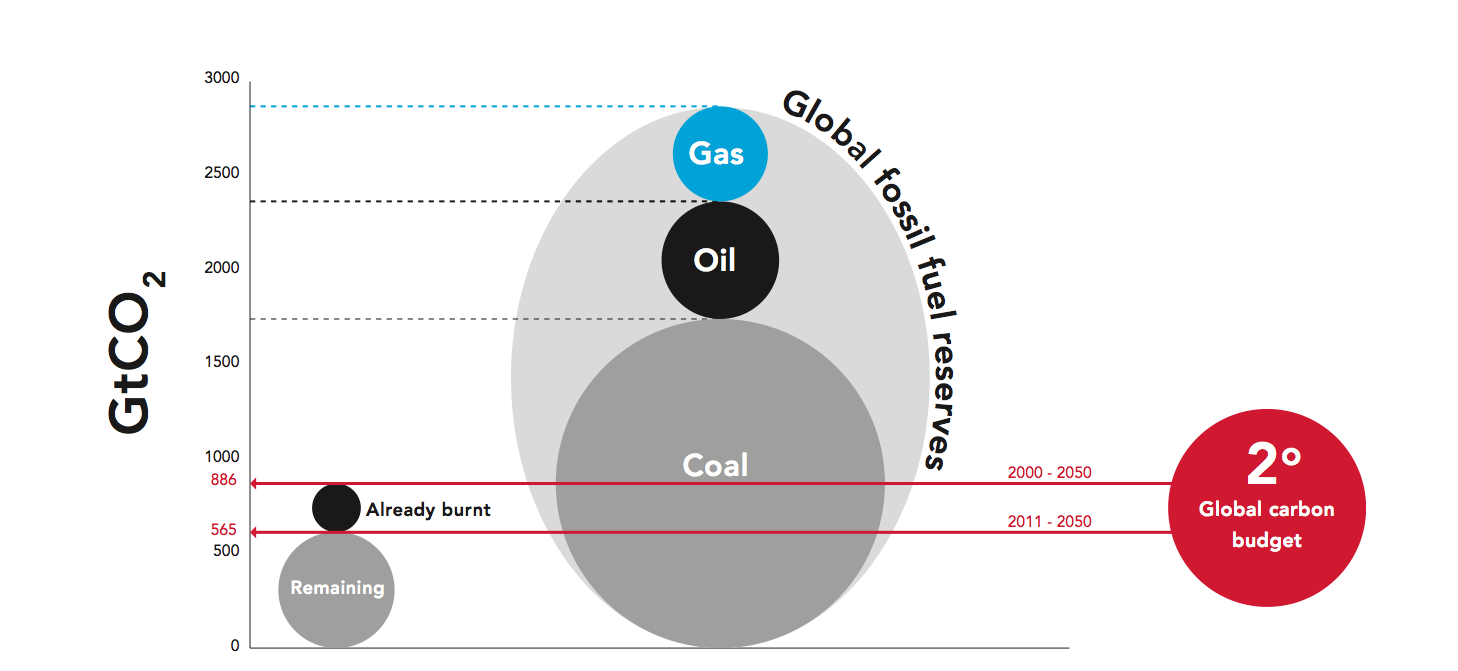
\includegraphics[width=\textwidth]{s1-carbon-budget.png}
\centering
\caption{Comparison of the global 2˚C carbon budget with fossil fuel reserves \ce{CO2} emissions potential. Source: Carbon Tracker Institute, ``Unburnable Carbon: Are the world's financial markets carrying a carbon bubble?'', p. 6}
\label{fig:TwoDegreeBudget}
\end{figure}



Figure \ref{fig:TwoDegreeBudget} from the Carbon Tracker Initiative summarizes the situation in which the world now finds itself, in terms of the size of fossil fuel reserves and the safe operating parameters of the planet.
On the left are two circles depicting the total `carbon budget' the world can make use of without breaching the ``dangerous'' 2˚C barrier.
The black circle shows what has already been burned and the grey circle shows what could still be burned without breaking the budget limit.
The circles to the right depict the massive quantity of potential \ce{CO2} emissions embedded in the world's remaining coal, oil, and gas.\footcite[][p. 6]{CTI2012}
The world won't be able to shift instantly to zero-carbon forms of energy, but if we are to avoid breaching the limit we have chosen, we need to stop building new fossil-fuel infrastructure that will burden the world for decades and delay investment in forms of energy that can be relied upon indefinitely.
We need to stop funding the worldwide search for unconventional fossil fuel reserves like oil sands, shale gas, and oil under what remains of the arctic ice.
These objectives can be achieved without sacrificing strong financial performance, and while upholding the values of the university. 




\textbf{How the University of Toronto can make a difference}



The International Energy Agency expects \$37 trillion to be spent on energy supply infrastructure between 2012 and 2035.\footcite[][]{IEA2012factsheet}
Humanity must decide whether to spend this money digging ourselves deeper into a pit of fossil fuel dependence, or whether to redirect it toward moving beyond fossil fuels.
The University of Toronto can help lead the necessary redirection of investment that will allow humanity to prevent climatic catastrophe while building a safe and efficient global energy system that can be relied upon indefinitely.
One of the most effective means the university can employ is selling its shares in fossil fuel companies.
As with divestment from Apartheid South Africa and the tobacco industry, this choice would make a powerful statement about the kind of future the university wishes to help bring about.
It would also help strip the fossil fuel industry of its social license to operate --- a privilege it is proving unworthy of as it pushes the world heedlessly toward climatic catastrophe while imposing harm on innocent people around the world and in future generations.
By selling its holdings before investors at large accept that most of their reserves are unburnable, the university can mitigate against the risk that fossil fuel stock values will fall substantially as the world realizes that their reserves are too dangerous to burn.



Universities, which collectively have endowments and pension funds worth many billions of dollars, can play an important role in driving this shift toward cost-effective approaches to \ce{CO2} mitigation, including energy conservation and renewable energy deployment.\footcite[The consultancy McKinsey \& Company has studied and ranked global options for mitigating GHG pollution, in terms of their cost, plausible deployment speed, and the scale at which they can help solve the problem. See: ][p. 8]{McKinseyCurve}
University divestment of fossil fuel company shares would demonstrate that the `smart money' is sufficiently concerned about climate change to take meaningful action, and could prompt other investors to reconsider their own investment decisions. 
Divestment would help reduce the danger from climate change by decreasing investor confidence in the viability of new projects like coal-fired power plants and oil pipelines.
As the analysis below demonstrates, it could do so while maintaining an overall portfolio with stable and attractive returns.
The legacy of U of T's investments can either be the continued support for projects that clash fundamentally with what we know to be required to preserve a safe climate, or it can be the development and deployment of energy options that are compatible with enduring prosperity for the university and humanity as a whole.



The authors and supporters of this brief call upon the University of Toronto to:
\begin{itemize}
	\item Make an immediate statement of principle, expressing its intention to divest its direct holdings of stock in fossil fuel companies within five years,
	\item Immediately stop making new investments in the industry,
	\item Instruct its investment managers to wind down the university's existing direct stock holdings in the 200 fossil fuel companies listed in \nameref{sec:200Companies} over five years, and
	\item Divest from Royal Dutch Shell by the end of 2013.
\end{itemize}



Divestment from Royal Dutch Shell should be a high priority for the University of Toronto. 
In addition to being a major contributor to climate change, Shell has an ongoing history of social injury, both in Canada and around the world. 
As the university's single largest international equity holding, Shell sends the message that the University of Toronto is committed to fossil fuel exploitation and unconcerned about the legal and human rights records of the companies in which it invests. 
Divestment would send the opposite message: that the university is committed to addressing climate change, and willing to start emphasizing that commitment by selling its holding in a particularly problematic investment.  
The university would not suffer financially as a consequence of divesting from Shell and, by doing so, it would protect itself from the risks created by this investment.\footnote{See: \nameref{sec:Shell}}



Across North America, the peer schools of the University of Toronto are considering divestment.
These include Harvard, Yale, Princeton, Stanford, and MIT.
[NUMBER] schools have already committed to divest.\footnote{For an up-to-date list, see: \url{http://gofossilfree.org/commitments/}}
By leading the way and becoming the first major university to divest, the University of Toronto can distinguish itself as being ahead of the pack on one of the major issues of the 21st century.



\begin{vcom}
Finalize the number of schools in the paragraph above when the rest of the brief is done.
\end{vcom}



The University of Toronto's Statement of Institutional Purpose includes ``a resolute commitment to the principles of equal opportunity, equity and justice''.\footcite{InstitutionalPurpose}
If future generations are to have equal opportunities, they cannot inherit a planet that has been impoverished by uncontrolled climate change.
Similarly, the principles of equity and justice forbid us from ignoring what we know about the harms of GHG pollution by continuing to impose risk and suffering on innocent people around the world and in future generations.
Canada, Toronto, and the University of Toronto have historically benefitted from fossil fuel use far exceeding the global \emph{per capita} average.
Having benefited for decades from behaviour that we now know to be extremely damaging, the university also has a special moral obligation to be part of the solution.


This brief will explain in detail why a decision to divest would improve the financial prospects of the university, uphold its values, and permit the school to take a leadership role in a necessary global transition away from \ce{CO2}-intensive forms of energy. 



% END SECTION 1 - MILAN

% END SECTION 1 - MILAN



\tableofcontents



% BEGIN SECTION 2 - MILAN
% CLIMATE CHANGE IS SETTLED SCIENCE

% BEGIN SECTION 2 - MILAN
% Last updated by Milan Ilnyckyj 2013-07-30



		\singlespacing
		\section{Climate change is settled science}
		\label{sec:SettledScience}
		\doublespacing



% Has incorporated comments from Alena Prazak and Mie Inouye


	
	\subsection{From the U of T divestment policy}



\begin{itquote}	
The University's core academic values include freedom of inquiry and open debate.
As a general matter, the University does not take positions on social or political issues apart from those directly pertinent to higher education and academic research. 
Instead, its role is to provide a forum within which issues can be studied carefully and debated vigorously. 
Given these values, the University will not consider any proposals for restrictions on its investments that require the institution to take sides in matters that are properly the subject of ongoing academic inquiry and debate.
\end{itquote}



	\subsection{It is not properly the subject of ongoing academic debate that}



\begin{itemize}
	\item The 10,000 years of human civilization have taken place during a span of relative climatic stability.\footnote{This claim is supported by evidence from ice core samples taken in Vostok, Antarctica as well as other proxy measures of climate such as pollen in lake sediments and tree rings.}\footcite[][p. 4]{Alley2000}
	\item Burning coal, oil, and gas produces known quantities of carbon dioxide (\ce{CO2}).\footcite[For example, the U.S. Environmental Protection Agency lists quantities of \ce{CO2} produced by burning a barrel of oil, metric tonne of coal, or therm (100,000 British thermal units) of natural gas:][]{CalculationsReferences}
	\item Before the industrial revolution, the concentration of \ce{CO2} in the atmosphere was approximately 280 parts per million (ppm).\footnote{Evidence for this includes the records of how much fossil fuel has been burned, as well as the changing isotopic ratio of carbon in the atmosphere.}\footcite[][]{IPCC4ARdrivers}
	\item It has now risen to over 390 ppm, largely because of the burning of fossil fuels.\footcite[][]{KeelingExplanation} \footcite[][p. xiv]{WorldBank4C}
	\item Humanity is now adding 31.6 billion tonnes of \ce{CO2} to the atmosphere annually, causing the atmospheric concentration to rise at a rate of approximately 2.0 ppm per year.\footcite[][]{RedrawingClimateEnergy} \footcite[][]{NOAATrends} \footcite[See also: ][]{FaustianGrowth}
	\item If humanity continues to burn fossil fuels at the present rate, the concentration of \ce{CO2} in the atmosphere will rise to well over 550 ppm by 2100.\footcite[][]{IPCCCO2proj}
	\item Adding carbon dioxide to the atmosphere reduces the amount of energy the Earth radiates into space. This causes the planet to warm.\footcite[][]{IPCC4ARdrivers}
	\item Based on evidence from ice cores, we know that doubling the amount of \ce{CO2} in the atmosphere causes global temperatures to rise by about 3˚C.\footcite[][p. 473]{SafeOperatingSpace}
	\item Governments around the world, including the government of Canada, have adopted 2˚C as the threshold beyond which climate change should be considered `dangerous'.\footcite{CopenhagenAccord} \footcite[][p. 5]{CriticalDecade2013} \footcite[See also: ][p. 473]{SafeOperatingSpace} \footcite[See also: ][]{EmGapReport}
	\item If the world is to avoid crossing the 2˚C limit, most of the world's remaining fossil fuels must be kept in the ground.\footcite[][]{IEA2012} \footcite[][]{EconomistUnburnable} \footcite[][]{TerrifyingNewMath} \footcite[The Australian government's Climate Commission states that most fossil fuels must be left in the ground and cannot be burned ][p. 5]{CriticalDecade2013} \footcite[][]{ChallengeTwoDegrees} \footnote{For a detailed rebuttal of the argument that carbon capture and storage eliminates this necessity, see: \nameref{CCSSaves}.}
\end{itemize}


As depicted in figure~\ref{fig:Vostok}, human activity --- especially fossil fuel burning --- has already pushed the level of \ce{CO2} in the atmosphere  far outside the range that has existed for hundreds of thousands of years. Burning the world's remaining fossil fuels would put us even farther outside the climatic conditions experienced by any human civilization to date.
We can also be confident in attributing the warming we have observed to human GHG emissions.
Figure~\ref{fig:CO2increase} illustrates how climate models that incorporate all known natural climate forcings, but which exclude the effect of greenhouse gases, cannot account for observed temperature changes. 
Models that incorporate the greenhouse effect from GHG pollution accord with observations on all continents and the global ocean.\footcite[][]{IPCC2007}



\begin{figure}
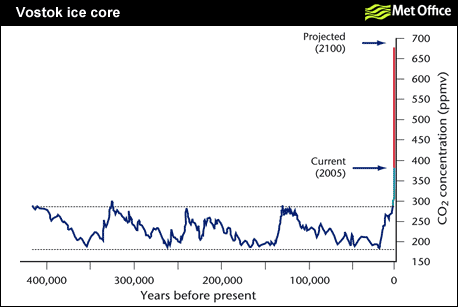
\includegraphics[width=100mm]{s2-co2increase.png}
\centering
\caption{\ce{CO2} concentrations in an ice core from Vostok, Antarctica. Source: U.K Met Office}
\label{fig:Vostok}
\end{figure}



\begin{figure}
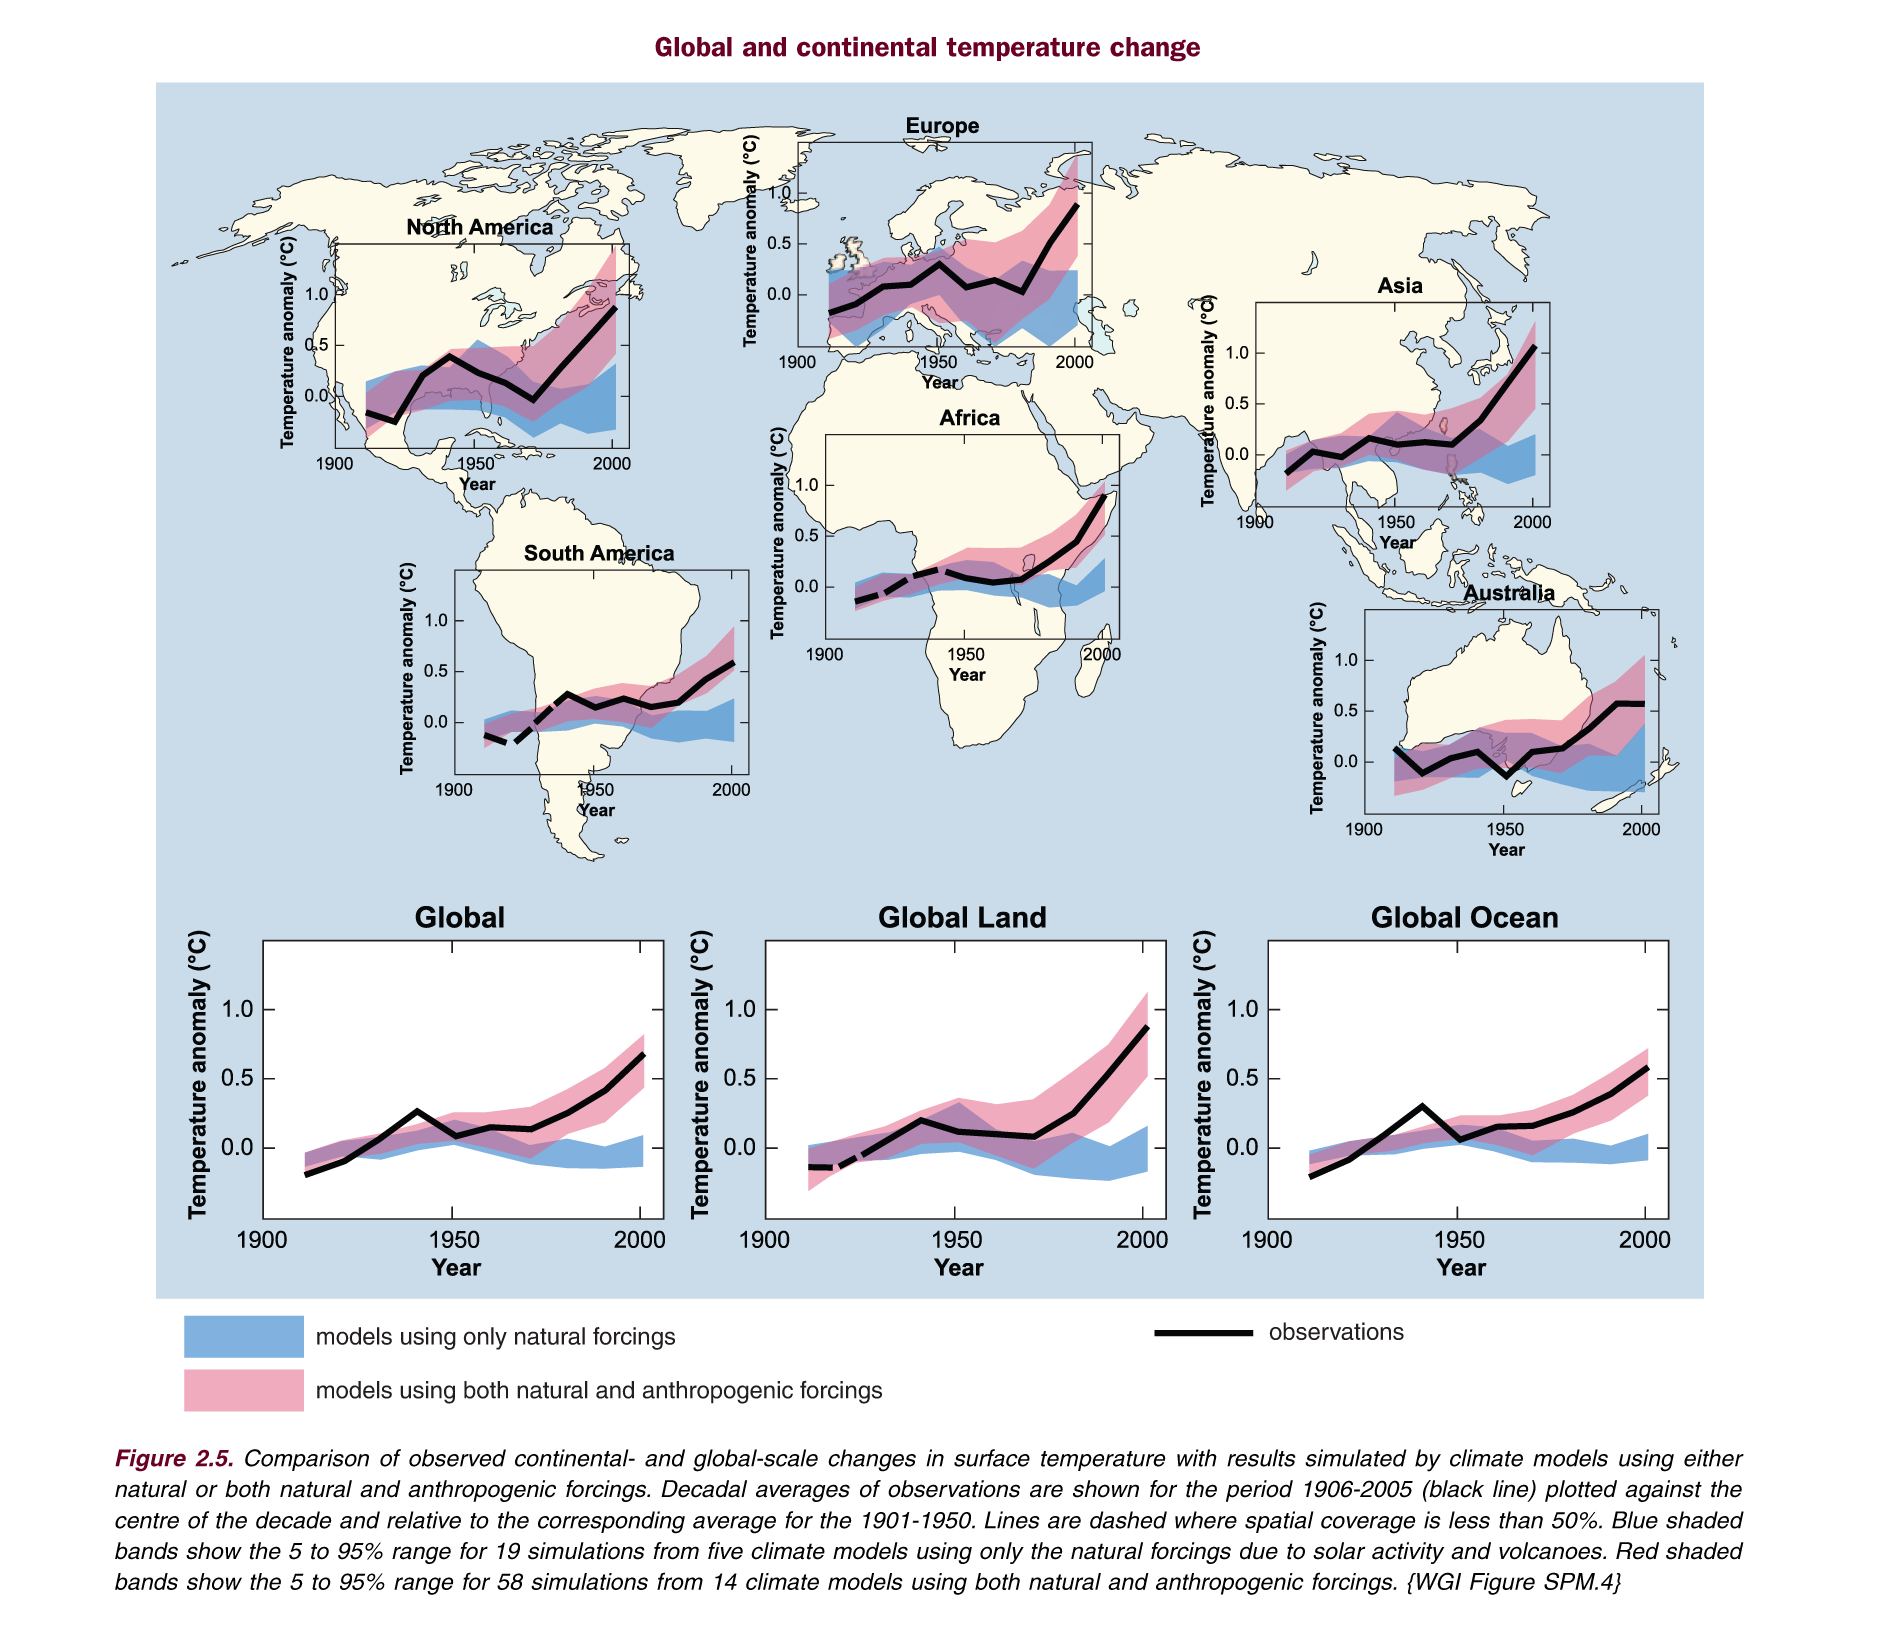
\includegraphics[width=160mm]{s2-attribution.PNG}
\centering
\caption{Global and continental temperature change. Source: IPCC 4th Assessment Report, Synthesis Report, p. 40}
\label{fig:CO2increase}
\end{figure}



Comprehensive and authoritative scientific statements on the key elements of climate change date back at least to the 1979 U.S. National Academy of Sciences report (the Charney report).\footcite[][]{Charney1979}
The report concluded that human activities --- particularly greenhouse gas emissions --- were altering the climate in potentially dangerous ways.
The science of climate change has been extensively examined by the Intergovernmental Panel on Climate Change (IPCC): a body established in 1988 by the World Meteorological Organization and the United Nations Environmental Programme to be the leading international body on the scientific, technical, and socio­economic assessment of climate change.
The four major reports of the IPCC in 1990, 1995, 2001, and 2007 have confirmed the basic conclusions of the Charney report, and elaborated considerably upon the causes and consequences of climate change.\footcite[][]{IPCC1990}\footcite[][]{IPCC1995}\footcite[][]{IPCC2001}\footcite[][]{IPCC2007}
In May 2009, the national science academies of the G8 countries plus Brazil, China, South Africa, and India released a remarkable joint statement.\footcite[][]{G8plusJointStatement}
The statement explains that: ``The need for urgent action to address climate change is now indisputable. For example, limiting global warming to 2°C would require a very rapid worldwide implementation of all currently available low carbon technologies''.
Among other things, it recommends that all governments ``adopt a long-term global goal and near-term emission reduction targets that will deliver an approximately 50\% reduction in global emissions from 1990 levels by 2050'' and ``collaborate in the implementation of low carbon and climate-resilient infrastructure and technologies, and in the implementation of innovative incentives, through the use of economic and regulatory instruments, to accelerate adoption of clean “green” technologies''.
These findings are echoed in recent research, including a 2013 article in \emph{Nature Climate Change} that emphasized how: ``[a] shift to a 2˚C pathway requires immediate significant and sustained global mitigation''.\footcite[][p. 1]{ChallengeTwoDegrees} \footcite[See also: ][]{EmissionTargetsTwoDegrees}



Several significant studies have examined the state of the scientific consensus on climate change.
In 2004, Naomi Oreskes published a paper in \emph{Science} that quantified this.
She examined the abstracts from 928 peer-reviewed papers and found that all of them either take no position on climate change or endorse the consensus position.\footcite[][p. 1686]{Oreskes2004}
She concludes:
\begin{quote}
This analysis shows that scientists publishing in the peer-reviewed literature agree with IPCC, the National Academy of Sciences, and the public statements of their professional societies. Politicians, economists, journalists, and others may have the impression of confusion, disagreement, or discord among climate scientists, but that impression is incorrect.\footcite[][p. 1686]{Oreskes2004}
\end{quote}
Oreskes' book \emph{Merchants of Doubt} elaborates on the article, discussing the strength of this consensus, while also providing details on the active campaigns of disinformation that fossil fuel companies have directed at decision-makers and the general public. \footcite[][]{MerchantsDoubt} \footcite[See also: ][]{ClimateCoverUp}
In 2010, a meta-analysis found that: ``97–98\% of the climate researchers most actively publishing in the field agree with the occurrence of anthropogenic climate change as outlined by the Intergovernmental Panel on Climate Change'' and ``the relative climate expertise and scientific prominence of the researchers unconvinced of climate change are substantially below that of the convinced researchers''.\footcite[][p. 1]{ExpertCredibility}
More recently, a study examined 11,944 climate-related abstracts from 1991 to 2011 and concluded that: ``[a]mong abstracts expressing a position on AGW, 97.1\% endorsed the consensus position that humans are causing global warming''.\footcite[][]{QuantConsensus}


Mitigating climate change is necessary in order for the university to achieve its academic mission. 
In the event that the world fails to curb greenhouse gas emissions and produces well over 2˚C of climate change, substantial damage is expected to be imposed on the global economy.
The Stern Review on the economics of climate change concluded that under a business-as-usual scenario, there is ``at least a 50\% risk of exceeding 5°C global average temperature change'' and that ``[s]uch changes would transform the physical geography of the world. A radical change in the physical geography of the world must have powerful implications for the human geography - where people live, and how they live their lives.''\footcite[][See long executive summary at: \url{http://www.hm-treasury.gov.uk/d/Executive_Summary.pdf}]{Stern2007}
Such an outcome threatens the growth prospects of the endowment and pension funds of the University of Toronto. 
It also creates additional geopolitical risks such as agricultural disruption and forced migration.



% Some of the text in the paragraph below is also in the FAQ section



James Powell, former President of Oberlin, Franklin and Marshall, and Reed College, has concluded that university trustees have a quasi-legal duty to do all they can about climate change, arguing:
\begin{quotation}
The board is supposed to make sure that the endowment allows for intergenerational equity, that the students who are going to Oberlin in 2075 get as much benefit from it as those there now. But with global warming, you’re guaranteeing a diminution of quality of life decades out.\footcite[][]{CaseForDivestment}
\end{quotation}
The emergence of a strong academic consensus about the key features of a problem does not mean that all academic work on the subject ceases.
For instance, scholarly work is still done on South African apartheid, despite the system having been dismantled.
When the university decided to divest from South Africa, it determined that a convincing body of evidence supporting that choice had been assembled.
A comparable body of evidence now exists about the causes and dangers of climate change.
Taking action to address climate change is not an example of needlessly taking sides in a controversial issue. Rather, it is a matter of taking part in a necessary global transition. 
If the world fails to constrain the worst impacts of climate change, serious deleterious impacts can be expected for Canada and the University of Toronto.



	\subsection{The University of Toronto is already taking action on climate change}
	\label{UTTakenSides}



The university has already taken a number of actions motivated by concern about climate change and a desire to reduce the university's greenhouse gas pollution impact.
The university's actions show climate change to be ``directly pertinent to higher education and academic research'', as required by the \nameref{PolicySocialPolitical}.



In November 2009, the University of Toronto signed the ``Ontario Universities Committed to a Greener World'' pledge. In part, the pledge reads:
\begin{quote}
The Ontario university community is deeply aware of the challenges that face the world arising from climate change and the degradation of natural environments. Our universities accept this special responsibility on three scores: to assist in finding solutions to the challenges of environmental sustainability; to share knowledge about sustainability and climate change; and to incorporate, wherever possible, principles of sustainability into our own operations.\footcite[][]{OntarioPledge}
\end{quote}
The decision to divest from fossil fuels stocks would be wholly in keeping with these objectives.
Redirecting investment away from fossil fuels is a key part of solving the challenge of environmental sustainability.
Furthermore, by taking the lead and choosing to divest, the University of Toronto would send an important signal about how it views the future of energy.
This is also an opportunity to incorporate sustainability into university operations in a critical way, by having the university's values reflected in its stock portfolio.



\textbf{Policies and infrastructure decisions justified with reference to climate change}
\label{UofTActions}



% This section incorporates text provided by Jessica Vogt



In 2010, the university adopted an Environmental Protection Policy.\footcite[][]{UTEnvProtectionPolicy}
The policy recognizes that ``that some of [the univeristy's] activities, because of their scale and scope, have the potential, if not managed in compliance with the university’s established standards and practices, to have significant effects on the environment''.
These activities include the investments made by U of T.
Among the principles listed, the policy says the university will:
\begin{itemize}
	\item Operate so as to minimize negative impacts on the environment,
	\item Adopt practices that reflect the conservation and wise use of natural resources, and
	\item Respect biodiversity
\end{itemize}
The policy also lists the conservation of energy and the reduction of waste as objectives.



In 2004, the university established the Sustainability Office at St. George campus and the Environmental Affairs Office at the Mississauga campus.\footcite[][]{UTSustOffice} \footcite[][]{}
The Environmental Affairs Office tracks the electricity and natural gas use of buildings in real-time, and makes the data available through their building dashboard.\footnote{See: \url{http://buildingdashboard.net/utorontom/}}
In 2007, a Sustainability Office was established at the Scarborough campus.\footcite[See: ][]{UTSustOffice}
This office explains that: ``[a] number of retrofit projects have been undertaken to reduce energy consumption as well as CO2 emissions''.\footcite[][]{UTSustOfficeEnergy}
The Facilities and Services Department provides a breakdown of the university's GHG emissions.\footnote{See: \url{http://sustain.fs.utoronto.ca/campus-footprint/}}
U of T also has a Sustainability Board, charged with providing guidance, support, and coordination of initiatives between the three campuses.



The annual reports of the Sustainability Office include data on the GHG emissions from the St. George Campus.\footcite[][]{UTSustOffice2010report}
The 2010 report partly justifies the installation of a solar hot water system at the Faculty of Physical Education and Health on the basis of reduced GHG pollution.\footcite[][p. 17]{UTSustOffice2010report}
A 2010 press release describes how paper use at the St. George campus produces ``greenhouse gas emissions of about 1,500 tonnes'' and describes how an expanded paper conservation program aims to reduce that.\footcite[][]{UTGoingGreener2010}
In a comparison of sustainability indicators, the 2011 strategic plan of the Sustainability Office lists ``[g]reenhouse gas emissions'' as an area where U of T ``leads''.\footcite[][p. 1]{UTSustOfficePlan}
In particular, it says that the office will ``[w]ork with specific university constituencies... to identify financially sound opportunities for emission reduction''.
The plan also lists ``[c]limate and [r]esources'' under ``priority long-term goals and key actions'' and identifies GHG emissions as a ``key performance indicator''.




\textbf{Academic programming}
\label{UofTAcademicProgramming}


In 2005, the university established a new Centre for Global Change Science (CGCS), which has since conducted exemplary research into climate change effects, as well as a wide array of public lectures focused around climate-related themes.\footnote{See: \url{http://www.cgcs.utoronto.ca/}}
Danny Harvey --- a Professor in the Department of Geography who is associated with the centre, is also the author of two important books describing the causes and consequences of climate change.\footcite[][]{Harvey1999a} \footcite[][]{Harvey1999b}
The CGCS has hosted a number of talks as part of its Distinguished Lecture Series including:
\begin{itemize}
	\item Successes and Challenges for Biodiversity Science: Distribution Responses to Climate Change --- James Clark, Duke University, September 18, 2012
	\item High Altitude Climate Change: The Survival Struggle of our Earth’s Alpine Glaciers --- Andrew Bush, University of Alberta, October 16, 2012 
	\item Assessing Vegetation Responses and Feedbacks to Climate Change --- John Gamon, University of Alberta, November 6, 2012
	\item Cumulative Carbon Emissions and the Climate Mitigation Challenge --- Damon Matthews, McGill University, February 5, 2013; and
	\item Trees to Tailpipes: Natural and Anthropogenic Influences on Global Atmospheric Composition --- Colette Heald Massachusetts Inst. of Technology, March 5, 2013.\footcite[][]{DistinguishedLecturer}
\end{itemize}


The Koffler Scientific Reserve at Jokers Hill is conducting research on how climate change is affecting plant species.\footcite[][]{KofflerCC}
The project is ``using artificial warming field arrays to elevate temperatures to those predicted for 2050''.



The Department of Computer Science operates a weekly seminar series: Collaborative Challenges for the Climate Change Research Community.\footnote{See: \url{http://www.cs.toronto.edu/climate/}}
Recent presentation topics have included climate models, building community resilience to climate change, the response of freshwater ecosystems in Canada's north to climate change, and low-carbon cities.



The university also offers courses on climate-change-related themes, including:
\begin{itemize}
	\item Applied Climate Change: Gaining Practical Skills for Climate Change Adaptation (UTSC Summer Institute 2013)
	\item Gaining Practical Skills for Climate Change Adaptation (UTSC Summer Institute 2013)
	\item Climate Change Law (LAW269H1S); and
	\item Climate Change and Human Health (CEM 406).
\end{itemize}
The University of Toronto also maintains an Environmental Research Database which includes ``430 University of Toronto researchers across all three U of T campuses engaged in environment-related research encompassing a wide spectrum of interests ranging from environmental finance to climate change''.\footcite[][]{UTEnvResDB}



% Material from Stuart incorporated



U of T identifies some of its own faculty as climate change experts.
As part of the university's `Boundless' campaign, Richard Peltier at the Centre for Global Change Science is identified as a ``Physicist and Climate Scientist''.\footcite[][]{PeltierBoundless}
Ron Dembo --- the founder and CEO of Zerofootprint, a software company focused on reducing humanity's environmental footprint --- is also included as one of the campaign volunteers.\footcite[][]{DemboBoundless}
On his Boundless campaign page, Professor of Public Health Sciences and of Surgery Abdallah Daar identifies climate change as a threat that ``do[es] not carry passports or recognize borders''.\footcite[][]{DaarBoundless}
The Institute of Global Health Equity and Innovation within the Faculty of Medicine lists climate change as an area of research.\footcite[][]{GlobalHealthEquity}
Along with Lorraine Sugar from the World Bank, Professor Chris Kennedy, at the Department of Civil Engineering, co-authored ``A low carbon infrastructure plan for Toronto, Canada'' in the \emph{Canadian Journal of Civil Engineering}.\footcite[][p. 86-96]{Sugar2012}
They estimate that implementation of their strategies could produce a 31\% reduction in per capita GHG emissions by 2031.



Climate change is certainly an area of active scholarly research, but that research does not question the fundamental connection between burning fossil fuels and warming the planet. 
Nor does it challenge the argument that climate change is likely to cause a great deal of social injury and human suffering.
Rather, the academic work being conducted on climate change at U of T reinforces the case for divestment.



	\subsection{Fossil fuel companies acknowledge the reality and danger of climate change}



% Ideally, this section should be read while listening to Leonard Cohen's "Everybody knows"

	

Fossil fuel companies explicitly acknowledge that climate change poses a threat to the world at large, as well as to their operations and profitability.\footcite[][]{FFcorpsPlanning} \footcite[][]{OilCosFearFI} \footcite[][]{DemiseOfCrudeDenial} \footcite[][]{DoTheOpposite}
In their 2011 submission to the Carbon Disclosure Project, ExxonMobil acknowledged ``risks to society and ecosystems from rising greenhouse gas emissions''.\footcite[][]{ExxonCDP2011}
In the same document, ExxonMobil acknowledges that climate change may alter ``risks of weather extremes'' and states that they ``manage these risks through robust design and operations contingency planning''.
Speaking at the Council on Foreign Relations on June 27th 2012, ExxonMobil CEO Rex Tillerson stated: `` So I'm not disputing that increasing \ce{CO2} emissions in the atmosphere is going to have an impact. It'll have a warming impact.''\footcite[][]{Tillerson}
On their website, ConocoPhillips recognizes that: ``human activity, including the burning of fossil fuels, is contributing to increased concentrations of greenhouse gases (GHG) in the atmosphere that can lead to adverse changes in global climate''.\footcite[][]{ConocoPhillipsCC}
They also assert that ``effective climate change policy must... [r]esult in the stabilization of global GHG atmospheric concentrations at safe levels''.
On their global website, Shell says that: ``\ce{CO2} emissions must be reduced to avoid serious climate change''.\footcite[][]{ShellClimateChange} \footnote{Shell also has a climate change advisor, with a blog at: \url{http://blogs.shell.com/climatechange/}}
Chevron's website asserts that: ``a successful climate policy will be one in which the reduction of GHGs is accomplished equitably by the top emitting countries of the world through long-term and coordinated national frameworks''.\footcite[][]{}
On BP's website, they summarize the conclusions of the Intergovernmental Panel on Climate Change and say that even with more aggressive GHG mitigation policies growth in \ce{CO2} emissions will ``probably not [be] enough to limit warming to no more than 2˚C''.\footcite[][]{BPClimateChange}
Entergy --- an S\&P 500 company with nearly 15,000 employees --- also acknowledges material risks from climate change.
Jeff Williams, director of climate consulting for Entergy, states: ``Clearly we are facing risks from sea level rise, more intense storms, flooding and surge damage''.\footcite[][]{ShiftToClimatePreparedness}


In numerous advertising campaigns, fossil fuel companies have acknowledged that climate change is taking place, and even that they bear some responsibility for dealing with it.
At the same time, much of the fossil fuel industry's advertising is misleading in its description of environmental effects.
For instance, recent advertising in Canada has misrepresented the effect of oil sands extraction on freshwater.\footcite[][]{PembinaOilAds}


\begin{vcom}
There are lots of greenwashing ads - possibly even from Shell - that we can use to demonstrate that the fossil fuel industry itself acknowledges climate change.
\end{vcom}



As elaborated in \nameref{sec:LikeTobacco} there are many parallels between fossil fuel divestment and divestment from tobacco companies.
Among these the awareness of the producers themselves that their products are harmful and dangerous.
When the University of Toronto decided to divest from tobacco companies, President David Naylor noted the significance of tobacco companies themselves acknowledging the health risks of smoking: ``that there is no serious academic or social debate about tobacco's health effects – even tobacco manufacturers by now concede them.''\footcite[][]{TStarSellOff}



% END SECTION 2 - MILAN

% END SECTION 2 - MILAN



% BEGIN SECTION 3 - TAMARA AND MIE
% SOCIAL INJURY

% BEGIN SECTION 3 - MIE
% Last updated by Milan Ilnyckyj 2013-08-12



		\singlespacing
		\section{The activities of fossil fuel companies are socially injurious, and this social injury cannot be reasonably remedied through shareholder voice}
		\label{sec:SocialInjury}
		\doublespacing



% Has incorporated comments from Alena Prazak



	\subsection{From the U of T divestment policy}



\begin{itquote}
Social injury is the injurious impact which the activities of a company are found to have on consumers, employees, or other persons, particularly including activities which violate, or frustrate the enforcement of, rules of domestic or international law intended to protect individuals against deprivation or [sic] health, safety, or basic freedoms; for purposes of this Policy, social injury shall not consist of doing business with other companies which are themselves engaged in socially injurious activities.
\end{itquote}



	\subsection{Social injury}


The primary activities of fossil fuel companies impose social injury on consumers, employees, or other persons.
The burning of a large portion of the world's reserves of fossil fuels would inflict great social injury through:
\begin{enumerate}
\item Impacts on agriculture
\item The inundation of coastal areas
\item Storms, droughts, other extreme weather
\item Wildfires
\item Increased risks to human health
\item Ecosystem collapse 
\item Threats to First Nations groups and indigenous cultures
\item Threats to the infrastructure of cities, including Toronto
\item The threat of abrupt and non-linear adverse climate impacts, arising from positive feedback effects and important thresholds in the climate system
\item Security implications
\end{enumerate}
In their 2007 report, the IPCC included a table (shown in figure~\ref{fig:IPCCImpacts}) that summarized how various forms of injury associated with climate change can be expected to worsen as the amount of warming increases.



\begin{figure}
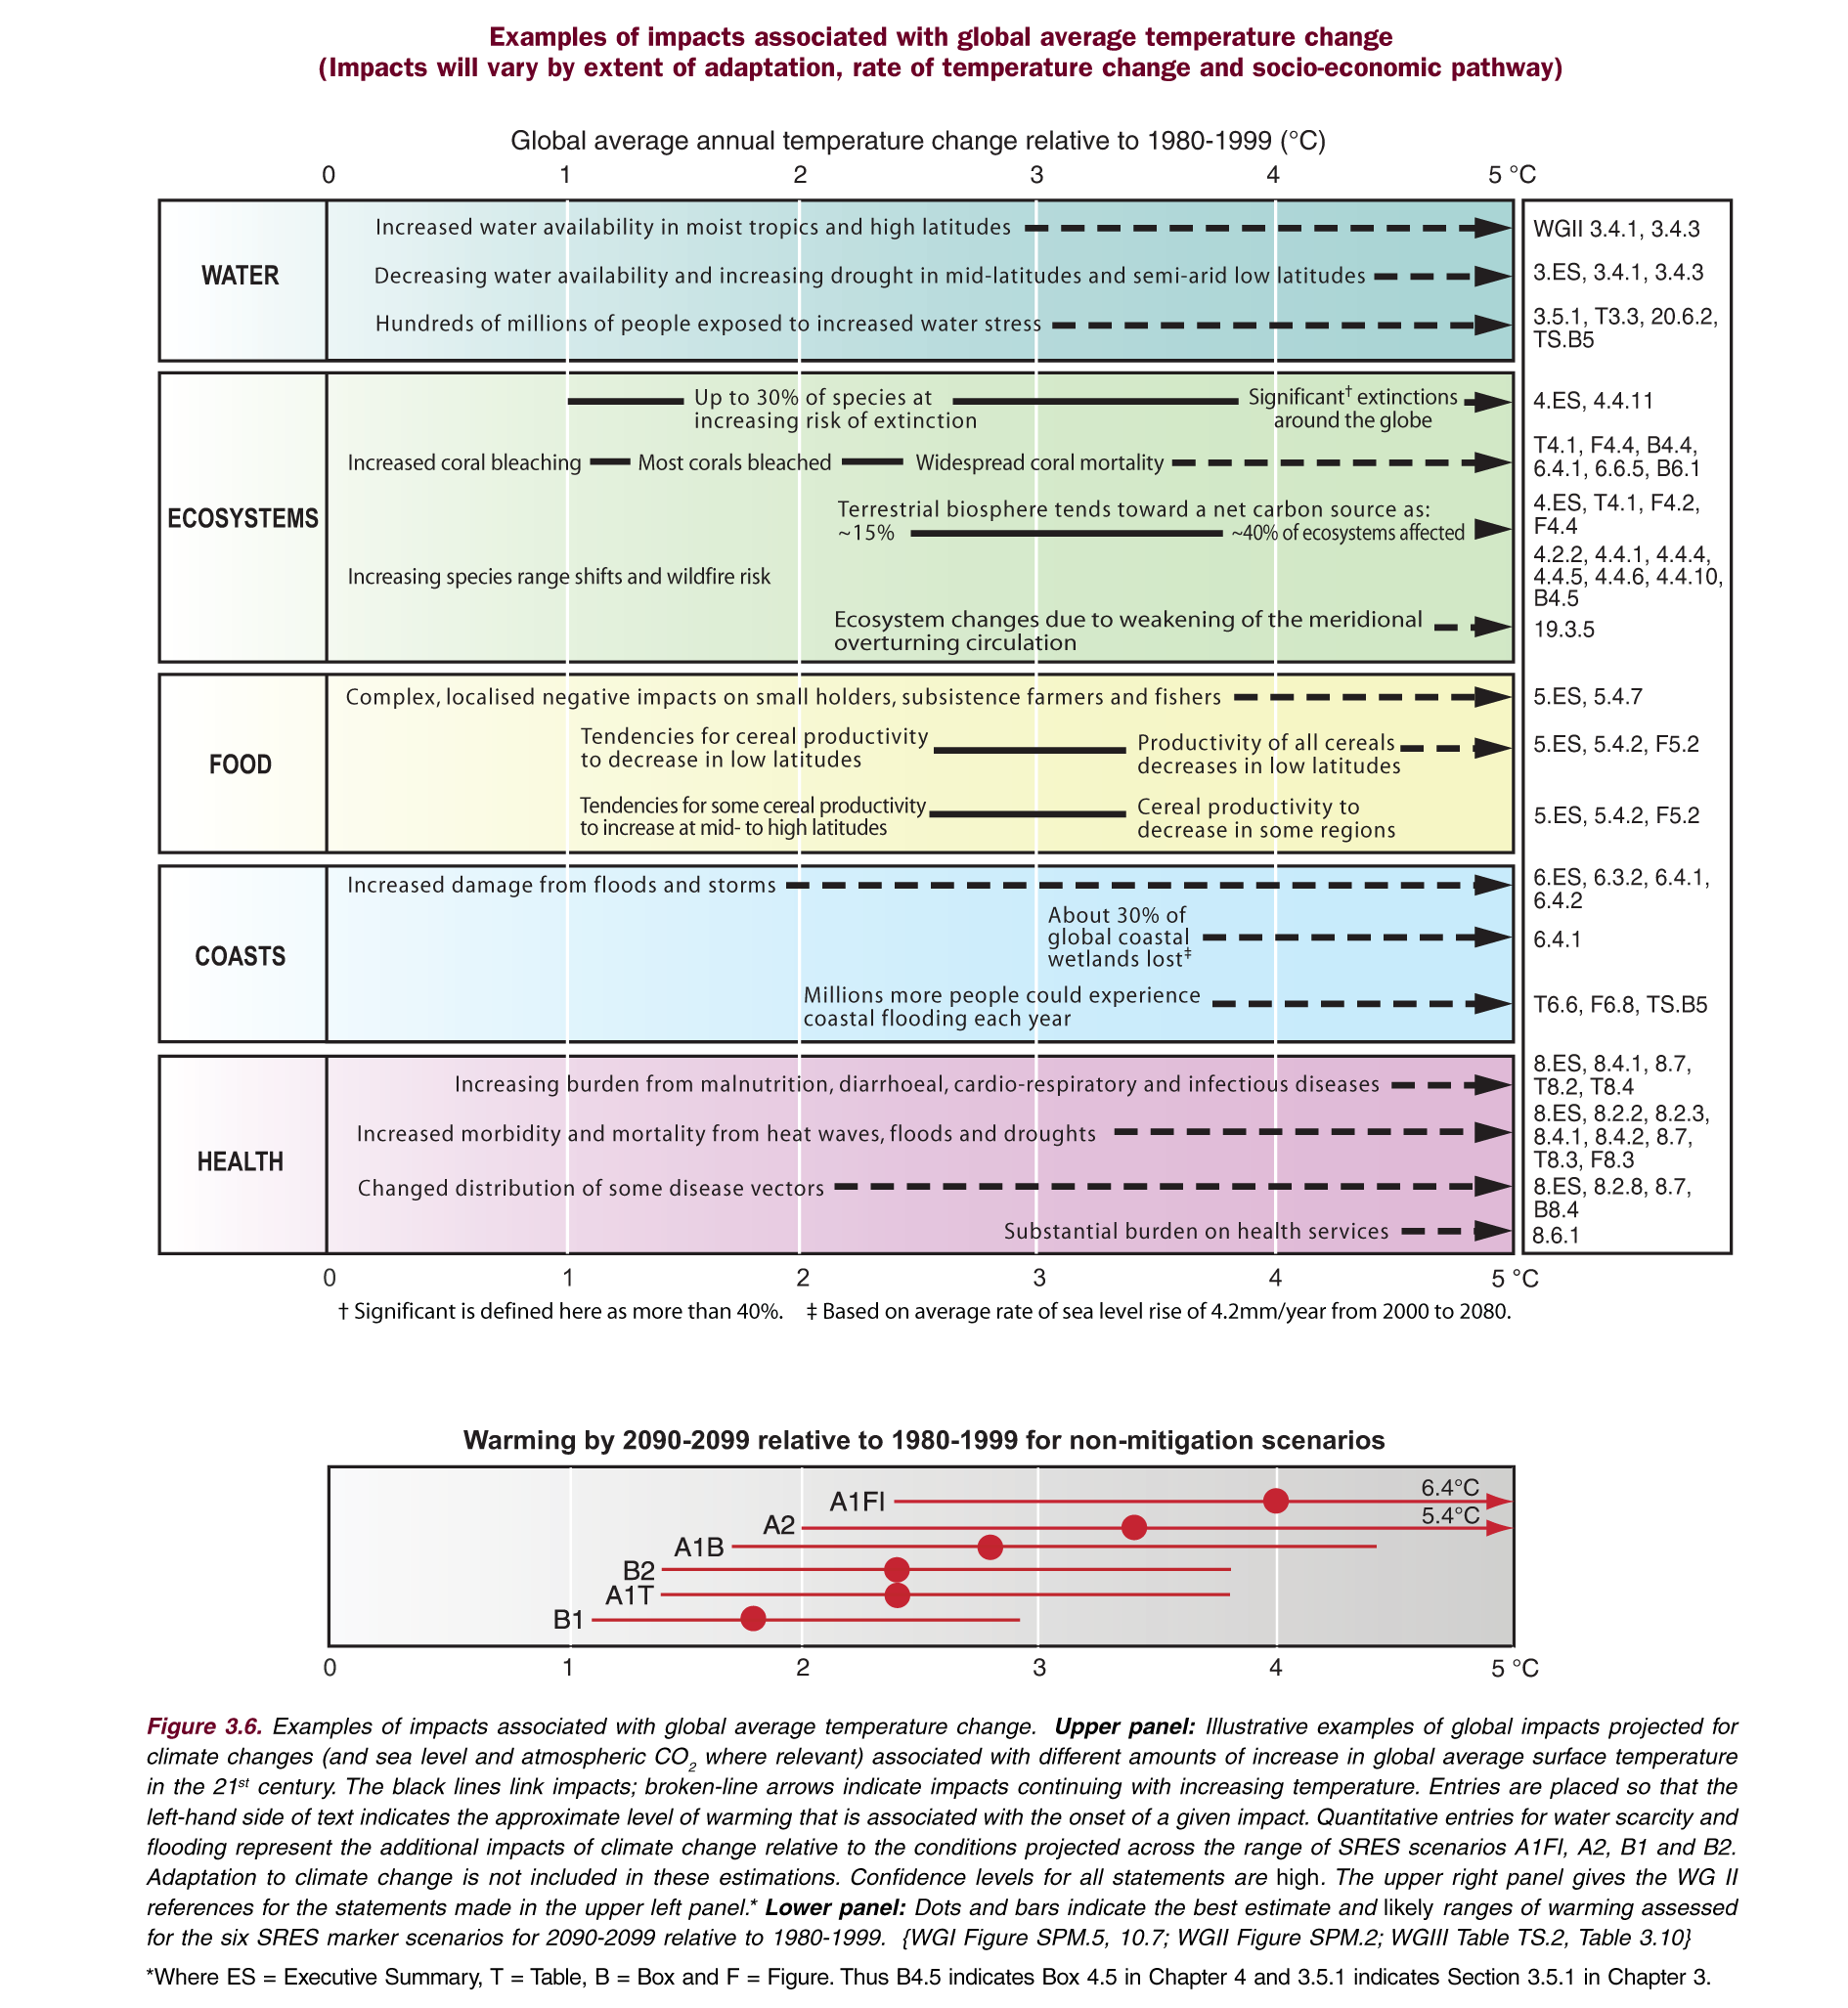
\includegraphics[width=160mm]{s3-variousimpacts.png}
\centering
\caption{Examples of impacts associated with global average temperature change. Source: IPCC 4th Assessment Report, Synthesis Report, p. 51}
\label{fig:IPCCImpacts}
\end{figure}



Each of these impacts has consequences for human beings, and each represents a form of social injury being imposed on innocent people by the producers of fossil fuels.
According to the United Nations Development Programme, ``climate change... already imposes substantial costs, with the brunt of them borne by poor countries and poor communities''.\footcite[][p. 34]{UNHumanDev2013} \footcite[See also: ][]{WorldBankDevCC}
This harm is not exclusively imposed on poor countries, and can be expected to worse in a business-as-usual scenario: ``Climate change and local stresses on natural resources and ecosystems are increasing pressure on the environment in almost all countries, regardless of their stage of development. Unless action is taken urgently, future progress in human development will be threatened.''\footcite[][p. 87]{UNHumanDev2013}
A 2009 report by the Global Humanitarian Forum concluded that: ``every year climate change leaves over 300,000 people 
dead, 325 million people seriously affected, and economic losses of US\$125 billion''.\footcite[][p. 1]{AnatomySilentCrisis}



According to the 2009 report ``Adapting to Climate Change in Ontario: Towards the Design and Implementation of a Strategy and Action Plan'' produced by the Expert Panel on Climate Change Adaptation, Ontario is expected to experience a temperature increase of 2.5°C to 3.7°C by 2050, compared to mean levels from 1961-1990.\footcite[][p. 15]{ExpertPanelAdapting2009}
These projections are based on moderate assumptions about greenhouse gas reductions; however, estimates based on high emissions scenarios may be more realistic, and predict the a rise of temperature as high as 4.0°C by 2050.



Canada is causing a disproportionate share of damage to the climate, both relative to its population and relative to its share of the global economy.
Furthermore, because of the enormous quantity of carbon embedded in the oil sands, Canada has the potential to single-handedly cause substantial damage to the global climate.\footcite[][]{IrrevocablyTar}



In 2011, the National Roundtable on the Environment and the Economy (NRTEE) concluded that: ``[c]limate change will be expensive for Canada and Canadians. Increasing greenhouse gas emissions worldwide will exert a growing economic impact on our own country, exacting a rising price from Canadians as climate change impacts occur here at home''.\footcite[][p.15]{NRTEEPrice}
They also concluded that: ``Global mitigation leading to a low climate change future reduces costs to Canada in the long term.''\footcite[][p.16]{NRTEEPrice}
The NRTEE highlighted how Canada and the rest of the world must choose between two futures: one in which action is taken (necessarily diminishing the profits and stockmarket value of fossil fuel companies) and another in which the world suffers the unmitigated consequences of climate change:
\begin{quote}
Examining long-term economic costs of climate change to Canada raises the spectre of two futures: one where the world acts — and keeps global warming to 2°C by 2050 as world leaders have pledged — and one where it doesn't and climate change impacts grow and accelerate beyond targets. At slightly under 2°C of global warming, the economic costs of climate change to Canada in 2050 would be between \$21 billion and \$43 billion with no adaptive action taken; costs could be at the lower end of range if economic growth slowed as part of domestic mitigation or for other reasons. If the world acts to limit warming to 2°C, future costs could stabilize around this 2050 level since emissions growth would have been dampened and plateaued to reach this new global reality.\footcite[][p.18]{NRTEEPrice}
\end{quote}
A 2012 NRTEE report identifies ice, snow and sea; ecosystems; water resources; human health; communities and infrastructure; resource industries; service industries; and security and trade as categories in which climate change is expected to have adverse impacts.\footcite[][p. 41]{DegreesOfChange}



In a briefing note prepared for Minister of the Environment Peter Kent and subsequently released through an access to information request, officials at Environment Canada argued that: ``Climate change is the most serious environmental issue facing the world today and carries with it significant impacts on human health and safety, the economy, natural resources, and ecosystems in Canada and throughout the world''.\footcite[][]{BureaucratsUrged}



The \nameref{PolicySocialPolitical} specifies that the University of Toronto will use the Yale University concept of social injury when responding to any petition regarding divestment.\footcite[See also: ][]{EthicalInvestor}
Specifically, the policy defines social injury as:
\begin{itquote}
Social injury is the injurious impact which the activities of a company are found to have on consumers, employees, or other persons, particularly including activities which violate, or frustrate the enforcement of, rules of domestic or international law intended to protect individuals against deprivation or health, safety, or basic freedoms; for purposes of this Policy, social injury shall not consist of doing business with other companies which are themselves engaged in socially injurious activities.
\end{itquote}
Climate change falls within this definition.
The section below lists many injurious impacts fossil fuel companies are having on consumers, employees, and other persons.
It also describes ways in which the behaviour of these companies has frustrated domestic and international law.
The sections below will elaborate on these forms of social injury, providing empirical evidence of the observed adverse impacts and predicted future risks from climate change.



	\subsubsection{Pricing the social cost of carbon}
	\label{sec:PricingSocialCost}



Many organizations have attempted to quantify the ``social cost of carbon'' --- the amount of damage done to third parties by emitting one tonne of \ce{CO2}.
For instance, the U.S. Department of Energy recently increased its estimate from \$22 per tonne to \$36.\footcite[][]{DOE22to36} \footcite[][]{WHStrengthened} \footcite[See also: ][]{NewSocialCostEffort} \footcite[][]{CBCUSSocialCost}
In the United Kingdom, the government has been using a ``shadow cost'' of carbon to estimate social harm since 2007.\footcite[][]{DEFRAShadowCost}
The Department for Environment, Food and Rural Affairs explains that: ``The social cost of carbon (SCC) measures the full global cost today of an incremental unit of carbon (or equivalent amount of other greenhouse gases) emitted now, summing the full global cost of the damage it imposes over the whole of its time in the atmosphere. It measures the scale of the externality which needs to be incorporated into decisions on policy and investment options in government.''
The Stern Review estimated a social cost of carbon of about \$30 per ton of \ce{CO2} equivalent in 2000.\footcite[][]{Stern2007}
In a 2013 study, the World Bank concluded that ``[regional, national and sub-national carbon pricing initiatives are proliferating'', with systems implemented in California, Quebec, Switzerland, the European Union, Kazakhstan, Tokyo, Australia, and New Zealand.\footcite[][p. 11]{WorldBankCarbonPricing}
Systems are also under consideration in Chile, Brazil, Turkey, Ukraine, China, and Japan.
The report explains that ``[n]ew approaches are emerging to ensure ambition and price stabilization'', that ``[n]ational and regional trading schemes are starting to link up'' and that ``[c]limate change requires urgent action at scale''.\footcite[][p. 12--13]{WorldBankCarbonPricing}



In Canada, the National Round Table on the Environment and the Economy has repeatedly argued in favour of putting a price on GHG pollution in order to reflect the harm it does to society.\footcite[See: ][]{Achieving2050} \footcite[][]{Achieving2050Outreach} \footcite[][p. 18]{FramingFuture}
In a 2012 report, they highlighted the costs of delaying the implementation of a price on carbon:
\begin{quote}
The NRT analysis for Environment Canada reinforces a central conclusion of all our work and many other independent sources: delay is costly. Put directly, time is money. The closer the target date approaches, the higher the carbon prices will have to be to incent investment in capital stock turnover, develop and deploy and new technologies, and change firm and household energy-use behaviour.\footcite[][p. 114]{RealityCheck2012}
\end{quote}
``Finding the right price signal'', they conclude, ``is key''.\footcite[][p. 117]{RealityCheck2012}



As pointed out by Peter Foster, determining the appropriate social price of \ce{CO2} is made more complicated by the need to somehow incorporate the worst-case scenarios associated with global climate change.\footcite[][]{ApocExternal}
For instance, if we add enough \ce{CO2} to the atmosphere to cause the eventual disintegration of a large fraction of the world's ice sheets, raising global sea levels by tens of metres, millions of people would be displaced and a huge part of the planet's cultural legacy would be forever destroyed.
It is challenging to identify how such possibilities factor into a per-tonne estimate of the damage caused by GHG pollution.



	\subsubsection{Impacts on agriculture}



Agriculture is widely considered to be one of the most vulnerable systems to climate change in large part because its productivity is highly dependent on stable climate cycles and weather patterns.
For instance, in their Fourth Assessment Report, the IPCC concluded that some African countries agricultural production, including access to food, ``is projected to be severely compromised''.\footcite[][See: Synthesis report, Table SPM.2. Examples of some projected regional impacts. \url{https://www.ipcc.ch/publications_and_data/ar4/syr/en/spms3.html}]{IPCC2007}
Production from agriculture and forestry is expected to decline in Australia and New Zealand by 2030, and in Latin America ``[c]hanges in precipitation patterns and the disappearance of glaciers are projected to significantly affect water availability for human consumption, agriculture and energy generation.''
The 2013 U.N. Human Development Report explained: ``Although low HDI countries contribute the least to global climate change, they are likely to endure the greatest loss in annual rainfall and the sharpest increase in its variability, with dire implications for agricultural production and livelihoods.''\footcite[][p. 6]{UNHumanDev2013}
A report from the International Food Policy Research Institute (IFPRI) found that: ``agriculture and human well-being will 
be negatively affected by climate change''.\footcite[][p. vii]{IFPRIAgri}
The report predicts crop declines in developing countries, especially in South Asia; price increases for the most important agricultural crops, including rice, wheat, maize, and soybeans; lower calorie availability throughout the developing world in 2050 when compared with both a no-climate-change scenario and 2000 levels; 20\% more child malnutrition than in a world with no climate change; and costs of U.S. \$7.1 to \$7.3 billion to raise calorie consumption sufficiently to offset the health impacts of climate change on children.\footcite[][p. vii]{IFPRIAgri}



Changes in climate that will affect Canadian agricultural production include events such as heat waves and droughts, infestation of pests, and severe storms.
The Ontario Ministry of Agriculture and Food's website lists projected impacts including:
\begin{itemize}
	\item increased heat stress on livestock
	\item increased pest volumes and number of pest species
	\item modified geographical extent of agricultural production and locational shifts for growth of certain crops
	\item potential limitations on food processing expansions due to water quality and quantity issues
	\item financial challenges for rural municipalities exposed to extreme weather events and needing large infrastructure enhancements to cope with such events (bridges, roads, etc.)\footcite{OntarioCCandAg}
\end{itemize}
Climate change is also expected to do between \$2 billion and \$7 billion in damage to Canada's timber industry by 2050, ``through changes in pests, fires, and forest growth''.\footcite[][p.16]{NRTEEPrice}



Studies exploring economic approaches to dealing with climate change show that adaptation can provide one route to alleviate risks to Canada's agricultural sector.\footcite{Amiraslany2010}
However, extreme weather events, which are predicted to occur with increasing frequency as global temperatures rise are significant drivers of yield and impact changes and can therefore disrupt adaptation practices and threaten the health and prosperity of agricultural systems.\footcite{IsikDevadoss2006}
Indeed, possibilities of extreme weather events are often outside the scope of adaptation policies that outline strategies and recommendations for coping with less acute impacts such as those listed above.\footcite[See for instance:][]{Malcolm2012}



The ongoing drought in the United States provides a glimpse of what may become increasingly routine in a world altered by climate change.
Beginning in the spring of 2012, the drought originally affected areas along the plains and western mid-west regions of the country. 
As the drought continued, the federal government declared most of the central and southern U.S. wheat belt a natural disaster area. 
By July, the drought had reached such extreme conditions that officials in north-central Oklahoma declared a state of emergency on account of record-low reservoir conditions. 
Furthermore, the U.S Department of Agriculture (USDA) granted eligibility for low-interest emergency loans to wheat growers in four major wheat-growing states: Kansas, Colorado, Oklahoma and Texas. 
In early 2013, experts from the National Oceanic and Atmospheric Administration's Climate Prediction Center and the National Drought Mitigation Center at the University of Nebraska-Lincoln predicted that, despite various localized improvements, the drought is set to worsen in general through spring 2013, and will in fact expand to affect areas in California, Texas and Florida.\footcite[][]{NOAAteleconf2013}
Martin Hoerling, a research meteorologist at the National Oceanic and Atmospheric Administration, explains that: ``[c]limate change is likely prolonging the duration and severity of naturally occurring drought in the Southwest'' and that both reduced rainfall and higher temperatures may contribute to future droughts.\footcite[][]{USHeatAndDrought}
Moreover, less than average snow accumulation in surrounding areas including the central and southern Rockies, results in a decrease of water flowing from streams and rivers to reservoirs, which adds to concerns about the potential for the drought to increase in scope.



Prolonged heat waves and periods of drought are projected to intensify globally concurrent with accelerating warming of global temperatures caused by the increase of GHG levels in the atmosphere.
The IPCC expects increased incidence of drought in asia, Australia and New Zealand, and Europe.
In North America, it expects ``[w]arming in western mountains... to cause decreased snowpack, more winter flooding and reduced summer flows, exacerbating competition for over-allocated water resources''.\footcite[][See: Synthesis report, Table SPM.2. Examples of some projected regional impacts. \url{https://www.ipcc.ch/publications_and_data/ar4/syr/en/spms3.html}]{IPCC2007}
Canada has experienced significant extreme heat and drought events in its recent history. 
For instance, six wide ranging and severe droughts took place over southern Ontario between 1936 and 1998. 
Two droughts, one in 1988 and the other ten years later in 1998, were both consistent with predictions in climate change scenarios for the Great Lakes region.\footcite[][]{Koshida2005}
In their latest assessment report, the IPCC concluded that ``[c]limate change is expected to exacerbate current stresses on water resources from population growth and economic and land-use change, including urbanisation'' and that areas ``where more than one-sixth of the world population currently lives'' are expected to experience ``[r]educ[ed] water availability, hydropower potential, and changing seasonality of flows in regions supplied by meltwater from major mountain ranges''.\footcite[][p. 49]{IPCCar4_syr}
They also concluded that: ``[t]he negative impacts of climate change on freshwater systems outweigh its benefits (high confidence).''\footcite[][p. 49]{IPCCar4_syr}



In a report prepared for the U.S. Federal Emergency Management Agency, AECOM estimated that the portion of the U.S. at risk from flooding will increase by 45\% by 2100, with 70\% of that increase attributable to climate change.\footcite[][p. ES-7]{FEMAFlood} \footcite[See also: ][]{MJFlood}
As reported by the U.S. Environmental Protection Agency: ``[m]ore extreme temperature and precipitation can prevent crops from growing. Extreme events, especially floods and droughts, can harm crops and reduce yields''.\footcite[][]{EPAAgFoodImpacts}



The IFPRI finds that declines in yields of one critical world crop --- wheat --- will become greater the longer mitigation is delayed. 
Using a 2000 baseline, they project a decline in yield for rainfed wheat in the developed world of 1.3 percent by 2030, 4.2 percent by 2050, and 14.3 percent by 2080.\footcite[][p. 85]{Farming2050}
Up to 2050, climate change's impact on agriculture might be manageable to some extent; however, the IFPRI report concludes: ``Starting the process of slowing emissions growth today is critical to avoiding a calamitous post-2050 future''.\footcite[][p. xxi]{Farming2050}
While adaptation strategies may provide certain methods for dealing with select risks to agricultural production that are directly associated with climate change, mitigation in the form of reducing GHG emissions is essential to the long-term health and prosperity of the agricultural sector in Canada.



	\subsubsection{The inundation of coastal areas}
	\label{sec:inundationcoastal}

	
	
Across Canada, coastal communities, forests, agriculture, and fisheries are increasingly at risk from climate change.\
In the Natural Resources Canada report \emph{Climate Change Impacts and Adaptation: A Canadian Perspective}, ``sea level rise, resulting from thermal expansion of ocean waters and increased melting of glaciers and ice caps'' is identified as ``the main issue for marine regions''.\footcite[][p. xvi]{Lemmen2010}
The report explains that ``[o]verall, more than 7000 kilometres of Canada's coastline are considered highly sensitive to future sea level rise'' and that ``climate change [are]is expected to lead to a suite of biophysical and socio-economic impacts'' including coastal inundation, increased coastal erosion, saltwater intrusion into freshwater aquifers, reduced sea-ice cover, higher storm-surge flooding, higher sea surface temperatures, loss of coastal habitat, damage to coastal infrastructure, increased property loss, increased risk of disease, increased flood risks and potential loss of life, and loss of cultural resources and values.\footcite[][p. xvii]{Lemmen2010}
In 2011, the NRTEE projected that ``The costs of flooding from climate change could be between \$1 billion and \$8 billion per year by the 2050s''.\footcite[][p.16]{NRTEEPrice}



A closer look at the potential impacts of changing temperatures to the economic stability of Canada's Atlantic provinces illustrates some of these risks in more detail. 
The federal government report \emph{From Impacts to Adaptation: Canada in a Changing Climate 2007} provides a detailed analysis of both current and projected effects of climate change to different areas in Canada, including an extensive discussion on effects specific to the Maritimes region.\footcite[][]{ImpToAda}
The study projects major climatic changes in the region: ``By 2050, there would be a 2 to 4˚C increase in summer temperature... Future warming of 1.5 to 6˚C during winter can be anticipated''.\footcite[][p.131]{ImpToAda}
The study also concludes that: ``Rising sea level will result in flooding of higher, previously immune areas... and more frequent flooding of low-lying areas''.



These effects interact to have major economic and environmental consequences for the Maritime provinces.  
There is general consensus amongst fisheries scientists that the changing climate is going to significantly impact the Canadian fishing industry.
According to a report from Natural Resources Canada ``[c]limate change is expected to have significant impacts on fish populations and sustainable harvests''.\footcite[][p. xv]{NRCANImpactsAdapt}
These changes include impacts on Pacific and Atlantic fisheries, along with changes in arctic marine ecosystems and in freshwater fisheries.



The harvesting of wild fish and shellfish, or the raising of these same species in anchored cages, is a major business in many Maritime coastal communities.  
However, warmer water temperatures could lead to the migration of various fish species to other areas. 
Similarly, increased land erosion causes greater amounts of sediment to fall into surrounding waters, which can disrupt the feeding and breeding patterns of many species of fish.



Many Maritime coastal communities such as those along the Bay of Fundy are also at risk due to the melting ice sheets, glaciers, and ice caps that are causing the steady and continuous rising of sea levels across the globe.\footcite[][]{PercyRisingTide}
Concurrent with rise in water levels, the land around the Bay of Fundy is subsiding by almost a foot every 100 years.
Taken together, these two effects could result in the rise of sea level along the Fundy coast of almost two feet by the end of the century.
This seemingly insignificant rise could in fact have a devastating effect on many local coastal areas.
Firstly, the increase in coastal erosion caused by rising sea levels will affect sensitive regions along the bay, including vulnerable areas in the northern edges as well as the large low-lying sections of the coast that are already well below sea level and that accommodate roads, railways, businesses, and residential areas. 
Moreover, the threat of more frequent severe storms poses risks to lands and buildings guarded by the many dykes along the coast, since these structures could prolong flooding by preventing seawater drainage in the increasingly likely case of extreme weather or heavy rainfall events. 
Taken together, threats to natural resources, increased frequency of extreme weather events, the acceleration of coastal erosion, and the threats to safety and stability of infrastructure due to rising sea levels, could have unparalleled consequences for Maritime communities. 



\begin{figure}
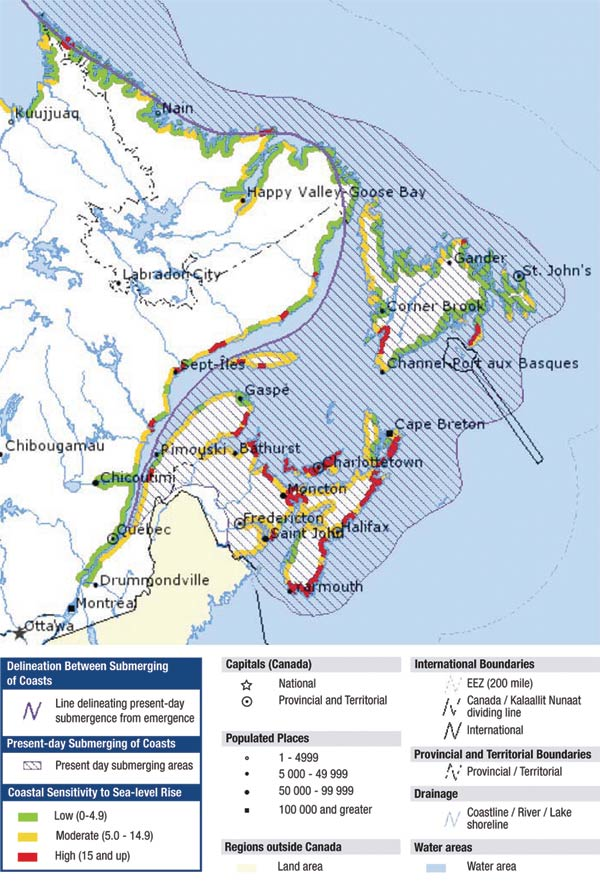
\includegraphics[height=160mm]{s3-coastalsealevel.png}
\centering
\caption{Many coastal areas in all Maritime provinces are moderately to highly sensitive to the impacts of rising sea  levels. Source: Gary Lines}
\label{fig:s3-coastalsealevel}
\end{figure}



From Vancouver to Halifax, communities across Canada face significant risks from sea-level rise and accompanying impacts.



Sea level rise from climate change is also expected to cause substantial impacts in the United States, both in exposed cities like New York and entire low-lying states like Florida.\footcite[][]{EconGetWet}
Since 2009, the U.S. Army Corps of Engineers has been incorporating sea level rise into all civil-works programs.\footcite[][]{CorpsEngSeaLevel}
Four of Florida's southernmost counties have formed the Southeast Florida Regional Climate Change Compact, which calls upon them to: ``develop a joint policy position urging the United States Congress to pass legislation that recognizes the unique vulnerabilities of Southeast Florida to the impacts of climate change''.\footcite[][]{SouthEastFloridaCompact}



In the long-term, unmitigated climate change risks causing Greenland and the West Antarctic ice sheet (WAIS) to melt.
According to the IPCC: ``Near-total deglaciation would eventually lead to a sea-level rise of around 7 m and 5 m from Greenland and the WAIS, respectively, with wide-ranging consequences including a reconfiguration of coastlines worldwide and inundation of low-lying areas, particularly river deltas''.\footcite[][See: "Deglaciation of West Antarctic and Greenland ice sheets" \url{https://www.ipcc.ch/publications_and_data/ar4/wg2/en/ch19s19-3-5-2.html}]{IPCC2007}
It goes on to say that: ``Widespread deglaciation would not be reversible except on very long time-scales, if at all''.
Recent research by the Potsdam Institute for Climate Impact Research, published in the \emph{Proceedings of the National Academy of Sciences}, concluded that for each 1˚C of temperature increase globally, sea levels may rise by 2.3 metres.\footcite[][]{PotsdamSeaLevelReport} \footcite[See also: ][]{TwoPointThreeMetres}
Sea level rise on this scale would constitute an exceptionally severe social injury --- with entire countries like Bangladesh and the Netherlands massively inundated, along with low-lying regions like Florida, New York City, and many of the world's other densely populated areas.
The IPCC identifies the ``threshold for near-total deglaciation'' at 3.2--6.2°C local warming (1.9--4.6°C global warming).
This is within the range of warming projections generated by several emission scenarios studied by the IPCC, corresponding to the absence of aggressive migitation action on the part of governments.\footcite[][See: "Projected climate change an its impacts" \url{https://www.ipcc.ch/publications_and_data/ar4/syr/en/spms3.html}"]{IPCC2007}



Sea level rise also has the potential to be abrupt: heightening the economic and human costs associated.
Recent research has concluded that during the last interglacial period ``, a critical ice sheet stability threshold was crossed, resulting in the catastrophic collapse of polar ice sheets and substantial sea-level rise''.\footcite[][p. 1]{OLeary2013}


	
	\subsubsection{Storms, droughts, and other extreme weather}



The Earth's changing climate has led to a notable rise in the number of great natural catastrophes that are driven by climate-related events over the past 25 years.\footnote{According to Munich Re, weather-related hazards can be described as a ``great natural catastrophes'' if it results in any one or a combination of the following attributes: i) number of fatalities exceeds 2,000; ii) number of homeless exceeds 200,000; iii) the country’s Gross Domestic Product (GDP) severely declines; and/or iv) the country is dependent on international aid}
Over the past 10 years, countries around the world have experienced approximately 785 natural catastrophes per year. 
During 2010 alone, a total of 950 natural catastrophes took place, nine-tenths of which were weather-related events such floods, hurricanes and storms.\footcite[][]{MunichRECatast}
Climate change is likely responsible, at least in part, for the rising frequency and severity of extreme weather events, such as floods, storms and droughts, since warmer temperatures tend to produce more violent weather patterns.\footcite[See: ][]{IPCCHurricane}
According to Environment Canada ``[f]uture warming will be accompanied by other changes, including the amount and distribution of rain, snow, and ice and the risk of extreme weather events such as heat waves, heavy rainfalls and related flooding, dry spells and/or droughts, and forest fires''.\footcite[][]{ECImpactsOfCC}



The Fourth Assessment Report of the IPCC (2007) asserts that changes in the frequency and intensity of extreme climate events will occur going into the future and will likely challenge human and natural systems to a much greater extent than natural changes in weather conditions.
These include hurricanes\footcite[][]{Knutson2004} and other extreme events including droughts, heat waves and floods.
The IPCC describes risks of extreme weather events as one of five special `reasons for concern' about climate change, along with risks to unique and threatened systems, the distribution of impacts and vulnerabilities (``those in the weakest economic position are often the most vulnerable to climate change''), aggregate impacts, and risks of large-scale singularities.\footcite[][See: "The long-term perspective" \url{https://www.ipcc.ch/publications_and_data/ar4/syr/en/spms5.html}"]{IPCC2007}
On hurricanes, the IPCC explains: ``Globally, estimates of the potential destructiveness of hurricanes show a substantial upward trend since the mid-1970s, with a trend towards longer storm duration and greater storm intensity, and the activity is strongly correlated with tropical sea surface temperature''.\footcite[][]{IPCCHurricane}
This accords with the basic science of hurricanes, which are driven by the latent heat in water vapour and gain strength from travelling over warmer water.



\begin{figure}
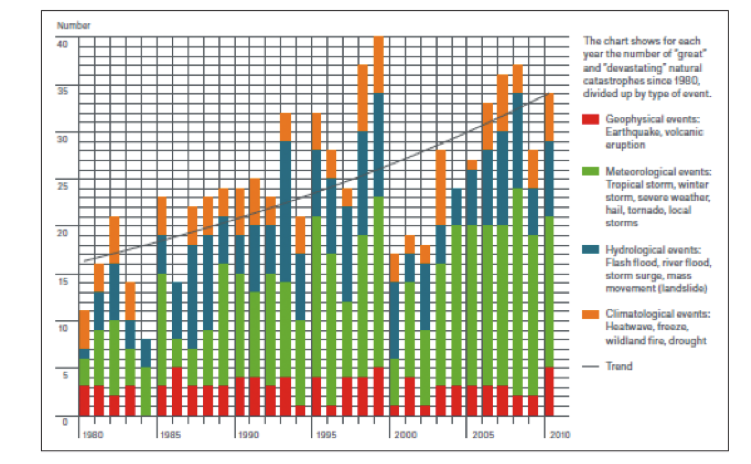
\includegraphics[width=160mm]{s3-munich-cat.png}
\centering
\caption{Global trend for great natural catastrophes since 1980. Source: Munich Re}
\label{fig:s3-munich-cat}
\end{figure}



In Canada, temperatures have warmed by an average of 0.24°C per decade, as indicated by data dating from the first official records of temperature conditions in 1948 through to 2010.\footcite[][p. 13]{TellingWeatherStory}
This figure represents twice the global average, with temperature rises in the far north occurring at rates three times faster. 
The average national temperature in 2010 reached 3.0°C above normal, making it the hottest year on nationwide records.\footcite[][p. 13]{TellingWeatherStory}



Precipitation levels in Canada have risen during the past half-century, with mean national levels increasing by about 12\%. 
This averages to about 20 more days of rain nation-wide compared with the 1950s. 
As climate change accelerates, and the rate of warming increases, the conditions for more volatile weather patterns become more common. 
Trends consistent with projections of climate models show increasing occurrence of extreme weather in Canada that can be traced back into the early 20th century. 
For instance, Figure ~\ref{fig:s3-canadadisasters} shows the increase in weather-related disasters in Canada over 100 years.



\begin{figure}
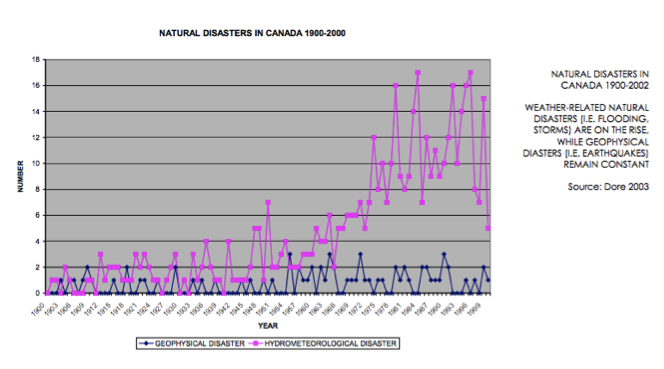
\includegraphics[width=160mm]{s3-canadadisasters.png}
\centering
\caption{Natural disasters in Canada 1900--2000. Source: Mohammed Dore, ``Forecasting the Conditional Probabilities of Natural Disasters in Canada as a Guide for Disaster Preparedness''}
\label{fig:s3-canadadisasters}
\end{figure}



By contrast, the number of geophysical disasters (earthquakes and landslides) that took place over the same time period has remained fairly consistent.\footcite[][p. 8]{ScanCCToronto}



With an influx of extreme weather come mounting costs for dealing with such events. 
In the United States, private insurers determined that 2012 was the most expensive year ever in terms of disasters linked to climate change, with a total cost of \$139 billion.\footcite[][]{BlownAway}
In Canada, the NRTEE projected that total costs associated with climate change could reach between \$21 billion and \$43 billion a year by the 2050s.\footcite[][p.15]{NRTEEPrice}
The range of estimates reflects uncertainty about the extent of action taken to reduce GHG emissions as well as other economic and population growth factors. 
Similarly, a report by the Institute for Catastrophic Loss Reduction (ICLR) for the Insurance Bureau of Canada (IBC) outlines trends of insured losses from severe weather and natural catastrophes both internationally and within Canada. 
The report reveals that financial impacts have ranged from between \$10 and \$50 billion dollars a year internationally since 2002, and with levels exceeding \$100 billion in 2011.\footcite[][p. 5]{TellingWeatherStory}
Within Canada, property insurance claims resulting from severe weather-related events from 2010-2012 have cost roughly \$1B a year.
The report outlines a number of specific examples of such claims, including:
\begin{itemize}
	\item A severe wind and thunderstorm that took place on in June of 2010 in and around Leamington in Southern Ontario caused approximately \$120 million worth of insured losses to both business and residential properties.
	\item Areas in Southern Alberta experienced a similar storm that resulted in excessive damage to private and commercial properties as well as automobiles that totalled over \$500 million in losses.
\end{itemize}
As the report details, claims resulting in both severe and smaller-impact weather events represent significant property damage for consumers, with losses driven in large part from aging sewage and water infrastructure that cannot handle the new higher precipitation levels; in fact, a rise in water levels for water-related insurance claims now ``surpass[es] fire as the number one cause of home insurance losses in many parts of the country''.\footcite[][p. 7]{TellingWeatherStory}
The report also details projections running through the 2050s of extreme weather events in Canada, including hot days per year, wildfires, hail and ice storms, tornadoes, and heavy rainfall events, and includes recommendations for dealing with the expansion of insurance-related losses nationwide.



A July 2013 study prepared by the U.S. Department of Energy examined the risks posed by climate change and extreme weather to America's energy infrastructure.
The report identifies impacts that are already being experienced, including fuel barges being impeded by low water levels in major waterways, floods and storms interfering with ports, and damage to transmission lines from storms.\footcite[][]{EnergyBreakdowns}
The report describes risks to thermoelectric power generation facilities, coastal energy infrastructure, oil and gas production, renewable energy (especially hydroelectric power), electricity transmission, fuel transport, and arctic oil and gas exploitation.\footcite[][p. I]{EnergySectorVulnerabilities}
It also concludes that: ``[i]ncreasing temperatures will likely increase electricity demand for cooling''.\footcite[][p. I]{EnergySectorVulnerabilities} \footcite[See also: ][]{USEffectsOnEnergy}



In a report for Ceres --- a  network of investors, companies, and public interest groups seeking to accelerate and expand the adoption of sustainable business practices --- Sharlene Leurig evaluated the threat of climate change to insurers.
She concluded that: ``This changing climate will profoundly alter insurers' business landscape, affecting the industry's ability to price physical perils, creating potentially vast new liabilities and threatening the performance of insurers' vast investment portfolios''.\footcite[][p. 9]{ClimateRiskInsurers}
A climate that is changing increasingly rapidly is associated with severe weather, damage to infrastructure, and soaring costs.
This corresponds with the finding of the NRTEE that ``[g]lobal mitigation leading to a low climate change future reduces costs to Canada in the long term''.\footcite[][p. 16]{NRTEEPrice}



A 2013 report from the World Meteorological Organization (WMO) described the impacts of climate change on extreme weather around the globe, concluding that ``[w]hile climate scientists believe that it is not yet possible to attribute individual extremes to climate change, they increasingly conclude that many recent events would have occurred in a different way --- or would not have occurred at all --- in the absence of climate change''.\footcite[][p. 15]{WMOExtremesReport} \footcite[See also: ][]{BBConWMO} \footcite[][]{ReutersonWMO}
WMO Secretary-General Michel Jarraud explained:
\begin{quote}
WMO's report shows that global warming was significant from 1971 to 2010 and that the decadal rate of increase between 1991-2000 and 2001-2010 was unprecedented.  Rising concentrations of heat-trapping greenhouse gases are changing our climate, with far reaching implications for our environment and our oceans, which are absorbing both carbon dioxide and heat.\footcite[][]{WMOExtremesPR}
\end{quote}
The report notes ``very large increase (more than 2000 per cent) in the loss of life from heatwaves'', as well as describing how ``Central Canada experienced its warmest and most humid summer on record in 2005. 2010 was the warmest year on record for the nation as a whole since records began in 1948.''.\footcite[][p. 6, 8]{WMOExtremesReport}



As the damage from climate change mounts, the ability of individuals and firms to mitigate the risk through insurance may diminish.
For instance, Blair Feltmate of the Climate Change Adaptation Project at the University of Waterloo projects that extreme weather arising from climate change will lead to ``an uninsurable housing market in Canada in many, many regions''.\footcite[][]{GMUninsurable}
Large-scale disasters are a particular threat to smaller insurers, given the danger that a large proportion of their policyholders may be impacted by a single extreme event.



	\subsubsection{Wildfires}
	


Increased temperatures contribute to the frequency and severity of wildfires.\footcite[][p. 33, 48, 50, 51, 53, 65 ]{IPCCar4_syr} \footcite[See also: ][]{UCSWildfire}
A 1991 study published in the \emph{Canadian Journal of Forest Research} estimated that a doubling of atmospheric \ce{CO2} would cause a 46\% increase in seasonal severity rating, with a similar increase in area burned.
A 2004 study estimated that with a doubling of \ce{CO2}, at least twice as many fires in California would ``escape'' and ``exceed initial containment limits''; that twice as large an area would be burned; and that there would be ``widespread impacts on vegetation distribution, forest condition, and carbon storage, and greatly increase the risk to property, natural resources and human life''.\footcite[][p. 169]{FriedWildfire} \footcite[See also: ][]{WesterlingWildfire}
A 2006 study of wildfire activity in the western United States found that: ``wildfire activity increased suddenly and markedly in the mid-1980s, with higher large-wildfire frequency, longer wildfire durations, and longer wildfire seasons'' and that this is ``strongly associated with increased spring and summer temperatures and an earlier spring snowmelt''.\footcite[][p. 940--943]{Westerling2006}
In the United States, the area burned annually by wildfires has grown to seven million acres, twice what it was during the 1990s.\footcite[][]{NYTFireNewNormal}
According to the Australian government's Climate Commission: ``Climate change has already increased the risk of extreme fire weather in some parts of Australia, especially the populous southeast.''\footcite[][p. 4]{CriticalDecade2013}



	\subsubsection{Increased risks to human health}



The impact of climate change on human health is no longer a contested issue, with major national and international organizations like the World Health Organization (WHO), Health Canada, the Centres for Disease Control and Prevention (CDC) and others recognizing both its existing impacts and its ongoing risks. 
The WHO, for example, asserts that ``the health effects of a rapidly changing climate are likely to be overwhelmingly negative, particularly in the poorest communities, which have contributed least to greenhouse gas emissions'' and acknowledges the increasingly damaging impact of an ever-warmer climate on numerous social and environmental health determinants, including clean air, water, food and shelter.\footcite[][]{WHOClimateHealth} \footcite[See also: ][]{LancetCCHealth} \footcite[See also: ][p. 811-7]{RacialEthnicHeat}



The negative effects of climate change on human health can be traced back almost forty years. 
For example, a 2009 WHO report entitled \emph{Global health risks: Mortality and Burden of Disease Attributable to Selected Major Risks} found that climate change since the 1970s has contributed to diarrhoea, flood injury, malaria, undernutrition, and related disease outcomes.\footcite[][p. 44]{WHOGlobalHealthRisks}
The report explains that:
\begin{quote}
Potential risks to health include deaths from thermal extremes and weather disasters, vector-borne diseases, a higher incidence of food-related and waterborne infections, photochemical air pollutants and conflict over depleted natural resources. Climate change will have the greatest effect on health in societies with scarce resources, little technology and frail infrastructure. Only some of the many potential effects were fully quantifiable; for example, the effects of more frequent and extreme storms were excluded. Climate change was estimated to be already responsible for 3\% of diarrhoea, 3\% of malaria and 3.8\% of dengue fever deaths worldwide in 2004. Total attributable mortality was about 0.2\% of deaths in 2004; of these, 85\% were child deaths. In addition, increased temperatures hastened as many as 12 000 additional deaths; however these deaths were not included in the totals because the years of life lost by these individuals were uncertain, and possibly brief.\footcite[][p. 24]{WHOGlobalHealthRisks}
\end{quote}
The WHO also states that global warming has been causing 140,000 deaths per year since 2004.\footcite[][]{WHOCCandHealth2012}
A more recent study commissioned by 20 governments around the world estimates that this number has grown to approximately 400,000 climate-related deaths per year.
The report finds that ``Climate change has already held back global development; it is already a significant cost to the global economy.''\footcite[][p. 16]{DARACVM}
The report also explains that: ``Continuing today's patterns of carbon-intensive energy use is estimated, together with climate 
change, to cause 6 million deaths per year by 2030, close to 700,000 of which would be due to climate change. This implies that a combined climate-carbon crisis is estimated to claim 100 million lives between now and the end of the next decade.''\footcite[][p. 17]{DARACVM}
According to a Health Canada assessment, the most significant impacts to human health driven by changes in climate are linked to temperature stress, extreme weather, rodent- and water-borne diseases, ultraviolet radiation, and air pollution.\footcite[][]{HHInACC} \footnote{Notably, this is one of many climate science reports produced by Canadian civil servants and essentially `buried' by the government of Stephen Harper. Planned coast-to-coast press conferences were cancelled, the report was released without publicity, and the report is not available through the Health Canada website.}
The report describes how ``the economic costs of extreme events in this country are rapidly increasing, as is the number of people affected by natural disasters'' and that ``[s]uch events and other climate-related hazards (e.g. smog, food-, water-, vector- and rodentborne diseases) continue to pose significant short- and long-term risks to the health and well-being of Canadians and their communities''.\footcite[][p. 432]{HHInACC}



It is generally accepted that the greatest impacts of ongoing climate change will be felt by people in low-income countries, as regions with weak health or governmental infrastructure will not have the capacity to respond to consequences of climate change appropriately. 
Particularly hard hit will be children, the elderly, people with illnesses or infirmities, and people with pre-existing medical conditions. 
The WHO also claims that: ``Many of the major killers such as diarrhoeal diseases, malnutrition, malaria and dengue are highly climate-sensitive and are expected to worsen as the climate changes''.\footcite[][]{WHOCCandHealth2012}
Also, a growing body of literature is drawing attention to the incommensurate impacts of climate change on vulnerable and marginalized populations.\footcite[][p. 1693--1733]{Costello2009} \footcite[][]{WHOSocialDeterm}



Rich parts of the world are also vulnerable to health effects from climate change.
The City of New York estimates that hotter summers in the 2020s ``could cause an estimated 30 to 70 percent increase in heat-related deaths, or about 110 to 260 additional heat- related deaths per year on average in New York City compared to the baseline period for the analysis (1998–2002)''.\footcite[][p. 31]{ResilientNewYork}
According to the Australian government's Climate Commission: ``Heat causes more deaths than any other type of extreme weather event in Australia. Increasing intensity and frequency of extreme heat poses health risks for Australians and can put additional pressure on health services. Changes in temperature and rainfall may allow mosquito-borne illness like dengue fever to spread south.''\footcite[][p. 4]{CriticalDecade2013}



In Canada, the relationship of health disparities to climate change impacts and adaptation is a newly emerging area of study. 
Recent reports predict that hotter city temperatures will lead to between five and 10 additional deaths per 100,000 people per year by 2050 as well as contribute to increasing pressure on Toronto hospitals due to sickness and other heat-related conditions that could swell associated costs to between \$3 million to \$8 million annually by the 2050s.\footcite[][p. 87]{NRTEEPrice}
The NRTEE concluded that climate change ``will lead to warmer summers and poorer air quality, resulting in increased deaths and illnesses in the four cities studied — Montréal, Toronto, Calgary, and Vancouver'' and that this will impose costs on the health care system of between \$3 million and \$11 million per year by the 2050s.\footcite[][p. 16]{NRTEEPrice}



	\subsubsection{Ecosystem collapse}



Climate change is expected to have a substantial effect on ecosystems and biodiversity around the world.\footcite[][p. 1]{VulnerableSpecies}
Writing in \emph{Nature Climate Change}, a group of researchers concluded that ``without mitigation, large range contractions can be expected even amongst common and widespread species, amounting to a substantial global reduction in biodiversity and ecosystem services by the end of this century''.\footcite[][p. 1]{WarrenBiodiversity}
Because ecosystems are vital to the survival and prosperity of humanity, climatic damage imposed on them is an important form of social injury arising from the activities of fossil fuel companies.
As emphasized by the United Nations Development Programme, the link between ecosystem integrity and prosperity is especially important for the poor: ``Climate change is already exacerbating chronic environmental threats, and ecosystem losses are constraining livelihood opportunities, especially for poor people.''\footcite[][p. 95]{UNHumanDev2013}



Salmon provide just one example of an important species that faces threats from climate change. 
The dangers climate change poses to salmon are illustrative for a number of reasons: these fish serve as an extension of the discussion relating to threats to Canadian coastal environments described above; salmon fisheries in particular are significant contributors to the global economy and to the subsistence of large segments of the world’s populations; and salmon play a critical role in the functioning of their marine ecosystems.



A report from the International Union for Conservation of Nature (IUCN) that the salmon fishing industry contributed more than \$2 billion to economies in Russia, Japan, the U.S., and Canada and directly employed more than 35,000 people.\footcite[][p. 2]{IUCNSalmon}
Salmon are also harvested on a smaller scale, both for recreational and subsistence purposes.
Many individuals, communities and small businesses are dependent on salmon to sustain their livelihoods and to provide a significant contribution of their diet. 
Reliance on salmon fisheries as both a source of food and income is especially important to communities along Canada's Atlantic and Pacific coasts. 


In 2009, the IUCN released ``Red List of Threatened Species: More Than Just the Polar Bear'', highlighting the need to more closely study the complex risks associated with climate change to delicate ecosystems and the species that inhabit them.\footcite[][]{IUCNMorePolarBear}
The report includes a detailed discussion about the problems that increasing global temperatures will pose to the safety of the world's salmon populations. 
For instance, with respect to the role of this species in their natural environment, salmon provide food for a suite of predators and scavengers that live along the coasts of the ocean and beside the banks of streams and rivers that they traverse as part of their extensive migratory routes. 
Animals such as seals, whales, otters, bears, birds, and many invertebrates feed on salmon, many at critical stages in their own yearly feeding cycles, as a vital source of protein and fat. 
Furthermore, throughout a salmon's life cycle, it will transport essential nutrients from saltwater to freshwater areas as well as to the surrounding lands via the excretion of waste as well as through the decay of carcasses.



Increases in water temperatures concurrent with rises in global air temperatures impose a number of negative effects on salmon. 
Direct biological impacts include increased physiological stress, susceptibility and exposure to disease, and challenges and disruptions to breeding. 
These effects on the biology of salmon may potentially lead to impacts in the long-term. 
For example, because the development of salmon relies on water temperature, warmer waters could result in early migration of juvenile fish. 
Because natural patterns are timed with other important feeding phenomena such as planktonic blooms, early migrations could mean an insufficient source of food for salmon entering the oceans at a critical point in their development. 
Similarly, flows of warm freshwater can create thermal barriers to migrating salmon, requiring additional energy to navigate. 
Such barriers can also delay or even prevent spawning altogether. 
Moreover, increased winter flows can damage river beds, as well as the nests of salmon eggs dug into the sediment and gravel.



Warmer ocean temperatures have also been shown to reduce the abundance of other smaller fish into certain areas experiencing an influx of new warmer waters. 
Because the interaction of the multitude of biological factors that play a role in maintaining the balance of healthy ecosystems, scientists are hard-pressed to forecast specific predictions, let alone detail recommendations for large-scale strategies to deal with potential climate-related threats to salmon, as well as for the increasing range of at-risk species. 
Acceleration of climate change will exacerbate these difficulties, and can have profound environmental as well as economic impacts. 
The only sure means of maintaining the health of terrestrial and aquatic ecosystems is to significantly mitigate the release of greenhouse gas emissions into the atmosphere.



At the same time as they increase global temperatures, heightened \ce{CO2} concentrations in the atmosphere cause the oceans to become more acidic.
According to the IPCC, this is ``expected to have negative impacts on marine shell-forming organisms (e.g. corals) and their dependent species''.\footcite[][p. 52]{IPCCar4_syr}
The IPCC also expects ocean acidification to be part of a suite of changes that that makes it ``likely'' that ``[t]he resilience of many ecosystems'' will be ``exceeded this century''.\footcite[][p. 48]{IPCCar4_syr}
A 2010 report from the United Nations Environment Programme concluded that: ``[i]f ocean acidification continues 
disruptions to food chains and direct and indirect impacts on numerous species are considered likely with consequent risk to food security''.\footcite[][p. 8]{UNEPOceanAcid} \footcite[See also: ][]{AcidThreatFish}
The report suggests that: ``[t]he obvious solution to the potential threats posed by ocean acidification is to make rapid and substantial cuts to anthropogenic \ce{CO2} emissions to the atmosphere''.\footcite[][p. 8]{UNEPOceanAcid}
Canada's Department of Fisheries and Oceans has also highlighted the danger of ocean acidification.
In a 2013 report, they attribute the phenonemon's ``unprecedented rate of occurrence'' to ``the significant amount of carbon dioxide that has been added to the atmosphere over the past 250 years''.\footcite[][p. 4]{FaOAcid}
They further explain that:
\begin{quote}
The potential effects of ocean acidification include altered seawater chemistry; decreased growth and productivity of calcium carbonate-based organisms; changes in respiration in large invertebrates, fish, and some zooplankton; increased growth of certain seaweeds and sea grass; changes in species composition and dominance; societal and economic impacts; and other potential impacts that presently remain unknown.\footcite[][p. 6]{FaOAcid}
\end{quote}
The report describes biophysical impacts on nutrients and toxicity, marine organisms, benthic invertebrates, marine fish, seaweed and sea grade, and ecosystem structure and function, along with socioeconomic impacts on marine fisheries and marine aquaculture.\footcite[][p. 13]{FaOAcid}



Because of both warming and the acidification of the world's oceans in response to rising \ce{CO2} concentrations, coral reefs are especially vulnerable to climate change.
In their fourth assessment report, the IPCC concluded that increased coral bleaching would accompany warming of 1˚C, most corals will be bleached above 1˚C, and ``widespread coral mortality'' is expected above 2.5˚C.\footcite[][p.51]{IPCCar4_syr}
Significant damage to coral reefs has already been observed, including the loss of 50.7\% of initial coral cover in Australia's Great Barrier Reef.\footcite[][]{27declinecoral}
Caribbean corals are also experiencing record thermal stress, bleaching, and mortality.\footcite[][]{CaribbeanCorals}
An article in \emph{Science} explains that: ``Atmospheric carbon dioxide concentration is expected to exceed 500 parts per million... by 2050 to 2100, values that significantly exceed those of at least the past 420,000 years during which most extant marine organisms evolved''.\footcite[][p. 1737--1742]{CoralRapidCC}
It concludes that: ``[t]he result will be less diverse reef communities and carbonate reef structures that fail to be maintained''.\footcite[][p. 1737--1742]{CoralRapidCC}
As exceptionally rich ecosystems, coral reefs have an importance that goes beyond their inherent biological value.
Ecosystem services provided by coral reefs, including food, jobs, and tourism, have an estimated value of as much as \$375 billion per year.\footcite[][]{NOAACoral}



Many other species are expected to experience negative impacts from climate change.
For instance, reductions in sea ice ``will drastically shrink marine habitat for polar bears, ice-inhabiting seals, and some seabirds, pushing some species toward extinction'' while ``caribou/reindeer and other land animals are likely to be increasingly stressed as climate change alters their access to food sources, breeding grounds, and historic migration routes''.\footcite[][Executive summary, p. 10]{ACIA2004}
One 2013 study found that ``608–851 bird (6–9\%), 670–933 amphibian (11–15\%), and 47–73 coral species (6–9\%)'' are ``highly climate change vulnerable''.\footcite[][p. 1]{VulnerableSpecies}
A 2013 study from BirdLife International found that ``[c]limate change is already affecting birds in diverse ways]'', and that ``[m]any species will suffer from range shifts and losses, and some will become extinct'' as a result.\footcite[][p. 15]{StateWorldBirds} \footcite[See also: ][]{CBCBirdLife}
The report also highlights how the risks to birds increase as temperature increase exceeds 2˚C: ``[t]emperature rises beyond this level are predicted to lead to catastrophic extinction rates, with few management options''.\footcite[][]{BirdLifeCC}



An Environment Canada briefing released under the \emph{Access to Information Act} argues that ``[h]ealthy and resilient ecosystems are one of our best defences against a changing climate'' and states that more than 13\% of Canada's gross domestic product depends on healthy ecosystems.\footcite[][]{CanadaEcosystemBriefing}
The document identifies climate change as one of ``several major threats'' that are causing ``significant biodiversity loss''.




Considerable scope exists for reducing the degree of ecosystem damage resulting from climate change by reducing future greenhouse gas pollution emissions.
The article in \emph{Nature Climate Change} concludes that: ``without mitigation, $57 \pm 6\%$ of plants and $34 \pm 7\%$ of animals are likely to lose $\ge 50\%$ of their present climatic range by the 2080s. With mitigation, however, losses are reduced by 60\% if emissions peak in 2016 or 40\% if emissions peak in 2030''.\footcite[][]{WarrenBiodiversity}



	\subsubsection{Threats to First Nations groups and indigenous cultures}



Climate change threats to northern Canadian provinces, as well as the Aboriginal communities that live there, are becoming increasingly recognized. 
For example, Natural Resources Canada's recently published national assessment ``From Impacts to Adaptation: Canada in a Changing Climate 2007'' states explicitly that ``resource-dependent and Aboriginal communities are particularly vulnerable to climate changes'', and emphasizes that ``vulnerability'' to climate change risk is ``magnified in the Arctic.''\footcite[][p.3, p. 14]{ImpToAda} 
Similarly, the Arctic Council and the International Arctic Science Committee (IASC) issued a report in 2004 entitled the ``Arctic Climate Impact Assessment'' that aimed  to synthesize knowledge on climate variability and to assess and predict the impact of climate change on arctic regions and communities going into the future.\footcite[][]{ACIA2004}
The report contains contributions from over 300 scientists, professionals, and Aboriginal community leaders and reveals that future climate change could be devastating for numerous Inuit communities.
These findings are supported by a more recent study conducted by researchers from McGill University that focused on two separate Inuit communities.\footcite[][]{CCInuitCommunities}
The study identifies that ``climatic conditions which currently pose risks are expected to be negatively affected by future climate change'' and explains that ``young Inuit and those without access to economic resources, in particular, are vulnerable''.\footcite[][p. 45, p. 54]{CCInuitCommunities}



According to a 2009 article in \emph{Global Environmental Change}, ``health inequality [in relation to climate change] is
particularly pronounced among Aboriginal Canadians''.\footcite[][p. 1]{VulAborig2009}
While climate change in general ``has been identified as potentially the biggest health threat of the 21st century'', the article goes on to explain that ``[t]he existing burden of ill-health increases the sensitivity of Indigenous peoples to the adverse impacts of climate change, which combined with a proportionally higher dependence of many Indigenous livelihoods on the environment, spiritual and cultural ties to the land, demographic trends, and experience of marginalization, makes Indigenous peoples particularly vulnerable''.\footcite[][p. 1]{VulAborig2009}



	\subsubsection{Threats to the infrastructure of cities, including Toronto}



More than half the world's population live in cities and urban areas. 
As a first step towards addressing climate change, many cities have conducted assessments of their GHG emissions, as well as begun to evaluate their vulnerability to climate change impacts.
The City of New York projects that --- because of rising sea levels and ocean temperatures --- by 2050 ``a storm like [Hurricane Sandy could cause an estimated \$90 billion in losses (in current dollars) --- almost five times as much''.\footcite[][Foreward, p. 2]{ResilientNewYork}



In Canada, over 200 municipalities are taking part in the Partners for Climate Protection  program, which is the Canadian component of International Council for Local Environmental Initiatives's Cities for Climate Protection network.\footnote{See: \url{http://www.icleicanada.org/programs/mitigation/pcp}}
The Province of Ontario and the City of Toronto are among those actively implementing numerous plans and initiatives to reduce GHG pollution. 
The first attempt on behalf of the City to assess GHG levels came in 2004.\footcite[][p. IV]{GHGPollutionToronto}
Follow-up reports detailing strategies for reducing emissions were published soon after.\footcite[][]{CCAHealthEquity}
Additionally, there is a growing body of literature that examines current trends and anticipated affects of climate change to Toronto and surrounding areas.\footcite[][]{TorontoEnvOff2007} \footcite[][]{TorontoAheadStorm} \footcite[][]{ScanCCToronto} \footcite[][]{AdaptPrioritiesCanada} \footcite[][]{MacLeodAdaptation}



It is now generally recognized that impacts of climate change are already being felt in Toronto and the GTA.
Toronto has experienced extreme heat, floods, droughts, new insect pests, new vector-borne diseases and other problems worsened by climate change.\footcite[][]{TorontoAheadStorm}
In terms of fluctuations to regular weather patterns, Toronto has seen an average temperature increase of 2.7°C since the late 1800s.\footcite[][p. 5]{ScanCCToronto}



Record high temperatures, accompanied by smoggier skies, have also been recorded in recent summer seasons. 
For instance, 2005 saw the warmest June on record: 37 days had a maximum temperature greater than 30°C (more than double the average from 1971-2000); humidex values exceeded 35 more than 44 times; and 48 smog days were declared, the highest number on record.\footcite[][p. iii, p. 7]{ScanCCToronto}
While precipitation patterns have not undergone such drastic changes, it has been predicted that precipitation will likely arrive during heavy rainfall events. \footcite[][p. 6]{ScanCCToronto}
For instance, snowfall is expected to decrease and rainfall will increase in its stead, accompanied by an influx of freezing rain episodes.\footcite[][p. 8]{TorontoAheadStorm}
More ice-storms are also expected.\footcite[][]{FreezingRain2007}
More freeze-thaw cycles in the city are also projected, which take a heavy toll on roads as well as urban green spaces.\footcite[][p. 8]{TorontoAheadStorm}



\textbf{Increased financial burdens on the city}



High density cities such as Toronto are particularly susceptible to damage caused by extreme weather or natural disasters. 
Extreme weather events driven by climate change can also be costly for municipalities, financially as well as in terms of lives lost and damage to cultural assets. 
For example, the intense storm that took place in the city on August 19, 2005 caused millions of dollars of damage. 
This storm's heavy rainfall washed out a part of Finch Avenue, and caused flash flooding and widespread damage across the city. 
Parks and Recreation spent \$12.5 million restoring damaged trees and urban parks. 
\$600,000 was spent by Urban Forestry Services to clear fallen trees.\footcite[][p. iii]{ScanCCToronto}
Likewise, Transportation Services spent close to \$5 million repairing Finch Avenue. 
The total damage, including public and private property, was estimated at approximately \$400 -- \$500 million --- the most expensive storm in Toronto's history.\footcite[][p. 11]{TorontoAheadStorm}



More frequent storms and severe weather will likely continue to cause damage to city infrastructure and put strain on city resources. 
Indeed, the floods, storms, droughts and other weather-related phenomena that already occur annually in Canada can cost hundreds of millions of dollars.\footcite[][p. 11]{HHInACC}
Furthermore, recent events such as Hurricane Sandy have revealed that even developed countries can be devastated by extreme weather events that are difficult to prepare for and which can be unprecedented in terms of strength and geographic scope.   



\textbf{Increased health risks to vulnerable populations}



While severe storms and extreme weather can be very costly, the longer-term  impacts of climate change will have an adverse affect on the city and its residents in ways that ``[go] well beyond the reported monetary costs''.\footcite[][p. 19]{CCAHealthEquity}
It is widely documented that certain populations in a particular city are more vulnerable to the adverse affects of climate change than others.\footcite[][]{EbiHealthJustice} \footcite[][]{HotWeatherResponse2006} \footcite[][p. 1153--1163]{MarmotHealthOutcomes} \footcite[][]{ReducingHealthDisparities}
`Vulnerability' in this sense can be defined as ``the degree to which individuals and systems are susceptible to or unable to cope with the adverse effects of climate change''.\footcite[][p. 6]{CCAHealthEquity}
Determinants of health, such as income and social status, education and literacy, social and physical environments, or genetics, etc., can be used to assess a population's vulnerability to the various impacts of climate change. 
For example, severe storm events can affect physical environments by causing extensive property damage; challenges linked with income and social status can be reinforced as those with inadequate employment or insufficient funds could have more difficulty acquiring financial resources to repair property, deal with displacement, or finance interim accommodation. 
Populations that are particularly vulnerable to climate change impacts in the City of Toronto, include infants and babies, women, the elderly, those with preexisting or underlying conditions, First Nations, those whose livelihood is reliant on natural resources, and those with low social and economic standings.\footcite{CCAHealthEquity} \footcite[][]{HHInACC} \footcite[][]{HealthCanadaPreparingImpacts}



The current and forecasted future makeup of the City of Toronto is one that is both highly diverse and increasingly expanding; indeed, the population of the Greater Toronto Area is estimated to reach 9.2 million by 2036.\footcite[][]{DemoProjections2012}
Toronto's swelling population encompasses a number of the vulnerable populations identified above. 
For instance, according to Statistics Canada, the First Nations population of the city grew 20\% from 2001, reaching a total of 13,605 people as of 2006.\footcite[][]{2006TorontoProfile}
This figure represents over 0.5\% of the total population in the City, and 43\% of the First Nations population in the Greater Toronto Area (GTA). 
Moreover, Statistics Canada reports that the City of Toronto was home to over 350,000 seniors in 2006.
This number constitutes 14\% of the City’s population, and 53\% of all seniors living in the GTA. 
The city's Social Development, Finance and Administrative Division forecasts that seniors will make up 17\% of the City of Toronto population by 2031.\footcite[][p. 5]{SeniorsDemographicSnapshot}
Finally, an increasing number of Torontonians are low-income.
For instance, in 2005 there were 134,247 family households and 165,156 persons not living in family households that reported before-tax income levels below Statistics Canada's Low Income Cut-off.\footcite[][p. 5]{LowIncomeProfile}
The size of the low-income population recorded in 2005 was greater than in the early 1990s, and represents almost double the size as in the rest of the GTA.\footcite[][p. 6]{LowIncomeProfile}



The literature on health equity in a Canadian context shows a direct relationship between health and income.\footcite[][]{HotWeatherResponse2006} \footcite[][]{PovertyMakingSick} \footcite[][]{PovertyInequalityHealth}
People living in poor areas in Toronto experience increased risk factors for illness, higher occurrence of disease, and early mortality than people who reside in more affluent areas.
Such risks will very likely be aggravated by the impacts of climate change on the city.
A Waterloo-based study exploring the connection between effects of climate change and the homeless population found that exposure to extreme weather was high for this segment of the population; furthermore, exposure exacerbated pre-existing illnesses such as drug and alcohol addictions, mental illness, cardiovascular and respiratory conditions, as well as feelings of isolation and increased stress.\footcite[][]{HomelessnessWaterloo}



A more comprehensive examination of the various ways that the City of Toronto will suffer social, economic, and environmental injury as a direct result of climate change can be found in the 2009 Clean Air Partnership Report ``Climate Change Adaptation and Health Equity''.\footcite[][]{CCAHealthEquity}
It includes details about the affect of impacts on Toronto's water supply and water quality, energy sources, transportation sector and services, buildings and infrastructure, urban ecosystem, tourism, and economy.  



	\subsubsection{Abrupt and non-linear adverse climate impacts}



The Earth's climate system includes some powerful positive feedback mechanisms capable of multiplying the climate-altering effect of greenhouse gases.
These include the way in which melting ice decreases the planet's albedo (reflectiveness), causing more of the sun's energy to be directed toward increasing temperatures.
Other feedback mechanisms include the release of methane --- a powerful greenhouse gas --- from melting permafrost and subsea methane clathrate deposits.\footcite[See: ][]{VastCostsArctic} \footcite[See also: ][]{Thermokast2013} \footcite[See also: ][]{VidalTimebomb}
Abrupt methane release has been associated with past instances of abrupt global warming, such as during the Paleocene–Eocene Thermal Maximum 55 million years ago, and several of these instances were accompanied by major global extinction events both on land and in the oceans.\footcite[See: ][]{Hansen2010}
According to NASA:
\begin{quote}
Over hundreds of millennia, Arctic permafrost soils have accumulated vast stores of organic carbon --- an estimated 1,400 to 1,850 petagrams of it (a petagram is 2.2 trillion pounds, or 1 billion metric tons). That's about half of all the estimated organic carbon stored in Earth's soils. In comparison, about 350 petagrams of carbon have been emitted from all fossil-fuel combustion and human activities since 1850. Most of this carbon is located in thaw-vulnerable topsoils within 10 feet (3 meters) of the surface.\footcite[][]{SleepingGiant}
\end{quote}
NASA also explains that: ``Permafrost soils are warming even faster than Arctic air temperatures ... 1.5 to 2.5 degrees Celsius in just the past 30 years'' and that this warming ``threatens to mobilize these organic carbon reservoirs and release them into the atmosphere as carbon dioxide and methane, upsetting the Arctic's carbon balance and greatly exacerbating global warming''.\footcite[][]{SleepingGiant}



Several potentially dangerous `tipping points' have been identified by scientists, including the danger that the themohaline circulation which produces Europe's relatively warm climate relative to its latitude may be disrupted, though this is now considered unlikely, at least within the next century.\footcite[][]{IPCCThermohaline}
Writing in \emph{Nature} in 2009, Johan Rockstrom et al. explain that:
\begin{quote}
We propose that human changes to atmospheric \ce{CO2} concentrations should not exceed 350 parts per million by volume, and that radiative forcing should not exceed 1 watt per square metre above pre-industrial levels. Transgressing these boundaries will increase the risk of irreversible climate change, such as the loss of major ice sheets, accelerated sea level rise and abrupt shifts in forest and agricultural systems. Current \ce{CO2} concentration stands at 387 p.p.m.v. and the change in radiative forcing is 1.5 W $m^{−2}$.\footcite[][]{SafeOperatingSpace}
\end{quote}
In their Fourth Assessment Report, the IPCC explains that ``[a]nthropogenic warming could lead to some impacts that are abrupt or irreversible'', including in the form of ``metres of sea level rise'', ``significant extinctions'' (40 to 70\% of species assessed if warming exceeds 3.5˚C), and ``[c]hanges in terrestrial and ocean \ce{CO2} uptake [that] may feed back on the climate system''.\footcite[][p. 53]{IPCCar4_syr}



The climate system has experienced dramatic changes in the past, such as the Permian–Triassic extinction event.
This event, which took place 252 million years ago, saw 96\% of marine species and 70\% of terrestrial species become extinct, and took as long as 10 million years to recover from.\footcite[][p. 759--765]{PTRecovery}
Possibly caused by volcanism, this event involved ``global warming by 6˚C and huge input of light carbon into the ocean-atmosphere system'' and ``an ever-worsening positive-feedback loop, the `runaway greenhouse'.''\footcite[][p. 358]{EndPermian}
It is possible that human GHG pollution on a significant scale could induce massive additional GHG release as permafrost and clathrates melt, and as forests dry out and burn.
A severely amplified anthropogenic greenhouse effect could pose a significant danger to human civilization and many forms of life on Earth.



The planet Venus may have experienced a `runaway' climate change scenario.
Beginning in a state where liquid water existed on its surface, as the result of the sun growing brighter over long periods of time Venus experienced an accumulation of water vapour and \ce{CO2} in its atmosphere.\footcite[][]{VenusRunaway}
Now the surface of the planet has an average temperature of 462˚C.
NASA climatologist James Hansen has suggested that the Earth could experience a runaway greenhouse effect and adopt a climate like that of Venus if fossil-fuel use continues until reserves are exhausted.\footcite[][p. 22-23]{HansenVenusThreat}
Research published in \emph{Nature Geoscience} in July 2013 concluded that the threshold for such runaway warming may be lower than previously estimated.\footcite[][]{Goldblatt2013}



	\subsubsection{Security implications}
	
	
	
A number of major analyses have been focused on the likely global security implications of climate change.
In 2008, a National Intelligence Assessment was assembled by 16 U.S. intelligence agencies.
While the report is classified, the chairman stated publicly that climate change could disrupt U.S. access to raw materials, create millions of refugees, and cause water shortages and damage from melting permafrost.\footcite[][]{Craven}
A 2003 report commissioned by the Pentagon considered some of the more dramatic possible warming scenarios and concluded that:
\begin{quote}
In short, while the US itself will be relatively better off and with more adaptive capacity, it will find itself in a world where Europe will be struggling internally, large number so [sic] refugees washing up on its shores and Asia in serious crisis over food and water. Disruption and conflict will be endemic features of life.\footcite[][p. 22]{AbruptCCScenario}
\end{quote}
It also argues that: ``with inadequate preparation, the result [of abrupt climate change] could be a significant drop in the human carrying capacity of the Earth’s environment''.\footcite[][p. 1]{AbruptCCScenario}
A report prepared for the Center for Naval Analysis --- produced by a ``blue-ribbon panel of retired admirals and generals from the Army, Navy, Air Force, and Marines'' --- calls climate change ``potentially devastating''.\footcite[][p. 3]{NationalSecurityCC}
A joint report from the Center for Strategic and International Studies and the Center for a New American Security describes how current projections from climate models are ``too conservative'' and that ``at higher ranges of the [warming] spectrum, chaos awaits''.\footcite[][p. 78]{AgeOfConsequences}
The report also highlights the need for urgent action to reduce emissions: ``An effective response to the challenge of global warming cannot be spread out across the next century, but rather must be set in place in the next decade, in order to have any chance to meaningfully alter the slope of the curves one sees in the IPCC report''.\footcite[][p. 78]{AgeOfConsequences}



In 2012, the U.S. National Academy of Sciences published a report on: ``Climate and Social Stress: Implications for Security Analysis''.\footcite[][]{SocialStress}
The report concludes that:
\begin{quote}
Anthropogenic climate change can reasonably be expected to increase the frequency and intensity of a variety of potentially disruptive environmental events— slowly at first, but then more quickly. Some of this change is already discernible. Many of these events will stress communities, societies, governments, and the globally integrated systems that support human well-being.\footcite[][p. S-2]{SocialStress}
\end{quote}
And that:
\begin{quote}
It is prudent to expect that over the course of a decade some climate events—including single events, conjunctions of events occurring simultaneously or in sequence in particular locations, and events affecting globally integrated systems that provide for human well-being—will produce consequences that exceed the capacity of the affected societies or global systems to manage and that have global security implications serious enough to compel international response. It is also prudent to expect that such consequences will become more common further in the future.\footcite[][p. S-4]{SocialStress}
\end{quote}
All told, the report describes in great detail the ways in which climate change is a national security issue for the United States, as well as a threat to international peace and security.


In March 2013, Admiral Samuel J. Locklear III --- the chief of U.S. naval forces in the Pacific --- argued that climate change ``is probably the most likely thing that is going to happen... that will cripple the security environment, probably more likely than the other scenarios we all often talk about''.\footcite[][]{PacificChiefWorry}



A 2013 article published in the journal of the Royal United Services Institute describes how climate change could contribute to global instability by exposing cities to extreme events.
It also raises concerns about unforeseen social and political consequences from adaptation and mitigation, as well as the possibility of geoengineering.\footcite[][]{DalbyCCSecurity}



In a 2010 study conducted by the Canadian Department of National Defence (DND), climate change was identified as one reason why ``[t]he maritime domain... will become increasingly contested over the coming years and decades''.\footcite[][p. 25]{SinkingFeeling}
In 2012, officials from the Canadian Security and Intelligence Service and DND attended a briefing on the security risks posed by climate change.\footcite[][]{CCSecurityBriefing}
The presentation --- which has been declassified for release through access to information legislation --- described climate change impacts including extreme weather events, impacts on coastal cities, damage to food security, and loss of biodiversity.



	\subsection{The harm caused is inherent to the primary business of fossil fuel companies}



All the social injuries described above are imposed on innocent parties by fossil fuel companies in the course of their fundamental business activity of extracting coal, oil, and gas.
These harms are inseparable from the continuation and expansion of these core business activities.
According to the Government of Canada, 80\% of Canada's GHG emissions arise from the ``production or consumption of fossil fuels for energy purposes''.\footcite[][]{GoConGHGs}
As a result, shareholder voice is not an effective strategy for mitigating these harms.
The University of Toronto's investments in these companies increase the amount of harm that will arise as a result of climate change.



Divestment is the only way for the University of Toronto to avoid contributing financially to the fossil fuel industry, and by extension, to the socially injurious impacts delineated above.
Besides divestment, another approach to socially responsible investment is to try to alter a firm’s behaviour by applying pressure through shareholder voice. 
However, the harmful activities (extracting and selling fossil fuels) are inherent to the primary business of fossil fuels companies in which the university is invested.  
In this sense, investments in fossil fuel companies closely parallel investments in tobacco companies; in both cases, the problem is the primary product being produced by the industry.



For example, Shell Canada lists its business activities as follows: ``Shell Canada's Upstream businesses explore for and extract natural gas, and market and trade natural gas and power. Our Downstream business refines, supplies, trades and ships crude oil worldwide and manufactures and markets a range of products, including fuels, lubricants, bitumen and liquified petroleum gas (LPG) for home, transport and industrial use.''\footcite[][]{ShellAtAGlance}
ExxonMobil describes its upstream and downstream activities similarly.\footcite[][]{ExxonWhatWeDo}



Given the centrality of oil and natural gas extraction, as well as the refinement and sale of these resources to the business models of these companies, shareholder voice would not be an effective method to address social injury since the companies could not abandon the socially injurious activity without dissolving their existing business models.  
Moreover, the market value of these companies reflects an assumption that their reserves will be extracted and burned.  
Therefore, it would be unreasonable for the University of Toronto to expect to be able to alter the socially injurious activities of these companies while holding onto its investments in the fossil fuel industry.  
Thus, divestment is the only appropriate response for the University of Toronto to adopt in order to dissolve any financial complicity in the fossil fuels industry’s socially injurious activities.  



	\subsection{The business activities of these companies frustrate the enforcement of the rules of domestic and international law intended to protect individuals against deprivation of health, safety, and basic freedoms}
	\label{sec:FrustrateLaw}



The socially injurious activities of fossil fuel companies frustrate the enforcement of rules of domestic and international law intended to protect individuals against deprivation of health, safety and basic freedoms.  
This includes the violation of specific domestic and international statutes, the violation of common law duties such as through the creation of nuisance, and the frustration of international diplomatic efforts to address climate change.



	\subsubsection{Canadian domestic law}


\begin{vcom}
Insert summary paragraph, once other text finalized
\end{vcom}



At the highest level, the activities of fossil fuel companies risk undermining the \emph{Canadian Charter of Rights and Freedoms}.  
Section 7 states: ``the right to life, liberty and security of the person and the right not to be deprived thereof except in accordance with the principles of fundamental justice''.\footcite[][]{CharterRF}
Arguably, the harms associated with climate change could become so substantial as to deprive people of these rights.
In particular, that could be the case for particularly vulnerable populations and communities within Canada, such as small northern settlements.
Settlements built on permafrost could become too dangerous to inhabit, while those dependent on ice roads for supplies could become too isolated to be economically viable.
Further, if the sea level rise projections discussed in \nameref{sec:inundationcoastal} prove justified, the security of the person and lives of many people across Canada could be threatened.



The activities of the fossil fuels industry in Canada also violate the constitutional and treaty rights of Canada's First Nations.
These violations arise both from the specific impact of fossil fuel development projects --- such as the oil sands --- and from the inevitable consequences of burning fossil fuels.
Rights that are being violated include the right to consultation and accommodation; the right to fish, hunt, and trap; and the aboriginal rights affirmed in Canada's constitution.
Keepers of the Athabasca member Vivienne Beisel explains how the oil sands development has violated Treaty 8 and the constitution:
\begin{quote}
The cumulative impacts of oil sands development has all but destroyed the traditional livelihood of First Nations in northern Athabasca watershed. The law is clear that First Nations must be consulted whenever the province contemplates action that may negatively affect Aboriginal and treaty rights... The province has continued to issue approvals for new developments without obtaining their consent or consulting with First Nations in a meaningful and substantial way. This is in direct breach of Treaty 8 First Nations' treaty-protected Aboriginal rights to livelihood, and thus a violation of s.35(1) of the Constitution.\footcite[][]{PassingNoNewOilSandsApprovalsResolution}
\end{quote}
In June 2013, the Lac La Biche-area Cree won a case at the Court of Appeal of Alberta allowing them to proceed with a lawsuit against the Canadian federal government and the Government of Alberta.
The Cree allege that the cumulative impacts of 300 operating oil sands projects impact their rights to hunt and fish under Treaty 6.\footcite[][]{BandWinsTreatyRights}
560,000 barrels of oil per day are being extracted from the territory in question --- 30\% of the total output from the oil sands.
Future projects that have been announced would increase that total to 1.6 million barrels per day.



Analysis from the Pembina Institute highlights some of the ways in which oil sands expansion is especially damaging, including in terms of land disturbance, air quality, water use, greenhouse gas emissions, and the production of tailings.\footcite[][p. 1]{PembinaOilsandsExpansion}
Each of these impacts has both direct and indirect effects on aboriginal communities, ranging from the contamination of local water supplies to the general worsening of climate change.
The oil sands are the fastest-growing source of GHG pollution in Canada, undermining Canada's domestic climate change objectives and reducing the chances of the world as a whole keeping the degree of warming below the accepted safe level.



One of the most comprehensive analyses of environmental incidents associated with the oil sands demonstrates how numerous violations of environmental regulations have been since 1996, as well as how rarely they have led to enforcement action.
In a peer-reviewed report prepared for Treeline Ecological Research and Global Forest Watch Canada, Kevin Timoney and Peter Lee found that over 4,000 alleged contraventions of regulations took place in Canada's oil sands between 1996 and 2012.\footcite[][p. 8]{OnePercentReport} \footcite[See also: ][]{GlobalFewerOnePercent} \footcite[See also: ][]{FinPoOnePercent}
Syncrude's Mildred Lake operation and Suncor were collectively responsible for 86.6\% of these contraventions.\footcite[][p. 8]{OnePercentReport}
During the time period under consideration, Alberta's environment ministry only took action to enforce regulation in 37 cases, representing 0.9\% of the total.
In cases where enforcement action was taken, the mean penalty was \$4,500.



\begin{figure}[h]
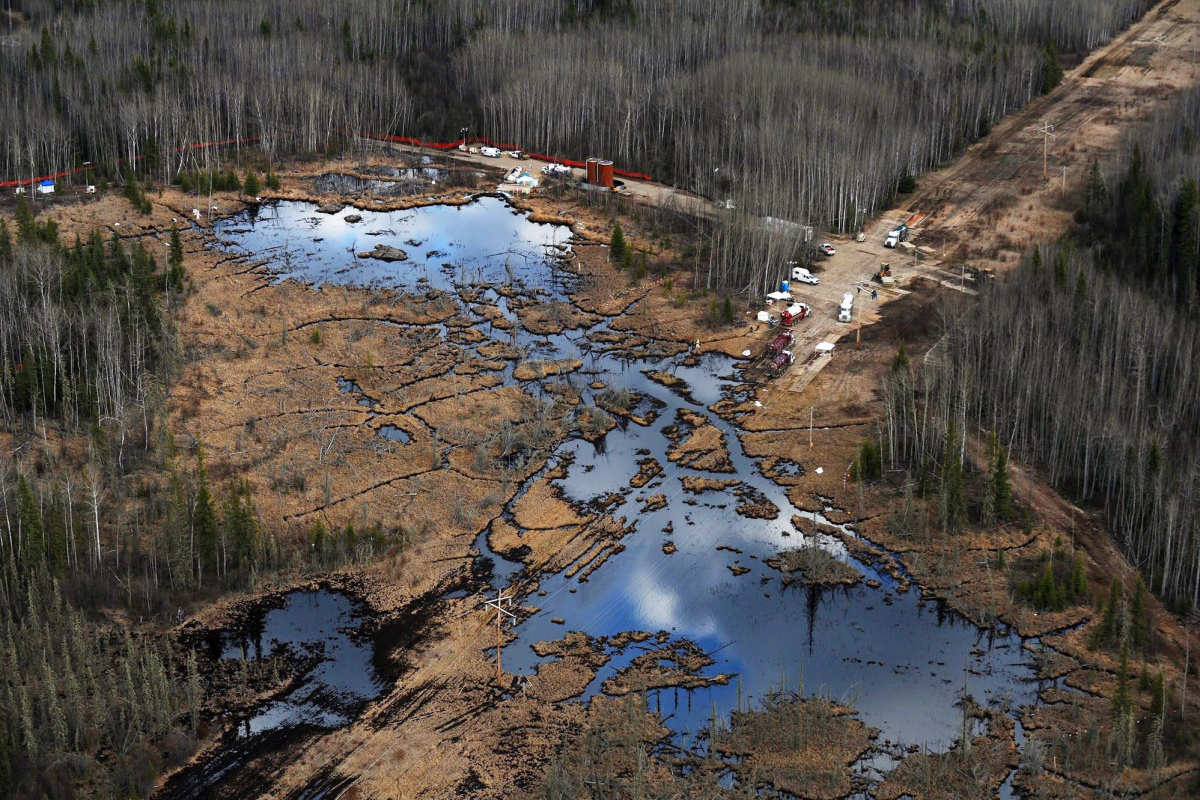
\includegraphics[width=100mm]{s3-pipeline-spill.png}
\centering
\caption{Pipeline spill northeast of Peace River, Alberta, on May 4th 2011. Source: Global News}
\label{fig:s3-pipeline-spill}
\end{figure}



A study conduced by Global News found that Alberta experienced 28,666 crude oil spills between 1975 and 2012.\footcite[][]{Young37Years}
This figure does not include spills from pipelines that cross provincial or national borders.
The study found that Alberta's Energy Resource and Conservation Board has been conducting a decreasing number of field inspections and finding more cases of ``high-risk noncompliance'': a figure that rose from 263 in 2010 to 437 in 2011.
Out of 362 drilling operations inspected, 41 were found to be ``high-risk noncompliant''.\footcite[][]{YoungPapernyRegulators}
According to the Energy Resources Conservation Board, Alberta experienced 700 crude oil and bitumen spills in 2012.\footcite[][]{YoungPapernyAnatomy}
The Canadian Natural Resources Ltd. Wolf Lake central treating facility has experienced 157 spills in the past 37 years.\footcite[][]{YoungPapernyAnatomy}
Imperial Oil Resources, Canadian Natural Resources Ltd., Husky Oil Operations Ltd., BP Canada Energy Company, the Encana Corporation, and Penn West Petroleum Ltd. have all experienced more than 1,000 oil spills since 1975: with total volumes ranging from 20,474 cubic metres to 79,505 cubic metres.\footcite[][]{YoungPapernyAnatomy}



In a 2010 study by a Royal Society of Canada Expert Panel, it was concluded that ``[r]eclamation [of land] is not keeping pace with the rate of land disturbance'' and that ``[c]urrent practices for obtaining financial security for reclamation leave Albertans vulnerable to major financial risks''.\footcite[][p. 5]{RoyalSocEnvHealth}
The study identifies that: ``increasing direct GHG emissions from growing bitumen production creates a major challenge for Canada to meet our international commitments for overall GHG emission reduction that current technology options do not resolve''.\footcite[][p. 5]{RoyalSocEnvHealth}
The study also finds major defects with environmental regulatory performance in Canada and Alberta.
It states that:
\begin{quote}
The environmental regulatory capacity of the Alberta and Canadian Governments does not appear to have kept pace with the rapid growth of the oil sands industry over the past decade. The EIA [Environmental Impact Assessment] process relied upon by decision-makers to determine whether proposed oil sands projects are in the public interest has serious deficiencies in relation to international best practice. Environmental data access for cumulative impact assessment needs to improve.\footcite[][p. 5]{RoyalSocEnvHealth}
\end{quote}
Each of these represents a substantial case of the business activities of fossil fuel companies frustrating the enforcement of domestic law and regulations intended to protect individuals against deprivation of health, safety, and basic freedoms.



A 2011 report from the Commissioner of the Environment and Sustainable Development found that the National Energy Board had been failing to follow up on identified deficiencies in the transport of dangerous products, that oversight of emergency procedures manuals was deficient, and that improvements were needed in implementing a risk-based monitoring approach.\footcite[][p. 21, 24, 26]{CESD2011Dec}
The report identifies that in cases where deficiencies were identified, they were not followed up in 93\% of cases.



The impact of climate change is being felt disproportionately in Canada's arctic.
This makes it a particular threat to the way of life of the Inuit.
Melting permafrost, the loss of summer sea ice, and impacts on marine mammal populations all threaten to substantially affect their way of life, culture, and economic subsistence.
Canadian Inuit activist and former International Chair for Inuit Circumpolar Council discusses these issues at length in her book \emph{The Right to be Cold}.\footcite[][]{RightToBeCold}



In addition, numerous pieces of Canadian environmental legislation explicitly recognize and seek to protect the right to a healthful environment.
The 1993 \emph{Ontario Environmental Bill of Rights} recognizes the ``inherent value of the natural environment'' and states that ``the people of Ontario have the right to a healthful environment'' and ``have as a common goal the protection, conservation and restoration of the natural environment for the benefit of present and future generations''.\footcite[][]{OntBillRights}
The purposes of the act are:
\begin{enumerate}
	\item to protect, conserve and, where reasonable, restore the integrity of the environment by the means provided in this Act;
	\item to provide sustainability of the environment by the means provided in this Act; and
	\item to protect the right to a healthful environment by the means provided in this Act.
\end{enumerate}
The above purposes include the following:
\begin{enumerate}
	\item The prevention, reduction and elimination of the use, generation and release of pollutants that are an unreasonable threat to the integrity of the environment.
	\item The protection and conservation of biological, ecological and genetic diversity.
	\item The protection and conservation of natural resources, including plant life, animal life and ecological systems.
	\item The encouragement of the wise management of our natural resources, including plant life, animal life and ecological systems.
	\item The identification, protection and conservation of ecologically sensitive areas or processes. (2). 
\end{enumerate}
Through numerous mechanisms described in this brief, the activities of fossil fuel companies undermine the integrity and sustainability of the environment, along with the right of the population of Ontario to a healthful environment.
GHG pollution poses an unreasonable threat to the integrity of the environment, while threatening biodiversity and the ability of Ontario to manage natural resources wisely and protect sensitive areas.



Environmental laws in Canada's provinces recognize and seek to protect the same right to a healthy environment.  
For example, the \emph{Yukon Environment Act} states that: ``The people of the Yukon have the right to a healthful natural environment''.\footcite[][p. 14]{YukonEnvAct}
Among its objectives, the act also seeks: ``to ensure the maintenance of essential ecological processes and the preservation of biological diversity'', ``to ensure comprehensive and integrated consideration of environmental and socioeconomic effects in public policy making in the Yukon'', and ``to fully use the knowledge and experience of Yukon residents in formulating public policy on the environment''.\footcite[][p. 13]{YukonEnvAct}
Because of the general failure to deal with climate change effectively in Canada, these objectives are currently being frustrated.
Similarly, the Northwest Territories \emph{Environmental Rights Act} recognizes that ``the people of the Northwest Territories have the right to a healthy environment and a right to protect the integrity, biological diversity and productivity of the ecosystems in the Northwest Territories'' and establishes the means by which individuals can act to protect the environment from harm.\footcite[][]{NWTEnvRightsAct}
By pursuing the extraction of fossil fuels, the companies in question undermine the right to a healthy environment that this act endeavours to protect. 
Finally, Quebec's \emph{Environmental Quality Act} states that: ``[e]very person has a right to a healthy environment and to its protection, and to the protection of the living species inhabiting it'' and that: ``A judge of the Superior Court may grant an injunction to prohibit any act or operation which interferes or might interfere with the exercise of [these] right[s]''.\footcite[][]{QuebecEQA}



In several instances, Canadian courts have recognized the seriousness of climate change in their decisions.\footcite[For a summary of the history of judicial interpretation of the powers of the federal and provincial governments concerning environmental protection, see Chapter 3 of: ][]{Harrison1996}

\begin{vcom}
Find as many examples as possible for the paragraph above. Make sure the final text here corresponds to the related question in the FAQ.
\end{vcom}


Over and above violations of specific pieces of legislation, climate change represents a massive example of `nuisance' as defined in Canadian tort law.
Under the common law in Canada ``a landowner's right to use and enjoy his property doesn't give him the right to engage in activities that interfere with the rights of neighbours to use and enjoy their own properties''.\footcite[][]{NuisancesInsider}
That is to say, the fact that fossil fuel companies own the land and mineral rights in the areas where they are operating does not mean they have the right to impose extreme weather, rising sea levels, and other well-understood climate change harms on other landowners across Canada.
This principle is also incorporated into the bylaws of many Canadian jurisdictions.
For instance, the town of Musgrave, Nova Scotia has a nuisance bylaw stating: ``No person shall cause, suffer or allow to be discharged or emitted from any fuel burning equipment, internal combustion engine, vehicle or outside open fire any smoke, dust, fly-ash, soot or fumes or other solid or gaseous product or combustion to an extent which is detrimental to the property of any other person''.\footcite[][]{NuisancesInsider}
Nuisances are also regulated under provincial and territorial law.



		\subsubsection{U.S. domestic law}



In a report prepared for the U.S. Congressional Research Service, Robert Meltz discusses many of the legal issues associated with climate change.\footcite[][]{ExistingLaw}
This includes questions about the power of various bodies to impose limits on GHG pollution.
It also includes issues of liability for harm caused by climate change, including through water shortages, sea level rise, and extreme precipitation.
While the answers to these questions are not clear in the United States, and barriers to litigation exist, it is conceivable that as the severity of climate change increases and the harms being imposed by GHG pollution become more evident, courts will show a greater willingness to recognize climate change as an issue where victims can seek recompense for damage and in which the unlimited appetite of polluters to make free use of the atmosphere may be curbed.



In 2007, the U.S. Supreme Court decided ``Massachusetts v. Environmental Protection Agency'' --- a suit brought by twelve states and several cities against the Environmental Protection Agency (EPA).\footcite[][]{MassVEPA}
The court held that the \emph{Clean Air Act} grants the EPA the authority to regulate tailpipe emissions of GHGs, and required the EPA to review its rationale for not regulating \ce{CO2} and other GHG emissions:
\begin{quote}
Under the clear terms of the \emph{Clean Air Act}, EPA can avoid taking further action only if it determines that greenhouse gases do not contribute to climate change or if it provides some reasonable explanation as to why it cannot or will not exercise its discretion to determine whether they do.\footcite[][p. 30]{MassVEPA}
\end{quote}
The court found that the failure of the EPA to regulate GHG emissions under the \emph{CAA} violated the law's ``clear statutory command''.\footcite[See: ][]{EPAhaspower}
In an April 17th 2009 decision, the EPA determined that six GHGs are indeed a danger to the environment and human health.\footcite[][]{GreenFigleaf}



Later in 2007, the U.S. Ninth Circuit Court of Appeals ruled on ``Center for Biological Diversity vs. National Highway Traffic Safety Administration''.\footcite[][]{9thcircuitHighway}
In this suit, the Center for Biological Diversity headed an alliance which included 11 states, two cities, and four environmental groups calling for rigorous analysis of greenhouse gas emissions in the \emph{National Environmental Policy Act} (NEPA) process. 
Specifically, this alliance challenged a rule broadcast by the National Highway Traffic Safety Administration (NHTSA) entitled: ``Average Fuel Economy Standards for Light Trucks, Model Years 2008-2011''.
This rule set corporate average fuel economy (CAFE) standards in accordance with the \emph{Energy Policy and Conservation Act} (EPCA), prior to the passage of a new energy bill.  
In this decision, the court overturned the government's lenient fuel economy standards for pick-up trucks and sport utility vehicles on the basis of a number of violations, including failure to adequately consider the greenhouse gas implications of the standards in the \emph{NEPA} analysis and ``failure to monetize the value of carbon emissions''.
The court found that the ``impact of greenhouse gas emissions on climate change is precisely the kind of cumulative impact analysis that \emph{NEPA} requires agencies to conduct''.
The Center for Climate and Energy solutions explains that ``[t]he court also discredited contrary precedent by stating more is now known about climate change'', holding that the 2007 ruling ``Massachusetts v. Environmental Protection Agency'' is ``more relevant than past cases where climate change science was allowed to be ignored''.\footcite[][]{NEPACases}
The \emph{New York Times} described the ruling as ``a major setback for both the auto industry and the White House at a time of growing public concern over the rising price of gasoline and the issue of climate change''.\footcite[][]{CourtRejectsTruckStandards}



Another example of a fossil fuel company frustrating U.S. domestic law can be found in the recent revelation that the oilfield services company Halliburton destroyed evidence related to the 2010 Gulf of Mexico oil spill.\footcite[][]{Halliburton2013}
Halliburton provided cementing services to BP, intended to help seal the well.
They advised BP that 21 `centralizer' devices should have been installed, to improve cementing, but BP chose to install only six.
After the disaster, ``Halliburton ordered workers to destroy computer simulations that showed little difference between using six and 21 centralizers''.\footcite[][]{Halliburton2013}
The disaster caused by the well blowout caused 11 deaths, along with substantial amounts of environmental and economic damage in the region.



		\subsubsection{Domestic law in other jurisdictions}
		
		
		
A limited recognition of the seriousness of climate change can be found in some legal decisions from the United Kingdom.
For instance, in 2008 jurors decided that damage caused by activists to the Kingsnorth power station in Kent was justifiable in light of the amount of environmental damage being done by the power plant.\footcite[][]{JuryDecides}
During the trial, the jurors heard testimony from NASA climatologist James Hansen.



When it added articles 71--74 to its constitution in 2008, Ecuador became the first nation to grant the environment the inalienable right to exist, persist, and be respected.
For instance, article 73 holds that: ``The State shall apply preventive and restrictive measures on activities that might lead to the extinction of species, the destruction of ecosystems and the permanent alteration of natural cycles''.\footcite[][]{EcuadorConstitution}
Following this example, Bolivia amended its constitution in 2011 with the Rights of Mother Earth Act (articles 56-60).\footcite[][p. 28--29]{BoliviaConstitution} \footcite[][]{BoliviaGives}



The domestic law of several other countries criminalizes ``ecocide'' --- a phenomenon defined by Polly Higgins as: ``The extensive damage to, destruction of or loss of ecosystem(s) of a given territory, whether by human agency or by other causes, to such an extent that peaceful enjoyment by the inhabitants of that territory has been or will be severely diminished''.\footcite[][]{EradicatingEcocide}
Article 342 of the \emph{Penal Code} of Vietnam concerns ``crimes against mankind'' and states that:
\begin{quote}
Those who, in peace time or war time, commit acts of annihilating en-mass population in an area, destroying the source of their livelihood, undermining the cultural and spiritual life of a country, upsetting the foundation of a society with a view to undermining such society, as well as other acts of genocide or acts of ecocide or destroying the natural environment, shall be sentenced to between ten years and twenty years of imprisonment, life imprisonment or capital punishment.\footcite[][]{VietnamPenalCode}
\end{quote}
Article 394 of the \emph{Criminal Code of the Republic of Armenia} similarly prohibits ecocide, as does the \emph{Criminal Code} of Belarus, the \emph{Criminal Code} of Moldova, the \emph{Criminal Code} of Ukraine, and the \emph{Criminal Code} of Georgia.\footcite[][]{ArmeniaCriminalCode} \footcite[][]{ICRConBelarusCC} \footcite[][]{MoldovaCriminal} \footcite[][]{UkraineCriminal} \footcite[][]{GeorgiaCriminal}



		\subsubsection{International law}



The activities of the fossil fuels companies in which the University of Toronto invests also frustrate international law.  
First, the \emph{Universal Declaration of Human Rights} states that ``Everyone has the right to life, liberty and security of person''.\footcite[][]{UniversalDeclarationOfHumanRights}
The right to life is a precondition to all other fundamental human rights.  
The activities of companies in the fossil fuels industry threaten the rights to life and security of the person through mechanisms including the increased frequency and severity of extreme weather, increased occurrence of infectious disease, and loss of  agricultural productivity.
In addition, the 1989 \emph{Hague Declaration on the Environment}, to which Canada is a signatory, makes the link between the right to life and the harmful effects of climate change explicit: ``The right to live is the right from which all other rights stem. Guaranteeing this right is the paramount duty of those in charge of all States throughout the world.  Today, the very conditions of life on our planet are threatened by the severe attacks to which the earth's atmosphere is subjected''.\footcite[][]{HagueDeclarationOnTheEnvironment}   
In signing onto this declaration, Canada recognized the reality of the threat to human life posed by climate change and pledged to take measures to address that threat.
The determination of fossil fuel companies to dig up and burn their entire reserves of coal, oil, and gas directly frustrates these international laws.
If fossil fuel companies are able to continue to operate under business-as-usual conditions and execute their business plans, the world will experience far more than 2˚C of climate change, with severe impacts on people everywhere.



Fossil fuel companies have repeatedly also frustrated the enforcement of the International Labour Organization's \emph{Indigenous and Tribal Peoples Convention, 1989}.\footcite[][]{ILOConv169}
This convention requires that indigenous populations be ``consulted on issues that affect them'' and that they be able to ``engage in free, prior and informed participation in policy and development processes that affect them''.
In many parts of the world, oil, gas, and coal extraction have taken place without such consultation, or even in the face of active and energetic opposition from indigenous groups.
The activities of Shell in the Niger Delta --- described more comprehensively in \nameref{sec:Shell} --- are an especially notable and egregious example.



The political influence of fossil fuel corporations in Canada has pushed the federal government to adopt obstructionist tactics at international climate change negotiations.
For example, Canada has repeatedly been `awarded' satirical `Fossil of the Year' award for obstructing negotiations at the Conferences of the Parties (COP) of the \emph{United Nations Framework Convention on Climate Change} (UNFCCC).\footcite[][]{DurbanFossil} \footcite[See also: ][]{SimpsonBlustering}
At the Copenhagen COP in 2009, a coalition of environmental groups declared Canada ``the absolute worst country at the talks''.\footcite[][]{CBCFossil}
Many countries questioned the appropriateness of Canada's frequent argument that it would not take more substantial action on the issue until ``all major emitters'' agreed to do likewise, despite the wide discrepancy between the historical and per-capita emissions of Canada and those of states like India.\footcite[][]{CanadaWontBudge}



\begin{vcom}
It would be good to have more evidence to substantiate the claim that the fossil fuel industry has undue influence with Canada's government: amount of contact between ministers and industry representatives, etc
\end{vcom}



The activities of fossil fuel companies are also at odds with the fundamental objective of the UNFCCC, which was ratified by Canada and which entered into force on March 21st 1994.
The UNFCCC affirms the intention of signatories to achieve ``stabilization of greenhouse gas concentrations in the atmosphere at a level that would prevent dangerous anthropogenic interference with the climate system''.\footcite[][p. 4]{UNFCCC}
Countries including Canada have since adopted a threshold of 2˚C of global temperature increase above pre-industrial levels as constituting `dangerous' climate change.
Canada's behaviour to date --- and the behaviour of fossil fuel companies --- has not been consistent with achieving this objective.
Achieving this objective requires that most of the reserves of fossil fuel companies be left unburned underground.
It also requires the abandonment of projects intended to extract unconventional reserves of fossil fuels, through activities including oil and gas drilling in the arctic, exploitation of the oil sands, and extraction of previously inaccessible oil and gas reserves through hydraulic fracturing.
Rather than curtailing such activities, the Government of Canada has worked intently to reduce the environmental oversight to which the oil sands are subjected, while aggressively pushing pipelines and other projects to increase the export capacity of the oil sands.\footcite[See: ][]{PeterKentTrail}



Despite ratifying the \emph{Kyoto Protocol} in 2002, the Government of Canada never developed an adequate plan to achieve the target it selected for itself: a reduction in GHG pollution to 6\% below 1990 levels by 2012.
In fact, Canadian emissions increased by 24.1\% between 1990 and 2008.\footcite[][p. 3]{UNFCCCCanada2010}
This frustrated the objectives of the \emph{UNFCCC} and \emph{Kyoto Protocol} both directly and indirectly.
It did so directly because Canada failed to reduce emissions as promised.
It also did so indirectly insofar as Canadian inaction was interpreted by countries around the world as evidence of Canada's lack of seriousness about confronting the problem of climate change, which could be used to justify inaction on the part of other countries. 



	\subsection{Why fossil fuels are like tobacco}
	\label{sec:LikeTobacco}



In 2007, the University of Toronto decided to divest from tobacco companies, after determining that the case to do so was consistent with university policies.
There are several important ways in which the tobacco precedent is relevant to fossil fuel divestment.



First, the scientific case demonstrating the harm caused by tobacco strengthened progressively over the span of decades.
Companies were initially willing to challenge these claims, but the weight of evidence eventually made their case untenable.
Similarly, the evidence demonstrating the seriousness of anthropogenic climate change has now progressed beyond the point where it can be considered a subject of ongoing academic inquiry and debate.



In the case of tobacco, the university considered it important that tobacco companies had undertaken a campaign to mislead the public and decision-makers about the dangerousness of their product.
The 2007 Report of the Advisory Board on Tobacco Investment cites the argument that:
\begin{quote}
The University should not be part owner of an industry that ``has deliberately set about to misinform the public'' and ``seeks to erode the very values that the University has vowed to protect''.\footcite[][p. 5]{TobaccoReport_2007}
\end{quote}
The efforts of the fossil fuel industry to mislead the public and elected officials are documented in Naomi Oreskes' \emph{Merchants Of Doubt} and James Hoggan's \emph{Climate Cover-Up}.\footcite[][]{MerchantsDoubt} \footcite[][]{ClimateCoverUp}
The conflicts between the actions of fossil fuel companies and the values of the university are documented throughout this brief, including the section on social injury.



Second, in both the cases of tobacco and fossil fuels the problem is the primary product being produced by the industry.
Just as it would be ineffective to use shareholder voice to try to convince a tobacco company to stop producing and selling tobacco, it is implausible that the university could use shareholder activism to convince fossil fuel companies to desist from activities that create and facilitate major greenhouse gas pollution.
When the university decided to divest from tobacco, it concluded that ``[t]he University of Toronto has neither the resources nor the jurisdiction to monitor the business practices of tobacco companies, or any other enterprises''.\footcite[][p. 7]{TobaccoReport_2007}
The same is true for fossil fuel companies; shareholder activism is not a credible strategy for influencing their decisions, and the university lacks the capability to effectively monitor them.



Third, both tobacco and fossil fuel consumption are distinct from other products that can be argued to cause social harm in that each item has ``no safe use''.\footcite[See: ][p. 9]{TobaccoReport_2007}
As acknowledged by University of Toronto President David Naylor in his letter regarding the university's decision to divest from tobacco shares, both anti-smoking advocates and major producers alike acknowledged tobacco's negative effects on human health.\footcite[][]{TStarSellOff}  
Similarly, environmentalists and scientists, along with spokespeople from the fossil fuel industry, have publicly conceded that the business of extracting and burning fossil fuels has multiple adverse effects on the ecological health of the planet as well as on global economic stability.\footcite[See, for example: ][p. 3--18]{OilIndustryVanDenHove}



Fourth, both investments in tobacco and fossil fuels challenge pre-existing policies that were developed and implemented in alignment with the university's core values. 
For instance, the case for tobacco divestment was logical given that an anti-smoking policy was already implemented on campus ``in recognition of the medical consensus on the health effects of smoking, and the University's place in the promotion of health''.\footcite[See: ][p. 9]{TobaccoReport_2007}
While no local, provincial or federal legislation banned the production of cigarettes or the activity of smoking on a universal scale, the absence of such regulations did not deter the university from divestment. 



The same logic can be applied to the case for divesting from fossil fuels. 
For instance, the university's Environmental Protection Policy, developed in 2010, reflects the university's commitment ``to being a positive and creative force in the protection and enhancement of the local and global environment''.\footcite[][]{UTEnvProtectionPolicy}
Divestment from fossil fuels is a legitimate action in recognition of the governmental and scientific consensus on the detrimental effects of fossil fuel extraction and consumption, and in acknowledgment of the university's own position on promoting environmental health as stipulated in its Environmental Protection Policy as well in its academic programming.\footnote{See: \nameref{UTTakenSides}}



In the absence of legislation banning the extraction or burning of fossil fuels, recognition of the adverse effects of these activities, legitimated through the enactment of the Environmental Protection Policy and other university initiatives, constitutes legitimate basis for divestment based on the precedent of the tobacco case.  



Furthermore, the ability and desire to divest in the absence of official legislation that can be cited to validate claims of ``social injury'' is possible and has precedent in the events leading up to the university's decision to divest from companies operating in apartheid South Africa. 
For instance, in response to growing social pressure calling for an end to apartheid and to international complicity in the system, the Canadian government passed Bill 9, \emph{An Act Permitting Trustees and other Persons to dispose of South African Investments}.
This piece of legislation was tabled first on November 5th 1987 and enacted in the Legislature of Ontario on December 15th, 1988. 
However, the Governing Council at the university voted to divest from stocks held in South African companies on January 21st 1988, almost a full year before Bill 9 was passed. 
This progressive action on the part of the university represents a forward-thinking response to the trajectory of social sentiment regarding the issue of apartheid, which was growing rapidly and was manifesting itself in policy changes and legislation such as Bill 9. 



While no such Canadian legislation currently exists with regards to the extraction and burning of fossil fuels which are the direct causes of climate change, we propose that the university give the same weight to the strengthening consensus amongst governments, scientific organizations, and financial institutions that are increasingly recognizing the risks of climate change not only to human health and ecosystems but to global economic stability and, by direct implication, to the maintenance of sound investment policies.



The tobacco precedent is also relevant to the question of whether divestment from Shell is likely to harm the university financially. For more information, see: \nameref{sec:ShellNotFinancialHurt}



% END SECTION 3 - MIE

% END SECTION 3 - TAMARA AND MIE



% BEGIN SECTION 4 - STUART
% FIDUCIARY DUTIES

% BEGIN SECTION 4 - STUART
% Last updated by Milan Ilnyckyj 2013-07-30



		\singlespacing
		\section {Divestment is compatible with the university's fiduciary duties}
		\label{sec:Fiduciary}
		\doublespacing
		


% Has incorporated comments from Alena Prazak



		\subsection {From the U of T divestment policy}
		
		
		
\begin{itquote}    
(i) prudent investment. The University has a fiduciary duty to manage investments responsibly to maximize return on its investments within a policy risk tolerance as approved by Business Board from time to time.

...

The committee will consider the following guidelines in considering the appropriate response to any request:
\begin{itemize}
  \item the extent and significance of the University's investment in a particular entity. Determination of whether investments are considered significant will depend on the committee's judgment of the relative magnitude of the University's holdings both as a fraction of all University investments and in relation to the market capitalization of the entity under review.
  \item the degree to which the entity itself is involved in the undesirable activity.
\end{itemize}
Normally, activity is considered significant if more than ten percent of the entity's revenues are derived from the undesirable activity.
\end{itquote}



	\subsection{Fossil fuel divestment is financially responsible}

	

Any fiduciary has two main factors to consider in investments: risk and return.
Fossil fuel divestment offers considerable potential to mitigate important risks, while creating only negligible new ones.
In addition, the historical returns of a portfolio that excludes fossil fuel stocks are comparable to those with no such exclusion, and there are good reasons to believe that the future returns of non-fossil-fuel investments will be competitive.
This section will consider both the financial case for divestment and questions about the practicality of divesting from a financial perspective, including in terms of the fiduciary duties borne by the University of Toronto.



In advice provided to the United Nations Environment Programme Finance Initiative, Freshfields Bruchhaus Deringer considered the relationship between fiduciary duty and environmental, social and governance (ESG) issues within common law jurisdictions.
They explain that: ``[t]he modern prudent investor rule, which incorporates both a duty of care and a duty of loyalty, emphasises modern portfolio theory and provides that: ... there is no duty to `maximise' the return of individual investments, but instead a duty to implement an overall investment strategy that is rational and appropriate to the fund''.\footcite[][p. 6]{UNEPFinanceInit}
They go on to explain that: ``[t]here is accordingly no reason why investment strategies should not include investments with positive ESG characteristics. The important limiting requirement is that imposed by the duty of loyalty: all investment decisions must be motivated by the interests of the fund's beneficiaries and / or the purposes of the fund.''\footcite[][p. 6]{UNEPFinanceInit}
Discussing Canada specifically, they explain: ``the power of investment is undertaken in a prudent manner when adequate processes (including completion of studies of the nature and quality of a proposed investment in light of the plan's total assets and obligations) have been followed and salient information (including expert opinions) has been considered''.\footcite[][p. 51]{UNEPFinanceInit}
The report lists a number of major Canadian institutional investors that have incorporated ESG issues into their processes, including the Ontario Municipal Employees Retirement System, the Ontario Teachers' Pension Plan Board, and the Canada Pension Plan Investment Board.\footcite[][p. 52]{UNEPFinanceInit}
In the same report, they claim: ``Climate change is an obvious example of an environmental consideration that is recognised as affecting value.''\footcite[][p. 11]{UNEPFinanceInit}
As this brief explains in detail, the beneficiaries and purposes of the University of Toronto's investments will be well-served by fossil fuel divestment.
Such divestment will not be financially harmful, will help the university reduce exposure to important risks, and will be in keeping with the values and reputation of the institution.



The Freshfields advice accords with advice that U of T itself sought, in the case of tobacco divestment in 2007.
Mr. Timothy Youdan of Davies Ward Phillips \& Vineberg was hired to produce a legal opinion on the University's investment policy with respect to a proposed prohibition on investment in the tobacco 
industry.
Mr. Youdan found that: ``the position taken in England by the Pension Law Review Committee 
is applicable in Ontario and applicable to trustees of a charity as well as pension trustees''.
He found further that this allows: ``pension trustees to properly exclude investments for nonfinancial reasons if doing so will not have a detrimental effect on the financial performance of the fund''.\footcite[][p. 6]{TobaccoReport_2007}



The International Energy Agency argues that: ``the deployment of a low-carbon energy system... delivers wide benefits by enhancing energy security, environmental protection and economic growth'', that: ``a low-carbon energy system increases energy security, particularly for energy importing countries, through reduced energy dependence and greater diversity of energy sources and technologies'', and that: ``the pathway to [stabilizing global temperatures at less than 2˚C above pre-industrial levels] is not just environmentally necessary but economically sound''.\footcite[][]{IEAOnTwoDegrees}
They argue that the net benefit of decarbonization amounts to US\$61 trillion if not discounted and US\$5 trillion if using a 10\% discount rate.
Furthermore, they argue that: ``low-carbon technologies often also reduce local air pollution, providing other environmental benefits and improve quality of life''.



\subsection {There is no evidence of a divestment penalty for investors}
\label{NoDivestPenalty}



Several studies have attempted to quantify the financial consequences of taking environmental factors into account in the investment management process.
In aggregate, these studies found no significant impact on investment risk in predictive models, nor a performance penalty in tests using historical data.
\begin{description}
  \item[Historical] The UN Environment Program Finance Initiative's analysis of twenty academic studies on the effect of incorporating Environmental, Social and Governance factors in the investment management process found there to be no evidence of a resulting performance penalty. The two reviewed studies that focused specifically on environmental factors found a positive relationship between consideration of those factors and performance.\footcite{UNEPFI2007}
  \item[Risk Based Assessment] The Aperio Group found that divesting from the ``Filthy Fifteen'' ``increases absolute portfolio risk by only 0.0006\%, or about a half of one one-thousandth of a percent.'' Even divesting from the entire Fossil Fuel sector only results in a 0.0034\% return penalty.\footnote{For the purposes of this study, the ``Filthy Fifteen'' was defined as the group of 15 U.S. companies judged by As You Sow and the Responsible Endowment Coalition to be the most harmful based on the amount of coal mined and coal burned along with other metrics.''} In other words, the portfolio does become riskier, but by such a trivial amount that the impact is statistically insignificant.\footcite{Aperio2013}
  \item[Forward Looking] Carbon Tracker and Standard \& Poors together conducted a study on the implications of carbon constraints for credit ratings of the oil and gas sector. Their scenario assumes reducing demand for \ce{CO2}-intensive fuels, in line with the internationally recognized limit of a 2˚C rise in global temperatures, and is ``not materially different from the current price deck assumptions.'' The study concludes with the statement:
\begin{quote} 
[A]s the price declines persist in our stress scenario of weaker oil demand, meaningful pressure could build on ratings. First to be affected would be the relatively focused, higher cost producers, and then the more diversified integrated players. In both cases, according to our study, the causes would be a decline in operating cash flows, weakening free cash flow and credit measures, along with less certain returns on investment and less robust reserve replacement.\footcite{SandPConstrained}
\end{quote}
  \item[Meta Analysis] It is frequently assumed that excluding the fossil-fuel sector from a portfolio will inevitably lead to a reduced performance, due to the reduction in potential investment opportunities.
  However, empirical research has repeatedly shown this assumption is fallacious.
  Deutsche Bank and Mercer have conducted major meta-studies that discovered the vast majority of academic studies of ESG investment performance found the incorporation of ESG factors into portfolio management to be either neutral or positive.\footcite{DeutscheBankSI} \footcite{MercerRI}
  \item[Case Study] Portfolio 21, based in Portland, Oregon, created one of the first sustainability-themed global equity mutual funds, known as Portfolio 21 Global Equity Fund (PORTX). The institutional share class has outperformed its benchmark by 105 basis points annualized over the past five years and by 93 basis points annualized over the last decade. Portfolio 21 has therefore demonstrated for more than a decade that a global investment strategy that avoids fossil fuels --- and many other unsustainable industries --- need not come at the cost of financial performance or increased portfolio risk.\footcite{FossilFreeInvesting}
\end{description}
Canadian socially-responsible investment funds like the NEI Ethical Canadian Dividend A fund --- which tries to balance social concerns with returns --- have outperformed the S\&P / TSX total return in 2013.\footcite[][]{HoldTheirOwn}



In July 2013, Impax Asset Management published a study examining the last seven years worth of data on international equity markets.
They compared a portfolio consisting of the MSCI World Index with another in which fossil fuel stocks were excluded and determined:
\begin{quote}
Excluding the fossil energy stocks from the MSCI World Index over the last seven years (to the end of April 2013) would have had a small positive impact on returns (0.5\% annually) and only a modest increase in tracking error of 1.6\% a year. For the five years to the end of April 2013, which excludes the dramatic run up in energy prices ahead of the 2008 financial crash, excluding the fossil energy sector would have improved returns by almost 0.5 percentage points annually, to 2.3\% a year from 1.8\%. Again, tracking error is low at 1.6\%.\footcite[][p. 5]{ImpaxBeyondFF} \footcite[See also: ][]{ImpaxEnergyCollective}
\end{quote}
These conclusions are echoed in recent analysis from MCSI ESG Research:
\begin{quote}
Over the period from January 2008 through March 2013, the market capitalization of the 247 fossil fuel reserve-owning companies described above ranged from approximately 7 percent to 8 percent of the MSCI ACWI IMI. Hence, excluding these stocks left between 93 percent and 94 percent of the MSCI ACWI IMI intact over the time series in terms of market capitalization. This meant that for each 10 percent active return differential in the carbon reserve stocks relative to the MSCI ACWI IMI, the effect of removing these stocks from the index ranged from 0.7 percent to 0.8 percent (70 to 80 basis points) in changes to active returns. Nearly all of this effect was due to industry factors, as opposed to country exposure and other style factors. As shown in the chart below, the performance of the MSCI ACWI IMI excluding the carbon reserve stocks closely tracked the MSCI ACWI IMI over the time series. Slight underperformance of the ``ex Carbon list'' appeared near the beginning of the time series, and slight outperformance of the ``ex Carbon list'' emerged toward the end of the time series. The active return differential over the entire time series was 1.2 percent (120 basis points) in favor of the ``ex Carbon list'' relative to the full MSCI ACWI IMI. The tracking error relative to full index was 1.9 percent (190 bps).\footcite[][p. 5]{MCSIFFP}
\end{quote}
There is reason to believe, therefore, that divestment would involve only a limited risk of foregoing improved ratings and investment returns.
Indeed, divestment could actually benefit the portfolio, in that it would remove risk of being invested in companies whose ratings only appear likely to decline in the long term.



	\subsection {Market capitalization and value at risk}



In a report for the Canadian Centre for Policy Alternatives, Marc Lee and Brock Ellis explain that: ``Canada is experiencing a carbon bubble that must be strategically deflated in the move to a clean energy economy''.\footcite[][p.5]{CanadaCarbonLiabilities}
Even with a high estimate of how much of the world's total carbon budget Canada can use up, they conclude that: ``78\% of Canada’s proven reserves, and 89\% of proven-plus- probable reserves... need to remain underground''.\footcite[][p.6]{CanadaCarbonLiabilities}
In short, the business plans and stock market valuations of fossil fuel companies are based on the unjustified assumption that they can continue to use the global atmosphere as a free dumping ground for greenhouse gas pollution.
As the injury caused by climate change has more obvious, governments have become increasingly willing to regulate fossil fuel use.
This progression can be expected to continue in the future, eventually compelling fossil fuel companies to leave significant reserves unburned.\footcite[See, for instance: ][]{ThreatenGrowth}
If the damage from fossil fuel burning amounts to \$50 per tonne (the low end of Lee and Ellis' estimate) then the damage that burning all Canadian fossil fuels would do amounts to \$844 billion, equivalent to two-and-a-half times the market capitalization and nearly twice the total assets of Canadian fossil fuel companies.
Based on a high damage estimate of \$200 per tonne, burning Canada's fossil fuel reserves would cause \$5.7 trillion in damage --- a figure 17 times larger than the market capitalization of these 144 firms and 13 times larger than their assets.
The analysis from Lee, Ellis, and others makes two things clear: burning fossil fuels causes very substantial amounts of social injury, and the prospect of strengthened regulations on greenhouse gas pollution threatens the profitability and stockmarket value of fossil fuel companies.



A recent article in the \emph{National Post} describes the `carbon bubble' and the risks it poses for investors: ``energy sector valuations ignore the world's climate change target and could be decimated if the international community puts its money where its mouth is and collectively moves to protect Mother Earth by attacking demand for oil, coal and gas''.\footcite[][]{OilGiantsMajorPain} \footcite[See also: ][]{TimelyIssue}
It goes on to explain: ``if the international community gets serious about its stated [2˚C] temperature goal, about two-thirds of existing energy sector reserves, which currently support about US\$4 trillion in share value and back more than US\$1 trillion in debt, are actually superfluous to the world's needs''.
The Climate Commission established by the Australian government echoes these findings.\footcite[][]{CriticalDecade2013}
Simon McKeon, the executive chairman of the commission, argues that: ``[a]nyone who believes they have literally hundreds of millions tonnes of first rate high emitting \ce{CO2} coal can no longer blindly believe there will be a strong market for that in 20, 30 years'' and that ``the best of resource investors are absolutely on to this''.\footcite[][]{CoalWillBeLeft}



	\subsubsection {Stated policy objectives are incompatible with the current valuation of fossil fuel reserves}



Fossil fuels may provide a hedge against other asset classes, but only in scenarios where unconstrained emissions lead to accelerated and possibly catastrophic warming. 
The international community is in broad agreement that this must not happen.



	\subsubsection {Regulatory risk is not adequately priced} 



As one scenario for the \emph{World Energy Outlook} in 2012, the International Energy Agency assumes international cooperation to keep \ce{CO2} under 450ppm, which in their model constrains the likelihood of warming greater than 2°C to 55\%. 
This is in contrast to their baseline New Policies Scenario, which assumes modest reductions in the rate of emissions increase compared to the third scenario, Current Policies. 
Evaluating the effect of this scenario on the price of fossil fuels, they estimate:
\begin{quote}
Compared with the New Policies Scenario, the global oil price in the 450 Scenario in 2035 is \$25 per barrel lower and the coal price almost 40\% lower. The price for natural gas falls by 23\% in Europe and 4\% in North America.\footcite[][p. 257]{IEA2012}
\end{quote}
In a report for the Australian National University and the Investor Group on Climate Change, Dr. Michael H. Smith concluded that: ``Climate change is forecast to dramatically increase the exposure of oil and gas companies to climate, energy and carbon price risks''.\footcite[][p. 14]{RisksForInvestors}



For any scenario where emissions are constrained to keep warming under 2°C, market assumptions regarding the profitability of fossil fuel extraction are necessarily optimistic. 
Marginal projects will become unprofitable and returns to investors for even the most profitable projects will decline. 
Indeed, the study conducted by Standard \& Poors even indicates near-term threats to the stability of investing in some fossil fuel companies: ``Under our stressed scenario, the ratings on companies with high development and production costs, including those focused on unconventional resources, could see rating pressure build \emph{within one or two years}, especially if the companies are relatively undiversified'' (emphasis ours).\footcite{SandPConstrained}
The study continues: ``We see a deterioration in credit measures for these smaller oil companies over 2014--2015, to a degree that could potentially lead to negative outlook revisions and downgrades over 2014--2017... this could result in an earlier deterioration in our business risk profile assessments''.
Furthermore, even ``the financial risk profiles of the oil majors would weaken modestly over the next five years''.
It is also worth noting that the study claims: ``the core business model [of fossil fuel companies] could come into question,'' and that ``this could potentially result in \emph{a downgrade of more than one notch} if we were to place less reliance on undeveloped or probable reserves than at present'' (emphasis ours).



The possibility of significant new climate regulations in the years ahead is not idle.
The Obama administration is expected to move forward with emissions limits on existing power plants.\footcite[][]{ReadyingLimits} \footcite[][]{ObamaJune2013}
In anticipation of his June 25th 2013 climate speech, in which he was expected to announce restrictions on \ce{CO2} emissions from existing coal plants, the stock price of major coal companies fell significantly: shares in Consol Energy fell 7.2\%, those in Cliffs Natural Resources fell 7.6\%, Peabody Energy's share price fell 7.2\%, and those in Alpha Natural Resources fell 8\%.\footcite[][]{CoalSharesPlunge} \footnote{All four companies are included in \nameref{sec:200Companies}}
The speech saw President Obama pledge to regulate \ce{CO2} emissions from existing power plants, promote the deployment of renewable energy, modernize the electrical grid, and further increase fuel economy standards for vehicles.
The fall in the stock value of coal companies deepened after the details of the new Obama plan were announced.\footcite[][]{CCPlanPoundsCoal}
The Government of China may also be considering imposing a carbon tax.\footcite[][]{ChinaTaxingCarbon}
Tightened regulations could pose a major risk for the value of fossil fuel companies.
A study by HSBC concluded that: ``Oil and gas majors, including, BP, Shell and Statoil, could face a loss in market value of up to 60 percent should the international community stick to its agreed emission reduction targets''.\footcite[][]{EconomicCase}



	\subsubsection {There is a strong potential for malinvestment in capital-intensive, long-term projects}



The IEA's 2012 World Energy Outlook concluded that, ``more than two-thirds of current proven fossil-fuel reserves cannot be commercialized in a 2˚C world before 2050.'' \footcite{IEA2012}
The Standard \& Poors Carbon Tracker Initiative study raises concerns concerning the fossil fuel sector: ``This illustrates to us the apparent divergence between the assets owned by coal, oil, and gas companies and the direction of negotiations at UNFCCC conferences.'' \footcite{SandPConstrained}
The study concludes that up to \$6 trillion could be wasted in fossil fuel investments that become unviable because of tightened climate change policies globally.\footcite[][]{SixTrillionBubble}
As explained by the National Round Table on the Environment and the Economy (NRTEE):
\begin{quote}
Every year of delay in sending strong, economy-wide policy signals represents a wasted opportunity to take advantage of natural cycles of infrastructure and equipment renewal, making it more difficult and expensive to meet emissions reduction targets. Our analysis shows that waiting until 2020 to implement climate policy aimed at cutting emissions by 65\% from 2005 levels by 2050 implies close to \$87 billion in refurbishments, retrofits and premature retirement of assets.\footcite[][p. 19]{FramingFuture}
\end{quote}
Another study found that up to 75 gigawatts of coal-fired electricity capacity will need to be retired by 2030 because of tightened environmental regulations.\footcite[][p. 10]{RisksInCoal}
Investment in \ce{CO2}-emissions-enabling infrastructure is contrary to the international community's consensus about the direction of the future.

% Milan had proofread up to here, 1:50am 2013-06-25

The persistently high price of fuels on the world market in recent years has lead to unprecedented investment on the part of the fossil fuel industry in projects that were previously deemed too marginal to profitably develop. 
Development of unconventional hydrocarbon reserves such as tar sands, oil shale, offshore drilling in extremely deep water and the arctic, hydraulic fracturing and mountaintop removal coal mining entails extremely high capital investment. 
Scenarios in which carbon emissions are restricted sufficiently to keep global temperatures from rising more than 2°C would likely cripple the return on much of this investment.



In anticipating restrictions on carbon emissions, the fossil fuel industry has been pinning its hopes on the development of effective methods of carbon capture and sequestration (CCS). 
Despite tremendous investment in CCS technology on the part of both the private and public sectors, economically feasible sequestration of emissions at scales needed to mitigate climate change remains elusive.\footnote{For more information on CCS, see: \nameref{CCSSaves}}
There are currently no commercial scale CCS projects in operation on the planet, and in 2008 Cambridge Energy Research Associates (CERA) predicted that it would be another two decades before CCS saw large-scale deployment. \footcite{CERACrossing}
According to the Carbon Tracker Initiative, even if CCS is deployed in line with an idealised scenario by 2050, this would only extend fossil fuel carbon budgets by 12-14\%, or just 4\% of total global reserves.\footcite{CTI2013}
It must be remembered that at the current rate of global carbon emissions, the entire budget of carbon emissions would be spent by the late 2020s, several years before large-scale CCS can be expected to come online.\footcite{CTI2012}



CCS has many other problems associated with it. For example, CCS would use extra energy, potentially as much as 40\% of the power generated by a power station. \footcite{GPCCS}
This reduces the efficiency of the power plant, both increasing financial costs and increasing the amount of fuel needed per energy output, which in turn contributes to the problems associated with fossil fuel extraction.
Indeed, the increased cost of the energy provided by CCS-enabled power stations would likely be higher than the cost of energy from renewable sources, and so would almost certainly never be implemented. \footcite{SmartPlanetCCS}
Storing carbon underground is risky --- safe and permanent storage of \ce{CO2} cannot be guaranteed, and even very low leakage rates could undermine any climate mitigation efforts. \footcite{GPCCS}
Finally, money spent on CCS will divert investments away from sustainable solutions to climate change, which the world will need to transfer to eventually, whether or not it burns all the available (non-renewable) fossil fuels.
Therefore, pinning our hopes on a non-existent technology, that is likely to both be more expensive and problematic than other energy sources, is a false hope.



	\subsubsection {Fossil fuel reserves as stranded assets} 



Given the degree to which proven reserves of carbon exceed allowable emissions for sub-2°C warming, companies with fossil fuel reserves as their largest assets may be substantially overvalued under current market conditions. 
Stranded assets in the form of unburnable reserves and large liabilities incurred to develop those reserves combine to create a risk not only to equity, but to bondholders as well.
The Carbon Tracker Initiative reports that in 2012 the Fossil Fuel sector spent \$674 billion prospecting for new sources of carbon, sources which cannot be exploited if the 2°C target is to be met. \footcite{CTI2013}


As the Carbon Tracker Initiative's 2012 report made clear, fossil fuel companies have significantly more exploitable sources of carbon available than is safe to burn. \footcite{CTI2012}
Therefore, when considering ``What A Carbon-Constrained Future Could Mean For Oil Companies' Creditworthiness,'' Standard \& Poors decided that, ``instead of considering issues of peak oil in terms of supply, this introduces a concept of peak oil demand.'' \footcite{SandPConstrained}
Whether they took the form of tightened efficiency requirements, the establishment of a cap-and-trade scheme, or the promulgation of a carbon tax, enhanced climate regulations would generally have the objective of reducing fossil fuel demand.
A reduction in oil, gas, and coal demand would have serious consequences for the fossil-fuel industry, particularly in Canada.



For example, MIT conducted a study that explored the effects \ce{CO2} emissions reduction policies would likely have on Canada's bitumen industry.
The study reaches the conclusion that, ``with \ce{CO2} emissions caps implemented worldwide, the Canadian bitumen production becomes essentially non-viable even with CCS technology, at least through our 2050 horizon.'' \footcite{MITConstraints}



As any investment manager knows, past performance does not guarantee future results, and it is becoming increasingly common for analysts and investors to discuss the prospect that the historical outperformance of fossil-fuel companies may be similar to the tech boom of the 1990s and the housing bubble of recent years.
However, the so-called ``carbon bubble'' potentially poses a much greater risk than either of these previous bubbles.
``Conservative estimates for the financial worth of the unburnable carbon reserves have ranged from \$20 trillion to \$27 trillion, so any associated write-down of fossil-fuel company valuations could very easily dwarf the recent \$2 trillion housing meltdown—by a full order of magnitude.'' \footcite[][p. 3]{FossilFreeInvesting}
According to John Fullerton, founder and president of the Capital Institute, this multi-trillion ``externality'' presents civilization with a ``Big Choice'': ``either we must absorb a \$20tn write-off into our already stressed global economy over the next decade, or we will implicitly accept civilization-transforming climate change''.\footcite{BigChoice}



\subsubsection {Volatility of investor sentiment}



Current market capitalization of the fossil fuel industry rests in part on the assumption that the global investor class will continue to see the sector as a reliable investment even as damage from climate change becomes apparent. 
This assumption has been increasingly challenged from both outside and within the financial industry. 
Traditionally conservative-minded publications such as \emph{The Economist}, \footcite{EconomistUnburnable} \emph{Business Week} \footcite{BusinessWeekOvervalued} and the \emph{Financial Times} \footcite{FTOvervalued} have published articles suggesting the fossil fuel sector is overvalued. 
In recent months, other voices within the financial industry such as investor groups and hedge fund managers have been increasingly sounding the alarm over the ``Carbon Bubble''. \footcite{JeremyGrantham} 
The Guardian recently reported
\begin{quote}
The message to all the players across the financial chain, from ratings agencies through accountants, to actuaries, investment advisors and all the rest, is also obvious. If the regulators won't do their job, do it for them. \emph{Jump, before you are pushed} (emphasis ours). \footcite{Guardian6Trillion}
\end{quote}
The afore-mentioned Standard \& Poors study, which saw a declining trend on both the short-term and long-term outlook for fossil fuel companies (both mid-size and large), reached its conclusion without ``explicitly [factoring in] any mitigating measures such as ... material cuts in near-term capital investment.'' \footcite{SandPConstrained}
However, there is already a significant, international fossil-fuel divestment movement that could result in such material cuts: over 300 colleges and universities and over 100 cities and states currently have divestment campaigns, along with several religious institutions.\footnote{For detailed information on the status of ongoing divestment campaigns, see: \nameref{PeerSchools}}




	\subsection {Fossil fuels represent a risk to the university's other investments}



Institutional investors, and universities in particular, are often expected to plan financially on a timescale far longer than average. 
On timescales of 50 years or more, the consequences of unconstrained emissions are very likely to overshadow all other financial considerations.
According to a 2012 report by DARA, climate change is already costing the world more than \$1.2 trillion, wiping 1.6\% annually from global GDP.
By 2030, the researchers estimate, the cost of climate change and air pollution combined will rise to 3.2\% of global GDP, with the world's least developed countries forecast to bear the brunt, suffering losses of up to 11\% of their GDP. \footcite{DARACVM}
Going further into the future is increasingly hard to predict, with estimates varying widely: the Stern Review estimates losses of between 5\%-20\%, \footcite{Stern2007} and a United Nations report asserts that climate change could cost Latin American and Carribean countries 137\% of GDP by 2100. \footcite{CCLatinAmerica}
However, regardless of the variations of predictions, the trend is clear: the more the climate changes, the greater the reductions to GDP.
As the Stern Review explains, ``[t]he benefits of strong, early action on climate change outweigh the costs''.\footcite[][Executive summary at: \url{http://www.hm-treasury.gov.uk/d/Executive_Summary.pdf}]{Stern2007}
Therefore, mitigating climate change can be expected to result in a relatively higher GDP, and to result in greater returns on the university's investments over the long term.\footcite[See also: ][]{EconomicCase}



In 2012, the National Round Table on the Environment and the Economy studied the risks posed to business by climate change.
They identified many categories of associated risk, including fire and property damage, storms and other natural perils, business interruption, disease and disability, and liability claims.\footcite[][p. 3]{ManagingBusinessRisks}
The report concludes that: ``some industries will be impacted significantly and permanently''.\footcite[][p. 2]{ManagingBusinessRisks} \footcite[See also: ][]{LeveragingInvestmentsCScience}
They project that climate change will cost Canada roughly \$5 billion per year by 2020, rising to between \$21 billion and \$43 billion per year by mid-century.\footcite[][p. 2]{ManagingBusinessRisks}
In ``Facing the Elements: Building Business Resilience in a Changing Climate'', the NRTEE identifies the oil and gas sector, mining, agribusiness, retail and distribution, hydroelectricity, technology and communications, and financial services as industries at risk of being negatively impacted by climate change.\footcite[][p. 9--10]{FacingTheElements}




	\subsection {Attractive substitutes exist for divested equities}



There are many attractive alternatives that could form substantial portions of the university's portfolio.
The renewable energy sector has enormous growth potential and is starting to match even conventional fossil-fuel energy prices (let alone unconventional energy prices).
According to NRTEE: ``Understanding the implications of the global low-carbon transition for Canada and making choices that maximize the opportunities and minimize the risks are critical to Canada's long-term prosperity''.\footcite[][p. 15]{FramingFuture}
In particular, they argue that the ``public and private sectors need to mobilize investment in low-carbon infrastructure and technology''.\footcite[][p. 17]{FramingFuture}
Unsubsidised renewable energy is now cheaper than electricity from new-build coal- and gas-fired power stations in Australia, according to new analysis from research firm Bloomberg New Energy Finance. \footcite{BlombergAussieWind}
Solar power is predicted to be cheaper than fossil fuel power in the USA as soon as 2015. \footcite{GlobalDataSolar}
In March 2013, 100\% of the new energy on the U.S. grid was solar power. \footcite{SmartPlanetSolar100}



There are three broad-based mutual funds that are completely fossil free: Green Century Balanced Fund (GCBLX), Portfolio 21 Global Equity Mutual Fund (PORTX), and Shelton Green Alpha Fund (NEXTX). \footcite{GFFMyMoney}
The GCBLX is solidly in the middle of its grouping regarding overall rating, returns and risk of the category, \footcite{GCBLX} and as mentioned earlier, the PORTX has actually out-performed its peers. \footcite{PORTX}
The Shelton Green Alpha Fund only started recently, and hasn't yet received a rating. \footcite{NEXTX}



There is a body of credible evidence demonstrating that environmental, social and governance (ESG) considerations often have a role to play in the proper analysis of investment \emph{value}. 
As such they cannot be ignored, because doing so may result in investments being given an inappropriate value.
A UNEP Finance Initiative report points out, ``many people wonder what good an extra percent or three of patrimony are worth if the society in which they are to enjoy retirement and in which their descendants will live deteriorates.'' \footcite{UNEPFinanceInit}
The report notes that, in Canada, there is an increasing frequency of debate regarding ESG issues, and that there is ``considerable and persistent support'' for increased consideration of ESG investment strategies.



\subsection {Pensions and climate change}



Pensions are intended to allow the pensioner to enjoy a satisfactory, even comfortable, retirement.
However, the more the climate changes, the lower the retirees' quality of life will be.
A study conducted by the World Bank makes it clear that a 4˚C hotter world will be a much more hostile world than one in which there has only been a 2˚C rise, with 6˚C or greater rises being more hostile still. \footcite{WorldBank4C}
The previous sections of this brief demonstrate that even a 2˚C rise will result in a greater frequency of natural disasters than the relative climate stability of the development of human civilisation thus far.
Indeed, the world's top scientists have calculated that a concentration of \ce{CO2} in the atmosphere that is higher than 350ppm is not compatible with the planet ``on which civilization developed and to which life is adapted.'' \footcite{TargetAtmosphere}
The relationship between pension obligations and climate change has already been acknowledged by financial analysts.
In their report to the UNEP Finance Initiative, Freshfields Bruchhaus Deringer explain: ``Following the recent release of a report by Mercer Investment Consulting noting the financial impact that climate change has already had on companies' costs, revenues, assets and liabilities, the UK Carbon Trust expressed the view that `Pension fund trustees have a duty to address the financial risk posed by climate change when making investment decisions'''\footcite[][p. 11]{UNEPFinanceInit}
The Carbon Trust report further explains that: ``[i]t is crucial that actions to address climate risk be taken by pension fund trustees'' and ``the impact of climate change on corporations is not just something to worry about over the longer-term, it is an issue to consider today''.\footcite[][p. 2, 10]{TrusteesGuide}



In their report for the Canadian Centre for Policy Alternatives, Marc Lee and Brock Ellis also consider the special question of divestment and pension funds.
They highlight how ``[a]ddressing risk is inherent to financial market investment'' but point out that ``there has been a general failure to account for climate risks, and a tendency to view any screening for environmental purposes to be detrimental to financial performance''.\footcite[][p.8--9]{CanadaCarbonLiabilities}
They also argue that: ``by not accounting for climate risk, large amounts of invested capital are vulnerable to the carbon bubble''.\footcite[][p.9]{CanadaCarbonLiabilities}
In assessing the university's obligation toward pensioners, it is also worth thinking beyond the simple metric of the financial performance of their pension funds.
Unmitigated climate change is expected to cause substantial harm to both human prosperity and the quality of the natural environment around the world.
In his comprehensive study of the economics of climate change, Nicholas Stern concluded that failing to mitigate climate change ``create risks of major disruption to economic and social activity... on a scale similar to those associated with the great wars and the economic depression of the first half of the 20th century''.\footcite[][See also: \url{http://www.hm-treasury.gov.uk/d/Executive_Summary.pdf}]{Stern2007}
Stern projected that up to 20\% of global GDP could be swallowed up by damage from climate change.
Since the publication of the Stern Review in 2007, Nicholas Stern has stated that they underestimated the threat in their assessment.\footcite{Stern2008}
He has also drawn specific attention to the mismatch between the size of proven fossil fuel reserves and the quantity of fossil fuels that can be burned without exceeding the 2˚C target.\footcite[][]{FTOvervalued}
In evaluating its obligations to pensioners, the university must consider both their financial welfare (which is threatened by unmitigated climate change) and the kind of impoverished world future pensioners can be expected to inhabit if nothing is done to seriously constrain how much fossil fuel is burned.



It is in the best interests of the future pensioners of the University of Toronto (its current employees) to live in a world with a stable climate.
Elizabeth Sawin of the Sustainability Institute explains the long lifetime of GHGs in the atmosphere by comparing it with educational timelines.
By the time a college president who is now 55 retires, 89\% of the \ce{CO2} released between 2012 and 2016 would remain in the atmosphere.
The same article also highlights the perspective of students: 
\begin{quote}
Even if today's college students live to be 100 years old, more than half of the \ce{CO2} released into the atmosphere during the four years they are in college will still be present there at the end of their lives --- warming the planet and contributing to extreme events, like droughts, floods, and storms all the while --- long after the decision makers behind those investment choices will have left office. The college students across the US who are arguing that their education should not be funded by actions that diminish the health of the world in which their future will unfold have a strong case, supported by the basic physics of the climate.\footcite{ClimateInteractivePersist}
\end{quote}
James Powell, former-president of Oberlin, Franklin and Marshall, and Reed College, further reinforces this concept, suggesting that trustees have a quasi-legal duty to do all they can about climate change: ``The board is supposed to make sure that the endowment allows for intergenerational equity, that the students who are going to Oberlin in 2075 get as much benefit from it as those there now. But with global warming, you're guaranteeing a diminution of quality of life decades out''.\footcite{CaseForDivestment}



Therefore, not only is divestment from the fossil fuel industry a sound financial decision for meeting the financial obligations of prudent investment, the current employees of the University of Toronto will benefit from such divestment.



		\subsection{The significance of the University of Toronto's investments}



The University of Toronto has significant holdings in fossil fuel companies.
For example, the largest two single-company holdings listed by the University of Toronto Asset Management Corporation (UTAM) in 2012 were Royal Dutch Shell Plc (\$9.8 million) and BP PLC (\$78 million).\footcite{UTAM_2012_Int}
Although not all investment quantities are listed by UTAM, and the precise quantity of investment is likely to change daily, it is clear from UTAM's reports that direct holdings of fossil fuel companies are a significant part of the University of Toronto's endowment.



Likewise, although not all of the 200 companies listed in \nameref{sec:200Companies} are purely fossil-fuel companies, the holdings of those companies is significant.
Another large investment listed in 2012, Rio Tinto PLC (\$5.3 million), is primarily a mining company, but also has large fossil fuel reserves, with a  \ce{CO2} estimated at 5.23 Gt, giving it the rank of 14th-largest reserves out of the coal companies listed.\footcite{CTI2012}
The Energy and Minerals section of the Rio Tinto Group was responsible for 28\% of underlying earnings in 2008. \footcite{RioTintoChartbook}
Most of the 200 companies listed in the appendix have much higher proportion of fossil-fuel attachments, as many of them are primarily fossil-fuel companies, and collectively they possess a quantity of fossil fuels sufficient to breach the 2˚C barrier and impose dangerous climate change on the rest of the world.
In most if not all cases, more than ten percent of the revenues of the 200 listed firms are derived from the undesirable activity of fossil fuel production, as specified in the \nameref{ProceduresResponding}.



If U of T decided to divest, it would have an impact out of proportion with how much of each firm's market capitalization is owned by the university.
This is because of the important signal divestment would send to the university's peer schools, as well as to other institutional investors.



		\subsection{Towards divestment}



Many resources now exist to guide those who are considering fossil fuel divestment. 
In addition, asset managers, indexing firms, and other financial intermediaries are rapidly developing new products and services to respond to investor demand for fossil-free investment options.
The following resources provide valuable guidance:
\begin{itemize}
	\item Institutional Pathways to Fossil-Free Investing by Joshua Humphreys\footcite[][]{FossilFreeInvesting}
	\item Resilient Portfolios \& Fossil-Free Pensions by HIP Investor Inc. and GoFossilFree.org\footcite[][]{ResPortFFPensions}
	\item Divestment from Fossil Fuels: A guide for city officials and activists\footcite[][]{MayorsInnovationDivestGuide}
\end{itemize}



% END SECTION 4 - STUART

% END SECTION 4 - STUART



% BEGIN SECTION 5 - MILAN
% GOVERNMENT ACTIONS

% BEGIN SECTION 5 - MILAN
% Last updated by Milan Ilnyckyj 2013-07-30



		\singlespacing
		\section{Actions have been taken by the Canadian government and international bodies on this issue}
		\label{sec:ActionsTaken}
		\doublespacing
		


% Has incorporated comments from Alena Prazak and input from Jessica



		\subsection{From the U of T divestment policy}



\begin{itquote}	
Responses should be based on the following principles:

...

(iii) actions taken by the Canadian government or other national or international bodies with regard to the particular issue of concern.
\end{itquote}


		
		\subsection{Canadian federal government}
		
		
		
\begin{description}
	\item[Emission standards for passenger vehicles and light trucks] In November 2012, proposed regulations were released for vehicles beginning with the 2017 model year. 
	Average emissions from vehicles in 2025 are expected to be 50 percent of those sold in 2008.\footcite[][]{ECReducing}
	\item[Heavy duty vehicles] In April 2012, the federal government released regulations for heavy duty vehicles beginning with the 2014 model year.\footcite[][]{ECReducing}
	\item[Coal-fired power plants] In September 2012, final regulations were introduced to limit emissions from the coal-fired electricity sector.\footcite[][]{ECCoalFired}
	\item[Renewable fuel requirement] As of December 2010, gasoline is required to contain an average of 5 percent renewable content, with a 2 percent requirement for diesel fuel.\footcite[][]{ECReducing}
	\item[Carbon capture and storage (CCS)] Canada's federal and provincial governments have committed a total of approximately \$3 billion in funding for CCS, which could lead to as many as five to six large-scale demonstration projects in Canada.\footcite[][]{ECReducing}
	\item[Agricultural greenhouse gases] Canada is contributing \$27 million toward the Global Research Alliance on Agricultural Greenhouse Gases, a group created to advance research, technology transfer, and adoption of beneficial management practices to mitigate agricultural greenhouse gases.\footcite[][]{ECReducing}
\end{description}		
		


Environment Canada also publishes information on Canada's GHG emissions as part of its suite of environmental indicators.\footcite[][]{ECGHGIndicators}


		
		\subsection{Government of Ontario}



The province of Ontario has laid plans based on its 2007 Climate Change Action Plan, to reduce its GHG emissions to ``6 percent below 1990 levels by 2014; 15 percent below 1990 levels by 2020; and 80 percent below 1990 levels by 2050''.\footcite[][p.3]{20082009ActionPlan}
As stated on the website of the Ontario Ministry of Agriculture and Food: ``All sectors of Ontario society must contribute to lowering our GHG emissions, including the agricultural industry, food processors and rural communities.''\footcite[][]{OntarioCCandAg}



\begin{description}
	\item[Emission reduction targets] The Government of Ontario has legislated greenhouse gas emission reduction targets of 6 percent below 1990 levels by 2014, 15 percent below by 2020, and 80 percent below by 2050.\footcite[][p.3]{20082009ActionPlan}
	\item[Phasing out coal] The Government of Ontario has committed to phasing out coal-fired electricity generation by 2014.\footcite[][]{EPACessation}
	\item[Public transit investments] The Ontario government is contributing over \$9 billion to the Metrolinx Regional Transportation Plan.\footcite[][]{OMEGreening}
	\item[Green Energy Act] Ontario's 2009 Green Energy Act created a system of feed-in tariffs to support the deployment of renewable energy options including solar photovoltaic, biogas, biomass, landfill gas, and wind power.\footcite[][]{OMEGreen} 
It established a right for all renewable energy projects to be connected to the grid, streamlined the approval process for green energy projects, and began the implementation of a `smart' energy grid.
	\item[Forest protection] Ontario has protected roughly half of the province's boreal forest from mining and forestry, motivated in part by the forest's importance as a carbon sink.\footcite[][]{RobbingCarbonBank}
	\item[Establishment of a Climate Change Secretariat] In 2008, the province created a permanent secretariat to coordinate its \emph{Climate Change Action Plan}.\footcite[][]{OMEGreening}
	\item[Community Go Green Fund] The province provided \$6 million to 90 community groups in order to help charitable or environmental organizations, youth or cultural associations, educational institutions and Aboriginal communities reduce their carbon footprint.\footcite[][]{OMEGreening}
\end{description}	



	\subsection{City of Toronto}



\textbf{Climate Change Action Plan}



The city's Climate Change, Clean Air and Sustainable Energy Action Plan was unanimously adopted by Toronto City Council in July 2007. The city allocated over \$1 billion over the next five years to projects to reduce greenhouse gas emissions.\footcite{TorontoEnvOff2007}



These commitments included:
\begin{itemize}
	\item \$67 million for the Better Building Partnership and the Sustainable Energy Funds, which are low interest revolving loan funds that support energy conservation and renewable energy
	\item \$136 million for energy retrofits to and installation of renewable energy systems on City owned buildings; 
	\item \$24 million for tree planting, in addition to the \$40 million a year operating budget for the city's Forestry Unit; 
	\item \$36 million to accelerate implementation of the City's Bike Plan; 
	\item \$20 million for the Live Green Toronto program which provides support for neighbourhood and community groups in taking action on Climate Change; 
	\item \$10 million for continued conversion of traffic signals to LED lights; 
	\item \$7 million for the Clean Roads to Clean Air street sweeping initiative; 
	\item \$186 million for water efficiency and improved energy efficiency in Toronto Water operations that will achieve an annual avoidance of an estimated 14,000 tonnes of greenhouse gas emissions; 
	\item \$21 million for methane gas capture and control at closed and operating landfills; 
	\item \$67 million to build anaerobic digestion facilities that will capture biogas from collected Green Bin organic materials and generate enough electricity to power an estimated 1,700 homes; 
	\item \$380 million to improve rapid transit services, such as, new light rapid transit lines, rapid transit routes for buses and an improved signalling system that will increase the capacity of the Yonge subway line; 
	\item \$400 million for the purchase of electric-hybrid buses; and 
	\item \$10 million plus for a range of initiatives including the Green Fleet Transition, the Eco-Roofs and Greenroofs Incentive programs, and support initiatives that promote production and consumption of locally grown food.
\end{itemize}



These investments are specifically justified with reference to the danger of climate change, with expected impacts on the city including rising mean temperatures, warmer winters, changes in disease vectors, changes in precipitation patterns, increased extreme weather, falling lake and stream levels, and rising sea levels.\footcite{TorontoEnvOff2007}



The City of Toronto has also committed to specific greenhouse gas reduction targets, starting with the city's 1990 baseline level of approximately 22 million tonnes per year:\footcite{TorontoAQandCC}
\begin{itemize}
	\item 6 percent by 2012 (1,320,000 tonnes per year)
	\item 30 percent by 2020 (6,600,000 tonnes per year)
	\item 80 percent by 2050 (17,600,000 tonnes per year)
\end{itemize}



Other actions taken by the city include:
\begin{description}
	\item [Adaptation] The city is making efforts to prepare for the impacts of climate change, through programs and policies including Toronto’s Heat Alert system and Hot Weather Response Plan, The Wet Weather Flow Master Plan, Green Roof Pilot Incentive Program, Deep Lake Water Cooling (Enwave), Peaksaver and Keep Cool Programs (Toronto Hydro), Green Development Standard, and Better Buildings Partnership.
	\item [Great Lakes Climate Change Policy Coordination] Along with 10 other cities in the Great Lakes region, Toronto is working to develop an international city-level policy on climate change.
	\item [Live Green Toronto] This  five-year, \$20-million dollar program is intended to promote and support actions by residents and community groups to reduce emissions, clean our air and protect our climate.
	\item [Landfill gas] The City of Toronto collects and burns landfill gases that are emitted at its three largest landfill sites: Keele Valley, Brock West and Beare. The city explains that: ``the process of collecting and incinerating landfill gases is crucial to the goal of combating the emission of greenhouse gases into the atmosphere''.\cite{TorontoAQandCC}
	\item [Greenhouse Gas and Air Emissions Inventory] In 2007, the city completed a combined greenhouse gas and air quality emissions inventory, with information about energy consumption and pollutants within the city. 
	\item [Concern about oil sands pipelines] The Toronto City Council has expressed its desire to review the application of Enbridge to reverse their Line 9 pipeline to carry diluted bitumen from the oil sands. 
	The city may apply to become an intervenor in the National Energy Board process.
\end{description}



A progress report issued in March 2013 concluded that: ``The City Community is expected to exceed its approved 2012 target of a 6 percent reduction from 1990 in greenhouse gas emissions and could well exceed a 37 percent reduction''.\footcite[][p. 15]{Toronto2013GHGmemo}



% Beginning of section from Jon and Emily - Converted into LaTeX by Milan 2013-04-03



		\subsection{Actions taken by other national bodies}
		
		
		
The extensive actions undertaken by other countries demonstrates the seriousness of climate change.
In many cases, they have implemented significantly more ambitious policies than those enacted in Canada to date.
This action demonstrates how, in the view of the world's major governments, the need to mitigate climate change is not properly the subject of academic inquiry and debate.


		
		\subsubsection{United States}
		
		
		
\textbf{Federal government}



At the federal level, the White House under the leadership of President Obama has taken many steps towards mitigating and adapting to climate change.\footcite[][]{WHcc2013} \footcite[][]{WHadaptation2013} \footcite[][]{WHenergy}
\begin{description}
	\item [Monitoring Emissions] The United States is comprehensively cataloguing greenhouse gas emissions from its largest emitting sources.\footcite[][]{GHGReporting}
	\item [Government Procurement and Energy Consumption] President Obama directed the Federal Government – the largest energy consumer in the U.S. economy – to reduce its greenhouse gas emissions from direct sources such as building energy use and fuel consumption by 28 percent by 2020.\footcite[][]{FedEmissionReduction2010} He also directed Federal agencies to reduce their greenhouse gas emissions from indirect sources, such as those from employee commuting, by 13 percent by 2020.\footcite[][]{FedEmissionReduction2010}
	\item [Creation of the Climate Change Adaptation Task Force (CCATF) and the U.S. Global Change Research Program (USGCRP)] The CCATF recommends how federal agency policies and programs can better prepare the United States to address the risks associated with a changing climate.\footcite[][]{WHadaptation2013} The USGCRP is a collaborative effort involving 13 federal agencies to evaluate the current and future impacts of climate change, inform policy-makers and the public about scientific findings, and investigate effective ways to reduce greenhouse gas emissions and deploy cost-effective clean energy technology.\footcite[][]{USGCRP}
	\item [Investing in Clean Energy] With the support of administration policy, the U.S. has nearly doubled renewable energy generation from wind, solar, and geothermal sources since 2008.\footcite[][]{WHEnergyStrategy} Since 2009, the Department of Interior has approved 29 onshore renewable energy projects, including 16 solar, 5 wind, and 8 geothermal projects.\footcite[][]{WHEnergyStrategy} Moving forward, the Department of Interior is committed to issuing permits for 10,000 megawatts of renewable power on public lands and in our offshore waters by the end of 2012, enough to power 3 million homes.\footcite[][]{DOIWindPower} In 2010, President Obama also set a goal of breaking ground on at least four commercial scale cellulosic or advanced biorefineries by 2013.\footcite[][]{WHEnergyStrategy} That goal was accomplished a year ahead of schedule.\footcite[][]{WHEnergyStrategy}
	\item [Smart Grid] In 2011, the Administration announced that it would accelerate the permitting review of seven proposed electric transmissions lines.\footcite[][]{GridModernization} These infrastructure projects, when built, will increase grid capacity, facilitating better integration of renewable energy sources, avoiding blackouts, and helping to accommodate the growing number of electric vehicles on the road.\footcite[][]{GridModernization} The Administration also launched a Green Button initiative in 2011 to empower Americans to reduce energy use in their homes.\footcite[][]{GreenButton} Already, utilities across the country have committed to providing 27 million households with access to data about their own energy use with a simple click of an online ``Green Button'' that will help them reduce waste and shrink their energy bills.\footcite[][]{GreenButton}
	\item [Clean Energy Research \& Development] In 2009, the Administration funded the Department of Energy’s Advanced Research Project Agency-Energy (ARPA-E), which focuses on ``out-of-the-box'' transformational energy research that brings together the nation’s best scientists, engineers, and entrepreneurs.\footcite[][]{ARPAE} Building upon the initial investment, in late September 2011, the ARPA-E program announced 60 cutting-edge research projects in 25 states.\footcite[][]{ARPAEProjects} In total, The ARPA-E has supported more than 120 individual projects.\footcite[][]{ARPAEProjects}
	\item [Clean Energy Innovation Hubs] The Administration also launched a series of clean energy innovation hubs, which bring together teams of the best researchers and engineers in the United States to solve major energy challenges.\footcite[][]{EnergyHubs} The hubs will focus on improving batteries and energy storage, reducing constraints from critical materials, developing fuels that can be produced directly from sunlight, improving energy efficient building systems design, and using modelling and simulation for advanced nuclear reactor operations.\footcite[][]{Hubs}
	\item [The President's Better Buildings Challenge] The President's Better Buildings Challenge has set a goal to improve the energy efficiency of commercial buildings by 20 percent by 2020.\footcite[][]{BetterBuildings} The Administration has also partnered with manufacturing companies, representing over 1,400 plants, to improve energy efficiency by 25 percent over 10 years.\footcite[][]{BetterBuildings}
\end{description}	



In June 2013, President Obama announced a new climate change action plan.\footcite[][]{ObamaJune2013}
Among the substantive commitments, it included a promise to set limits for \ce{CO2} emissions from existing power plants --- the largest source of GHG pollution in the United States.
The plan also includes accelerated permitting for renewable energy, energy grid modernization, further increases to vehicle fuel efficiency standards, curbs on the release of hydrofluorocarbons (HFCs) and methane, as well as new energy efficiency initiatives.



\textbf{The Environmental Protection Agency (EPA)}



The EPA develops standards for greenhouse gas emissions from mobile and stationary sources under the Clean Air Act.\footcite[][]{EPAAirEnforcement} Its federal regulatory activities are in addition to its volunteer programs, international partnerships, and partnerships with states and tribes.\footcite[][]{EPAVolunteer}\footcite[][]{EPAInternational}
\begin{description}
	\item [Standards to Cut Greenhouse Gas Emissions and Fuel Use for New Motor Vehicles] The EPA is enabling the production of a new generation of clean vehicles --- from the smallest cars to the largest trucks --- through reduced greenhouse gas emissions and improved fuel use.\footcite[][]{EPAinitiatives} Together, the enacted and proposed standards are expected to save more than six billion barrels of oil through 2025 and reduce more than 3,100 million metric tonness of carbon dioxide emissions.\footcite[][]{EPAinitiatives}
	\item [Renewable Fuel Standard Program] A set of regulations to ensure that transportation fuel sold in the United States contains a minimum volume of renewable fuel.\footcite[][]{EPAinitiatives} By 2022, the Renewable Fuel Standard (RFS) program will reduce greenhouse gas emissions by 138 million metric tons, about the annual emissions of 27 million passenger vehicles, replacing about seven percent of expected annual diesel consumption.\footcite[][]{EPAinitiatives}
	\item [Proposed Carbon Pollution Standard for New Power Plants] On March 27, 2012, EPA proposed a Carbon Pollution Standard for New Power Plants that would, for the first time, set national limits on the amount of carbon pollution that power plants can emit.\footcite[][]{EPAinitiatives} The proposed rule, which applies only to new fossil-fuel-fired electric utility generating units, will help ensure that current progress continues toward a cleaner, safer, and more modern power sector.\footcite[][]{EPAinitiatives}
	\item [Oil and Natural Gas Air Pollution Standards] On April 18, 2012, EPA finalized cost effective regulations to reduce harmful air pollution from the oil and natural gas industry, while allowing continued, responsible growth in U.S. oil and natural gas production.\footcite[][]{EPAinitiatives} The final rules are expected to yield a nearly 95 percent reduction in VOC emissions from more than 11,000 new hydraulically fractured gas wells each year.\footcite[][]{EPAinitiatives} The rules will also reduce air toxics and emissions of methane, a potent greenhouse gas.\footcite[][]{EPAinitiatives}
	\item [Geologic Sequestration of Carbon Dioxide] The EPA has finalized requirements for geologic sequestration, including the development of a new class of wells, Class VI, under the authority of the Safe Drinking Water Act's Underground Injection Control Program.\footcite[][]{EPAinitiatives}
\end{description}



The EPA is also taking adaptation measures. These include:	
\begin{itemize}
	\item The Climate Ready Estuaries program works with the National Estuary Programs and the coastal management community to: (1) assess climate change vulnerabilities, (2) develop and implement adaptation strategies, and (3) engage and educate stakeholders.\footcite[][]{EPAwater} 
	\item The EPA's Climate Ready Water Utilities (CRWU) initiative assists the water sector, which includes drinking water, wastewater, and stormwater utilities, in addressing climate change impacts.\footcite[][]{EPAwaterutilities}
\end{itemize}
	
	

Some federal departments are also taking actions specific to their purview. For example, the Department of Transportation’s Congestion Mitigation and Air Quality (CMAQ) Improvement Program provides over \$8.1 billion dollars in funds to State DOTs, MPOs, and transit agencies to invest in projects that reduce emissions from transportation-related sources.\footcite[][]{CMAQ}\footcite[][]{CMAQProgram} Since October 2009, the Department of Energy and the Department of Housing and Urban Development have jointly completed energy upgrades in more than one million homes across the country.\footcite[][]{WHenergy}



\textbf{Regional, state, and local level}



There are a vast number of initiatives happening across the U.S. at the regional, state, and local levels. 
Due to the sheer volume, these initiatives cannot possibly be catalogued in this space. 
However, the website of the Department of Transportation includes useful links to local action plans and databases of regional initiatives across the country.\footcite[][]{USDTaction} \footcite[][]{USDTinitiatives}



One notably aggressive regional initiative is California Senate Bill X1-2, signed into law as the \emph{California Renewable Energy Resources Act} by California Governor Jerry Brown in 2011.\footcite[][]{CaliSBX12}
The act directs the California Public Utilities Commission's Renewable Energy Resources Program to increase the amount of electricity generated from eligible renewable energy resources to an amount that equals at least 20 percent of the total electricity sold to retail customers in California per year by December 31st 2013, 25 percent by December 31st 2016 and 33 percent by December 31st 2020.\footcite[][]{CaliforniaRenewableOverview}



\begin{vcom}
It would be good to find a few more examples here.
\end{vcom}



\textbf{Joint State-Provincial Initiatives}



There are several cross-border initiatives between U.S. states and Canadian provinces that are working to address climate change. These initiatives have been designed to reduce GHG emissions, develop clean energy sources, and achieve other environmental and economic goals.\footcite[][]{CCESinitiatives} They include:
\begin{description}
	\item[North America 2050] ``[A] multi-state, multi-regional collaborative working constructively on climate change and clean energy'', ``participants are committed to policies that move their jurisdictions toward a low carbon economy while creating jobs, enhancing energy independence and security, protecting public health and the environment, and demonstrating climate leadership''.\footcite[][]{CCESinitiatives}
	\item[Western Climate Initiative] A coalition consisting of California, British Columbia, Manitoba, Ontario, and Quebec which aims to ``reduce regional GHG emissions to 15 percent below 2005 levels by 2020 and spur investment in and development of clean-energy technologies, create green jobs, and protect public health'' in part by implementing a ``flexible, market-based, regional cap-and-trade program that caps greenhouse gas emissions and uses tradable permits to incent development of renewable and lower-polluting energy sources''.\footcite[][]{WCIPartners} \footcite[][]{WCIProgram} \footcite[][]{CCESinitiatives}
	\item[Regional Greenhouse Gas Initiative] A cooperative effort involving Connecticut, Delaware, Maine, Maryland, Massachusetts, New Hampshire, New York, Rhode Island, and Vermont, the RGGI is the first market-based regulatory program in the United States to reduce greenhouse gas emissions. The initiative aims to cap and reduce \ce{CO2} emissions from the power sector.\footcite[][]{RGGIWelcome} \footcite[][]{CCESinitiatives}
	\item[Midwest Greenhouse Gas Reduction Accord] This regional agreement between the six governors in the Midwestern Governors Association (Illinois, Indiana, Iowa, Kansas, Minnesota, Michigan, Missouri, Ohio, and Wisconsin) and the premier of Manitoba aims to establish GHG reduction targets, ``[d]evelop a market-based and multi-sector cap-and-trade mechanism to help achieve those reduction targets'', establish a system to track GHG reductions, and take additional steps in areas like low-carbon fuel standards.\footcite[][]{GovsClimatePlatform} \footcite[][]{CCESinitiatives}
	\item[Transportation and Climate Initiative] This regional collaboration ``seeks to develop the clean energy economy and reduce oil dependence and greenhouse gas emissions from the transportation sector'', with a focus in four main areas: ``clean vehicles and fuels, sustainable communities, freight efficiency, and information and communication technologies''.\footcite[][]{TranspoClimate} Participating jurisdictions include Connecticut, Delaware, the District of Columbia, Maryland, Maine, Massachusetts, New Hampshire, New Jersey, New York, Pennsylvania, Rhode Island, and Vermont.\footcite[][]{GeorgetownOnTC}
\end{description}



	\subsubsection{United Kingdom}



The \emph{Climate Change Act 2008} made the U.K. the first country in the world to have a legally binding long-term framework to cut carbon emissions.\footcite[][]{ClimateConvention2009}
It introduced a long-term framework for managing emissions through a system of national carbon budgets: caps on the total quantity of greenhouse gases permitted in the U.K. over a specified time.\footcite[][]{ClimateConvention2009}
Each carbon budget covers a five year period, with the first three carbon budgets running from 2008 to 2012, 2013--2017 and 2018--2022.\footcite[][]{ClimateConvention2009}
During these periods, emissions must be reduced (from 1990 levels) by 22 percent, 28 percent, and 34 percent respectively.\footcite[][]{ClimateConvention2009}



The act also created a framework for building the U.K.'s ability to adapt to climate change, including:
\begin{itemize}
	\item a U.K.-wide Climate Change Risk Assessment that must take place every five years
	\item a National Adaptation Programme which must be put in place and reviewed every five years to address the most pressing climate change risks to the U.K.
	\item a mandate giving the government the power to require `bodies with functions of a public nature' and `statutory undertakers' (such as water and energy utilities) to report on what they are doing to address the risks posed by climate change to their work.\footcite[][]{ClimateConvention2009}
\end{itemize}


The U.K. Department of Energy \& Climate Change has set the following national policies and strategies for combating climate change:
\begin{itemize}
	\item setting carbon budgets to limit the amount of greenhouse gases the U.K. is allowed to emit over a specified time
	\item using statistics on greenhouse gas emissions and further evidence, analysis and research to inform energy and climate change policy
	\item using the European Union Emissions Trading Scheme (EU ETS) to meet over 50 percent of the UK's carbon emissions reduction target between now and 2020
	\item using a set of values for carbon to make sure project and policy appraisals account for their climate change impacts
	\item using the 2050 Calculator to let policy makers and the public explore the different options for meeting the 2050 emissions reduction targets\footcite[][]{UKgovnt} \footcite[][]{EUETS}
\end{itemize}



Reducing the demand for energy and helping people and businesses to use energy more efficiently:
\begin{itemize}
	\item reducing demand for energy with smart meters and other energy-efficient measures for industry, businesses and the public sector
	\item reducing emissions by improving the energy efficiency of properties through the Green Deal
	\item providing incentives for public and private sector organisations to take up more energy-efficient technologies and practices through the CRC Energy Efficiency Scheme 
	\item reducing greenhouse gases and other emissions from transport
	\item reducing greenhouse gas emissions from agriculture\footcite[][]{UKgovnt}
\end{itemize}



Investing in low-carbon technologies:
\begin{itemize}
	\item taking action to increase the use of low-carbon technologies and creating an industry for carbon capture and storage
	\item reducing emissions from the power sector and encouraging investment in low-carbon technologies by reforming the U.K.'s electricity market
	\item providing over £200 million of funding for innovation in low-carbon technologies from 2011 to 2015\footcite[][]{UKgovnt}
\end{itemize}



Publicly reporting carbon emissions from businesses and the public sector:
\begin{itemize}
	\item encouraging corporate reporting of greenhouse gas emissions
	\item asking English local authorities to measure and report their greenhouse gas emissions\footcite[][]{UKgovnt}
\end{itemize}



	\subsubsection{Germany}
	
	

\textbf{Targets}



In the framework of EU effort sharing under the \emph{Kyoto Protocol}, Germany has committed itself to cutting its emissions of climate-damaging gases by a total of 21 percent in the period 2008 to 2012 compared with 1990.\footcite[][]{KyotoTargetsGermany}
In addition, Germany has pledged to reduce its GHG emissions by 40 percent by 2020, 55 percent by 2030, 70 percent by 2040, and by 80-95 percent by 2050 (compared with 1990 levels).\footcite[][]{GermanyGHG}
Germany has also set ambitious targets for increasing the share of renewable energy in final energy consumption, with 18 percent by 2020, 30 percent by 2030 and by 60 percent by 2050.\footcite[][]{GermanyGHG}
Between 2008 and 2012, the portion of German electricity derived from renewable sources rose from 15 percent to 22 percent.\footcite[][p. 12]{EconWindmills}
It is expected to reach 48 percent by 2022.\footcite[][]{EconWindmills}



\textbf{Emissions Trading}



Emissions trading in particular makes a significant contribution to emissions reductions in Germany. 
The climate protection targets for the period 2008 to 2012 have been made significantly more stringent: from 2008, old power plants in Germany will be allocated around 30 percent fewer emission allowances than their current level of emissions.\footcite[][]{BMUprogramme}
Furthermore, 10 percent of the allowances will be auctioned.\footcite[][]{GermanyTrading}



\textbf{Feed-In Tariff}



The use of an adequate, long-term and predictable feed-in tariff encourages the construction of many renewable energy production sites.\footcite[][]{GermanyTariff}
The differentiated feed-in tariff leads to one of the most diversified ranges of renewable energy technologies used within the European Union.\footcite[][]{GermanyTariff}



\textbf{Integrated Energy and Climate Programme (IECP)}



In order to reach the German climate protection goals the Federal Government has elaborated a comprehensive Integrated Energy and Climate Programme (IECP).\footcite[][]{GermanyIECP}
Its goal is to ensure an ultramodern, secure and climate-friendly energy supply in Germany.\footcite[][]{GermanyIECP}
It comprises measures for enhanced energy efficiency and expanded use of renewable energy sources.\footcite[][]{GermanyIECP}



Measures contained in the IECP include:
\begin{description}
	\item[Amendment to the Combined Heat and Power Act] The share of high-efficiency CHP plants in electricity production will be doubled by 2020 from the current level of around 12 percent to around 25 percent.\footcite[][]{BMUprogramme}
	\item[Amendment to the Energy Industry Act] Liberalising electricity metering will facilitate and promote innovative metering methods and demand-related, time-variable tariffs.\footcite[][]{BMUprogramme}
	This will enable consumers to reduce their energy costs and will improve the efficiency of the power generation sector.\footcite[][]{BMUprogramme}
	\item[Report and draft amendment to the Energy Saving Ordinance] Energy standards will be tightened by an average 30 percent from 2009.\footcite[][]{BMUprogramme}
	As a second step (planned for 2012), these efficiency standards will be tightened by a further 30 percent.\footcite[][]{BMUprogramme}
	\item[Clean power plants] Standards will be laid down for nitrogen oxide emissions from new power plants.\footcite[][]{BMUprogramme}
	\item[Guidelines on the procurement of energy-efficient products and services] Energy-efficient appliances and services will be promoted through priority procurement.\footcite[][]{BMUprogramme}
	\item[Amendment to the Renewable Energy Sources Act] The government’s goal is to increase the share of renewables in the electricity sector from the current level of over 13 percent to 25-30 percent in 2020, and then to continue increasing the level further.\footcite[][]{BMUprogramme}
	The amendment to the Renewable Energy Sources Act contains among other things new provisions for regulating tariffs for offshore wind farms.\footcite[][]{BMUprogramme}
	\item[Renewable Energies Heat Act] The share of renewable energies in heat provision will be increased to 14 percent by 2020.\footcite[][]{BMUprogramme}
	Obligations to use renewable energies in new buildings are laid down in the Renewable Energies Heat Act.\footcite[][]{BMUprogramme}
	Funding for the government support programme for existing buildings will increase - from 130 million euro in 2005 to up to 350 million in 2008 and up to 500 million euro from 2009.\footcite[][]{BMUprogramme}
	\item[Amendment to the Gas Grid Access Ordinance] The amendment to the Gas Grid Access Ordinance will ensure that biogas can be fed into the natural gas grid to a greater extent.\footcite[][]{BMUprogramme}
	A share of 10 percent biogas is possible by 2030.\footcite[][]{BMUprogramme}
	\item[Amendment to the Biofuel Quota Act] The share of biofuels will be increased and from 2015 will be geared more towards reducing greenhouse gas emissions.\footcite[][]{BMUprogramme}
	The amendment to the Biofuel Quota Act will lead to a rise in the biofuels’ share to around 20 percent by volume (17 percent by energy content) by the year 2020.\footcite[][]{BMUprogramme}
	\item[Sustainability Ordinance] The Sustainability Ordinance will ensure that when producing biomass for biofuels, minimum requirements for sustainable management of agricultural land and for the conservation of natural habitats are complied with.\footcite[][]{BMUprogramme}
	\item[Fuel Quality Ordinance] The amended Fuel Quality Ordinance will increase the blending limit of bioethanol in petrol fuels from 5 to 10 percent volume.\footcite[][]{BMUprogramme}
	For biodiesel in diesel fuels, this blending limit will increase from 5 to 7 percent volume.\footcite[][]{BMUprogramme}
	\item[Reform of vehicle tax to a pollutant and \ce{CO2} basis] For new vehicles, this tax will then be calculated on the basis of a vehicle's emissions rather than engine capacity as before.\footcite[][]{BMUprogramme}
	\item[Chemicals Climate Protection Ordinance] This Ordinance will reduce emissions of fluorinated greenhouse gases from mobile and stationary cooling installations through provisions on leakproofness and labelling of the installations and on recovery and return of the refrigerants used.\footcite[][]{BMUprogramme}
\end{description}



	\subsubsection{China}
	
	

China has surpassed the United States as the world’s largest greenhouse gas emitter.
Nonetheless, the actions of the Chinese government show an increasing willingness to take climate change mitigation seriously.\footcite[][]{ChinaTopEmission}
In 2011, China was the world leader in renewable energy technology investments, spending \$52 billion.\footcite[][]{RenewableInvestment}



\textbf{Targets}



Under China's 12th Five Year Plan, the government set set binding targets to reduce energy consumption per unit of GDP by 16 percent, cut \ce{CO2} emissions per unit of GDP by 17 percent, and raise the proportion of non-fossil fuels in the overall primary energy mix to 11.4 percent.\footcite[][]{FiveYearPlan}
At the Copenhagen Climate Change Summit in 2009, the Chinese government signalled its goal to reduce the carbon emissions intensity per unit of GDP by 40 -- 45 percent from 2005 levels by 2020.\footcite[][p. 108]{UNHumanDev2013} \footcite[][]{FiveYearPlan}



\textbf{Transformation and upgrading of traditional industries}



Conserving energy and cutting emissions by optimizing and upgrading its industrial structure.\footcite[][]{ChinaRestructuring}
The government has stepped up evaluation and examination of energy conservation, environmental impact assessments, and preliminary examination of land used for construction projects.\footcite[][]{ChinaRestructuring}
It has raised the entry threshold for certain industries and limited new projects in industries with high energy consumption, high pollutant emissions or excess capacity.\footcite[][]{ChinaRestructuring}
It has also controlled the export of products with high energy consumption and high pollutant emissions.\footcite[][]{ChinaRestructuring}



\textbf{Supporting the development of strategic and newly emerging industries}



China has initiated a special fund to boost the development of strategic emerging industries, and expanded its venture capital program for emerging industries.\footcite[][]{EmergingIndustries}
So far 102 venture capital funds have been set up under the program, managing a total of 29 billion yuan.\footcite[][]{EmergingIndustries}
Among these funds, 24, with a total value of 7 billion yuan, are designed to stimulate the development of the energy-saving, environmental protection and new energy sectors.\footcite[][]{EmergingIndustries}




\textbf{Carbon pricing}



Although this was not included in China's 12th Five Year Plan, there have been reports that the Chinese government will be introducing a carbon tax on major energy consumers before the end of the plan.\footcite[][]{ChinaCarbonTax}
It is estimated that the tax would begin at 10 yuan (\$1.59) per ton of carbon dioxide emitted, and would increase depending on the company’s emission levels (information is not yet available on the details of the tax increases).\footcite[][]{ChinaCarbonTax}



Five Chinese cities (Shanghai, Beijing, Shenzhen, Tianjin, and Chongqing) and two provinces (Guangdong and Hubei) are currently preparing pilot emissions trading schemes, set to begin in 2013.\footcite[][]{PilotTrading}
The Chinese government has ordered these areas to set greenhouse gas emissions control targets, and to implement an emissions trading scheme in order to meet these targets.\footcite[][]{PilotTrading}
This pilot project is considered to be an important learning step, leading up to the implementation of a national emissions trading scheme by 2015.\footcite[][]{PilotTrading}



	\subsubsection{India}



% With input from Jessica



India's 2007 Integrated Energy Policy includes policies, regulations, and legislation intended to promote climate change mitigation.
This includes the promotion of energy efficiency in all sectors, an emphasis on mass transport, an emphasis on renewables including biofuels plantations, provisions for the accelerated development of nuclear and hydroelectric power power, and focused research and development on clean energy related technologies.




On June 30th 2008, the Prime Minister's Council on Climate Change released the first National Action Plan on Climate Change (NAPCC).\footcite[][]{IndiaPlan2008} \footcite[See also: ][]{IndiaActionSummary}
The plan outlines existing and future policies and programs intended to advance climate mitigation and adaptation. 
The plan ``identifies measures that promote our development objectives while also yielding co-benefits for addressing climate change effectively'' and includes 8 `missions' which are to run through 2017:
\begin{itemize}
	\item National Solar Mission 
	\item National Mission for Enhanced Energy Efficiency
	\item National Mission on Sustainable Habitat
	\item National Water Mission
	\item National Mission for Sustaining the Himalayan Ecosystem
	\item National Mission “for a Green India”
	\item National Mission for Sustainable Agriculture
	\item National Mission on Strategic Knowledge for Climate Change
\end{itemize}



In 2010, India announced voluntary targeted reductions of 20 -- 25 percent in carbon intensity.\footcite[][p. 108]{UNHumanDev2013}



	\subsubsection{France}
	


\textbf{Targets}



France continues to support the targets stipulated in the \emph{Kyoto Protocol} and sees the \emph{UNFCCC} as a primary body through which climate change negotiations will move forward. 
France has already made progress in reducing its greenhouse gas emissions; in 2010, France had reached a 6.6 percent reduction in emissions (compared to 1990 levels). \footcite[][]{FranceEmission}
France is committed to meeting the EU target of a 20 percent reduction in emissions by 2020 (1990 levels) and has also set a goal of a 75 percent reduction in emissions by 2050 (1990 levels), with intermediary targets of 40 percent reduction by 2030 and 60 percent reduction by 2040.\footcite[][]{Reduction2050} \footcite[][]{IntermediaryTargets}
Currently, France estimates that it will exceed its targets and achieve a 22.8 percent reduction in greenhouse gas emissions by 2020 (compared to 1990 levels).\footcite[][]{Reduction2020}



\textbf{L’Observatoire National sur les Effets du Réchauffement Climatique (ONERC - National Observatory on the Effects of Climate Change)}



ONERC was created by legislation passed on February 19th 2001.\footcite[][]{ONERC}
The ONERC has three main purposes:
\begin{itemize}
	\item To collect and spread information on risks related to global warming\footcite[][]{Reduction2020}
	\item To formulate recommendations on adaptation measures to mitigate the effects of climate change\footcite[][]{Reduction2020}
	\item To be the focal point of the IPCC in France\footcite[][]{ONERC}
\end{itemize}



\textbf{Stratégie nationale d’adaptation au changement climatique (SNACC - National Strategy for Climate Change Adaptation)}



France's national adaptation strategy was adopted on the 13th of November 2006, based on recommendations from the ONERC.\footcite[][]{SNAAC}


It outlines four priority areas for adaptation
\begin{itemize}
	\item Acting to ensure public security and health
	\item Addressing social aspects and inequalities of climate-change risk
	\item Limiting costs and taking advantage of the change
	\item Protecting cultural heritage\footcite[][]{SNAAC}
\end{itemize}


There are eight strategic action steps developed in the strategy:
\begin{itemize}
	\item Developing scientific knowledge
	\item Consolidating observation systems
	\item Informing and educating all actors
	\item Promoting a regional and community-oriented approach
	\item Financing adaptation actions
	\item Utilizing legislative and regulatory instruments
	\item Taking into consideration the special status of overseas territories
	\item Contributing to international cooperation\footcite[][]{SNAAC}
\end{itemize}



\textbf{Grenelle Environment}



The Grenelle Environment was a series of political talks initiated by Nicolas Sarkozy in September and October 2007 that brought together representatives of all levels of government, civil society and industry to develop public policy on environmental and sustainable development issues.\footcite[][]{GrenelleEnvironment}
It has led to the following policies and actions in these areas:


Residential Sector
\begin{itemize}
	\item After 2012, all new buildings must have a primary energy consumption of less than 50 kWh/m2/year on average. This standard was implemented in after 2010 for all public buildings and for construction under the National Urban Renovation Program. By 2020, all new buildings must have a primary energy consumption that is less than the amount of renewable energy produced in the buildings (energy positive buildings).\footcite[][]{GrenellePolicies}
	\item Eco-loans at 0 percent interest: allow owners to take 10-15 year loan of up to 30,000 euros towards improving the energy efficiency of their property. This program can be combined with other financial support tools.\footcite[][]{GrenellePolicies}
	\item All public and state owned buildings will undergo an energy performance assessment by 2010,  and renovations will begin on these buildings in 2012 that should result in a 40 percent reduction in energy consumption and a 50 percent reduction of greenhouse gas emissions within a period of 8 years.\footcite[][]{GrenellePolicies}
	\item The most energy intensive 800,000 social housing units will be renovated prior to 2020. Loans will be made available at a 1.9 percent interest rate between 2009-2010 to allow for the immediate renovation of 100,000 units, and upgrades will continue at a rate of 70,000 units per year.\footcite[][]{GrenellePolicies}
\end{itemize}



Transportation
\begin{itemize}
	\item 2,000 km of high-speed rail will be built by 2020 and an additional 2,500km will be planned.\footcite[][]{GrenellePolicies}
	\item France will meet the EU objective of reducing vehicle emission to 120g \ce{CO2}/km.\footcite[][]{GrenellePolicies}
	\item The “bonus-malus” program in place since January 2008 provides a credit for the purchase of low-emitting vehicles  (less than 130g \ce{CO2}/km) and imposes a tax on purchase of vehicles emitting more than 160g \ce{CO2}/km.\footcite[][]{GrenellePolicies}
	\item France had the objective of a 5.75 percent biofuel mix between 2001-2008, and increased the target to 7 percent in 2010 and 10 percent by 2015. To reach these objectives, a general tax on polluting activities (TGAP) will be imposed on operators not respecting this fuel mix ratio and an exemption program on the domestic tax for petroleum products (TIPP) for biofuels will be implemented.\footcite[][]{GrenellePolicies}
\end{itemize}



Industry
\begin{itemize}
	\item The 2005 directive creating a cap and trade system will be reviewed. This review was adopted by the European Parliament and Council in December 2008. It will allow the implementation period to be extended, to harmonize the system of quota allocation and to reinforce the objectives of reducing greenhouse gas emissions in this sector. This measure will achieve, at the European level a 21 percent reduction of emissions in this sector between 2005-2020 (1990 levels).\footcite[][]{GrenellePolicies}
\end{itemize}



Energy
\begin{itemize}
	\item Certificates of Energy Efficiency, in place since 2006, will be expanded.\footcite[][]{GrenellePolicies}
	\item The “Ecoconception” Directive will be implemented:
	\item Completely retiring incandescent light bulbs by 2012.\footcite[][]{GrenellePolicies}
	\item Limiting the consumption of single digital decoders to 1W by 2010 and 0.5W by 2012.\footcite[][]{GrenellePolicies}
	\item Improving the performance of electric chargers and external power supplies.\footcite[][]{GrenellePolicies}
	\item Developing renewable energy to achieve 23 percent mix in energy consumption by 2020 by increasing the annual production of renewable energy by 20 million tons of oil equivalent.\footcite[][]{GrenellePolicies}
	\item Renewable Heat Fund (Fonds chaleur renouvelable): this program created a fund of 1 billion euros for 2009-2011 to develop renewable sources such a wood, geothermal, and solar to be used for heating in the tertiary sector and in industry.\footcite[][]{GrenellePolicies}
	\item Tax credit for sustainable development that promotes the purchase of solar water heaters and solar panels was extended until 2012.\footcite[][]{GrenellePolicies}
	\item The construction of new biomass plants with a capacity of 250MW.\footcite[][]{GrenellePolicies}
	\item Increasing the capacity of geothermal energy sixfold by 2020, by providing 2 million homes with heat pumps.\footcite[][]{GrenellePolicies}
	\item A fixed tariff for wind energy and improving the planning and consultation process for new wind turbines; simplification of the process for developing off-shore wind energy.\footcite[][]{GrenellePolicies}
	\item 1 billion euros will be devoted to research into sustainable development.\footcite[][]{GrenellePolicies} 
\end{itemize}



Solar energy deployment
\begin{itemize}
	\item Building a solar plant in each French region for a cumulative power of 300 MW, supported by simplified tariffs to secure long term investment.\footcite[][]{GrenellePolicies}
	\item Creating a 45 euro cent/kWH tariff to facilitate the installation of solar panels on private buildings.\footcite[][]{GrenellePolicies}
	\item Reducing the administrative and financial steps when panels do not exceed 30 m2.\footcite[][]{GrenellePolicies}
	\item Increasing the scope of the public buildings that are eligible for the reduced tariff for purchasing electricity produced from renewable sources.\footcite[][]{GrenellePolicies}
	\item Construction permits cannot oppose the installation of renewable energy production systems on buildings.\footcite[][]{GrenellePolicies}
\end{itemize}



% End of section from Jon and Emily - Converted into LaTeX by Milan 2013-04-03



		\subsection{Actions taken by international bodies}
		
		
		
% Text from Monica incorporated by Milan 2013-07-22		



International efforts to address climate change have often been centred around the \emph{United Nations Framework Convention on Climate Change} (UNFCCC), though many other international forums and organizations have also made efforts to address the issue. 
The \emph{UNFCCC} was signed in 1992 and came into force in 1994, after 50 ratifications.
The objective of the treaty is to ``stabilize greenhouse gas concentrations in the atmosphere at a level that would prevent dangerous anthropogenic interference with the climate system''.\footcite[][Artice 2: "Objective"]{UNFCCC}
This has subsequently come to be understood to mean limiting warming to less than 2˚C.



The \emph{Kyoto Protocol} is an international treaty establishing binding obligations on industrialized countries to reduce GHG emissions.\footcite[][]{KyotoProtocol}
The treaty was opened for signature 1997 and entered into force in 2005 after it was ratified by 55 states accounting for 55 percent of the world's 1990 GHG pollution.
Under the protocol, thirty-seven industrial nations as well as the European Union are obliged to binding lowered emissions targets for GHG emissions.
The protocol includes two commitment periods: the first period applies to emissions between 2008--2012 while the second  applies to emissions between 2013--2020. 
At the December 2012 \emph{UNFCCC} Conference of the Parties, it was agreed that a successor to the \emph{Kyoto Protocol} would be established by 2015.

	

Canada has repeatedly endorsed the 2˚C limit for warming, including by signing the 2009 \emph{Copenhagen Accord} which recognizes ``the scientific view that the increase in global temperature should be below 2 degrees Celsius''.\footcite[][Article 1]{CopenhagenAccord}



	\subsubsection{World Health Organization}
	
	

On World Health Day in 2008, the World Health Organization (WHO) chose to highlight the effects of climate change on human health in recognition of the increasing risk that climate change poses to global public health security.\footcite[][]{WHOHealthDay2008}



In collaboration with the German Federal Ministry for the Environment, Nature Conservation, and Nuclear Safety, the European regional office of the WHO has launched a broad-scale initiative to protect health from climate change across seven countries including Albania, Kazakhstan, Kyrgyzstan, the Russian Federation, Tajikistan, the former Yugoslav Republic of Macedonia and Uzbekistan.\footcite[][]{WHOSevenCountry}
The initiative includes action on climate adaptation and strengthening health infrastructure.



In 2010, the WHO and United Nations Development Programme (UNDP) launched \emph{Climate Change Adaptation to Protect Human Health}, the first ever global public health project focusing on adaptation to climate change. 
The program aims ``to increase adaptive capacity of national health system institutions, including field practitioners, to respond to climate-sensitive health risks'' and is led by the ministries of health in seven national partners including China, Jordan, and Kenya.\footcite[][]{WHOProtectHumanHealth}



	\subsubsection{The Arctic Council}
	


As Chair of the Arctic Council, Swedish Minister of Foreign Affairs Carl Bildt stated:
\begin{quote}
The fight against climate change is an imperative common challenge for the international community and requires immediate global measure... We therefore urge all countries to take decisive action, recognizing that deep cuts in global GHG emissions are required according to science with a view to reducing global GHG emissions so as to hold the increase in global average temperature below 2°C above pre-industrial levels.\footcite[][]{BildtArcticCouncil}
\end{quote}
The statement was made to the \emph{UNFCCC} and supported by all eight members states of the Arctic Council, including Canada and the United States.



	\subsubsection{Commonwealth of Nations}
	


The Commonwealth Forum of National Human Rights Institutions (CFNHRI) officially recognizes the threat of climate change impacts on human rights, and affirms the need for vulnerable populations to have a voice in international discussions around policy and plans to address consequences of climate change such as human displacement, desertification, and rising sea levels.\footcite[][]{CFNHRIHumanRights}



In 2007, the Commonwealth approved the Lake Victoria Climate Change Action Plan.\footcite[][]{LakeVictoriaPlan}
The document notes that: ``climate change is a direct threat to the very survival of some Commonwealth countries, notably small island states''.



	\subsubsection{The Council of Europe}
	


Founded in 1949, the Council of Europe is an international organization with 47 member states, devoted to promoting cooperation in areas including human rights.
In 2009, the Parliamentary Assembly adopted Recommendation 1879 which calls on member states to promote renewable energy, improve the efficiency of fossil fuel use, and promote research.\footcite[][]{COERec1879}
In January 2011, the Committee on the Environment, Agriculture, and Local and Regional Affairs issued a declaration calling for global temperature to be ``held to a rise of no more than 2˚C from pre-industrial levels'' and arguing that ``[a] failure to act would consign the poorest 40 per cent of the world's population --- 2.6 billion people --- to a dismal future, jeopardising their right to life and access to water, food, good health, decent housing and security''.\footcite[][]{COE2011decl}



	\subsubsection{Indian Ocean Commission}
	


Created in 1982, the Indian Ocean Commission is composed of five countries in the Indian Ocean.
Since 2008, they have officially acknowledged climate change as a major challenge for Small Island Developing States (SIDS), and recognizes climate change adaptation as an integral component of IOC's actions.
Their ACCLIMATE project focuses on growing sustainable agriculture, mitigating natural risks and building capacity for SIDS to protect themselves from the threats posed by changes in weather.\footcite[][]{IOCSIDS}



	\subsubsection{United Nations Educational, Scientific and Cultural Organization (UNESCO) World Heritage Committee}



The UNESCO \emph{Convention concerning the Protection of the World Cultural and Natural Heritage} was adopted by the organization's general conference in 1972 and came into force in 1975.\footcite[][]{UNESCOTreaty}
Under the treaty, both individual states and the international community as a whole are obligated to cooperate to protect both cultural heritage (monuments, buildings, and sites) and natural heritage.
In 2006, the World Heritage Committee recognized the threat posed by climate change to sites including the Sagarmatha National Park (Nepal), Huascaran National Park (Peru), the Great Barrier Reef (Australia) and the Belize Barrier Reef Reserve System (Belize).\footcite[][]{UNESCO2006}
The committee strongly encouraged state parties to ``highlight the threats posed by climate change to natural and cultural heritage, start identifying the properties under most serious threats, and also use the network to demonstrate management actions that need to be taken to meet such threats''.



	\subsubsection{United Nations High Commissioner for Human Rights}



The website of the U.N. Office of the High Commissioner for Human Rights (OHCHR) explains that: ``[i]t is becoming apparent that climate change will have implications for the enjoyment of human rights''.\footcite[][]{UNHumanRightsWebsite}
The OHCHR has repeatedly recognized the threat to basic human rights posed by the varied consequences of climate change, including through five resolutions passed by the United Nation Human Rights Council during the past five years.
These include Resolution 7/23, adopted March 28th 2008, in which the council expressed concern that climate change ``poses an immediate and far-reaching threat to people and communities around the world''.\footcite[][]{UNHRC2008}
The resolution also called upon the OHCHR to produce a study on the relationship between climate change and human rights, which was published in 2009.
The report concluded that: ``An increase in global average temperatures of approximately 2˚C will have major, and predominantly negative, effects on ecosystems across the globe, on the goods and services they provide''.\footcite[][p. 7]{OHCHRStudy2009}


On March 25th 2009, the Human Rights Council adopted Resolution 10/4, noting that:
\begin{quote}
climate change-related impacts have a range of implications, both direct and indirect, for the effective enjoyment of human rights including, inter alia, the right to life, the right to adequate food, the right to the highest attainable standard of health, the right to adequate housing, the right to self-determination and human rights obligations related to access to safe drinking water and sanitation, and recalling that in no case may a people be deprived of its own means of subsistence\footcite[][]{UNHRC2009}
\end{quote}
and that:
\begin{quote}
the effects of clim ate change will be felt most acutely by those segments of the population who are already in vulnerable situations owing to factors such as geography, poverty, gender, age, indigenous or minority status and disability
\end{quote}
This was followed by further resolutions on March 24th 2011 and in September 2011.\footcite[][]{UNHRC1611} \footcite[][]{UNHRC1822}



On March 30th 2012, the U.N. High Commissioner for Human Rights Navi Pillay released an open letter to all Permanent Missions in New York and in Geneva that underscores the responsibilities on behalf of all States to ensure ``full coherence between efforts to advance the green economy, on the one hand, and their human rights obligations on the other''.\footcite[][p. 2]{Pillay2012}
Pillay also argues that:
\begin{quote}
[S]trategies based on the narrow pursuit of economic growth without due regard for equity and related environmental, social, and human rights considerations will both fail in their economic objectives, and risk damaging the planet, and the fundamental rights of the people who live here. Incoherence between international human rights standards, environmental strategies, and economic policies can undercut all three. The logic of integration... is unavoidable. Without explicit human rights safeguards, policies intended to advance environmental or development goals can have serious negative impacts on those rights\footcite[][p. 2]{Pillay2012}
\end{quote}



	\subsubsection{The World Bank}



In July 2013, the World Bank announced that it will be amending its lending policy to restrict financial support for coal-fired power plants, except in exceptional circumstances where ``no feasible alternatives'' exist.\footcite[][]{WorldBankCoal2013} \footcite[See also: ][]{ReutersonWBCoal}
World Bank President Jim Yong Kim has tied this new policy direction explicitly to the risks posed by climate change, including food shortages, droughts, floods, sea level rise, and water scarcity.\footcite[][]{WBPresonCC}
In 2012, the World Bank lent \$7.1 billion for climate change mitigation measures, along with \$4.6 billion for adaptation.\footcite[][]{WorldBankCCPP}




		\subsection{These actions are not adequate to avoid dangerous climate change}
		
		

% Some of this text is from the executive summary



Despite the growing willingness of governments at all levels to strengthen climate change policies, the world's emissions are not on a trajectory that is compatible with keeping warming to less than 2˚C.
Humanity is currently adding over 35 gigatonnes (billions of tonnes) of \ce{CO2} to the atmosphere each year, and the global quantity of that pollution is rising by 3 percent per year.\footcite[][p. 26]{IPCCar4_syr}
That means that we are on track to exceed the 565 gigatonne limit for keeping warming under 2˚C within 15 years.



In order to stabilize warming at any level, the total quantity of GHGs in the atmosphere must be stabilized.
For this to be accomplished, deep global emission cuts are required --- far beyond those that will result from policies announced and implemented to date.
As a consequence, it is necessary for additional action to be taken, including the redirection of investment away from new fossil fuel projects and toward cost-effective pollution mitigation options, including conservation and renewable energy.



% END SECTION 5 - MILAN

% END SECTION 5 - MILAN



% BEGIN SECTION 6 - MONICA
% WHY SHELL

% BEGIN SECTION 6 - MONICA
% Last updated by Milan 2013-07-30



		\singlespacing
		\section{Why start with Royal Dutch Shell?}
		\label{sec:Shell}
		\doublespacing



% Has incorporated comments from Alena Prazak



\begin{vcom}
This is a section where we need to be very careful to maintain a dispassionate tone and to include strong evidence supporting our factual and legal claims. Ideally, we want impeccably-documented examples of wrongdoing by Shell, along with information on which laws they have violated.
\end{vcom}



The preceding sections of this brief show how climate change is causing of increasing instability and harm to the planet.
Consequences of climate change have the potential to cause unprecedented levels of social and environmental damage, unless dramatic policy changes are put into place rapidly. 
One important dimension of that response is the redirection of large amounts of investment away from new fossil fuel developments.
The extraction and burning of fossil fuels are the direct causes of climate change, and of all the adverse consequences that follow from it. 
Investing in the fossil fuel industry fuels the continuation of these activities and thus constitutes deriving financial benefit from harmful activity.
This is not in accordance with socially or ethically responsible investment practices.\footcite[][]{Richardson_2008}



As a first step toward divestment from the fossil fuel industry, we ask that the University of Toronto divest 100 percent of its holdings from Royal Dutch Shell by the end of 2013. 
As one of the largest fossil fuel companies in the world, as well as the university's largest single holding, Shell represents an ideal starting point for the university's move to divest from the fossil fuel industry.
		

			
In addition to the broader implication of Shell's activities as directly contributing to the harmful affects of climate change, Shell represents an ideal case for divestment due to three main reasons related to the operations of the company: 
\begin{enumerate}
	\item Shell has repeatedly carried out actions resulting in social injury, including conduct in Nigeria and Alberta that conflicts with domestic and international law.
	\item Shell represents a financial risk to investors, with even greater shareholder uncertainty in the medium- and long-term due to proposed projects that are costly and high-risk.
	\item Divestment from Shell will not adversely affect the university's portfolio.
\end{enumerate}
The decision to divest from Shell would also signal the progressive nature of the University of Toronto to other academic institutions, as well as to prospective students, faculty, and staff members.
It would also be a concrete case of the university applying its values in its key decision-making.



	\subsection{Shell's ongoing history of social injury}



Royal Dutch Shell has been found to repeatedly and willfully cause social injury as a result of activities that:
\begin{enumerate}
	\item Directly conflicted with national and international law, and
	\item Infringed on governmental regulations or on international health and safety or environmental standards. 
\end{enumerate}
The following list of legal actions taken against Shell demonstrates that the company has consistently and knowingly inflicted social harm as a consequence of a number of its global operations.



	\subsubsection{Legal offences in Nigeria}



Shell has a long history of human rights and environmental abuses in the Niger Delta region, where it has operated since 1958.
In 2012 alone, 198 oil spills took place at Shell facilities in Nigeria, releasing 26,000 barrels of oil.\footcite{DutchResponsible}
A United Nations report in 2011 determined that cleaning up mangroves contaminated by Shell would take 30 years and at least \$1 billion.\footcite{Ogoniland}
In the same report, it was identified that some families in the area were consuming water with benzene levels 900 times higher than those considered safe by the World Health Organization.\footcite{OilSpoils}



Currently, Shell is the midst of a number of litigation processes at various stages, as documented in Shell's 2011 Annual Report:
\begin{quote}
Shell subsidiaries and associates operating in Nigeria are parties to various environmental and contractual disputes.
These disputes are at different stages in litigation, including at the appellate stage, where judgments have been rendered against Shell. 
If taken at face value, the aggregate amount of these judgments could be seen as material.\footcite[][P.138]{Shell_2011}
\end{quote}
Since the publication of the report, Shell has been found responsible for oil pollution and ordered to pay compensation by a Dutch court in \emph{Niger Delta Farmers vs. Shell} (detailed below).\footcite[See also:][]{DutchResponsible}
The parties are currently in the process of negotiating compensation.
The full financial impact of the company's ``environmental and contractual disputes'' in Nigeria is not yet known and could have a material effect on the company.\footcite[][p. 139]{Shell_2011}
In 2011, \emph{The Economist} argued that ``[l]egal pressures on the company are increasing'' and that Shell has ``paid out \$1.7m in compensation to groups in the delta affected by spills''.\footcite{OilSpoils}


The following is a partial list of legal challenges to Shell's activities in Nigeria over the span of approximately fifteen years:



\textbf{Bodo vs. Shell:}



This case is ongoing. 
It was first brought before the High Court in London on June 18th 2012, and will be heard sometime this year. 
Shell is challenged by 11,000 members of the Niger Delta Bodo community, who say the company is responsible for spilling approximately 500,000 barrels of oil in 2008. 
Shell has admitted liability for two spills in the Bodo region.\footcite{DutchResponsible}



\textbf{Kiobel v. Royal Dutch Petroleum Co.:} 



This case is ongoing. 
It was first brought before the United States Supreme Court and granted petition on October 17th 2011. 
Nigerian plaintiffs accuse Royal Dutch Shell and its affiliate Shell Transport and Trading Company PLC of providing transportation and payments to government forces who committed crimes against humanity in the Ogoni region, including the arrest, torture and murder of protestors challenging Shell operations.\footcite{KiobelShell} \footcite{TortureComplicity}
This case involves activities included in the \emph{Wiwa v. Royal Dutch Shell Co.} cases described below.



\textbf{Niger Delta Farmers vs. Shell Oil Company:} 



A verdict for this case was reached in January 2013. 
Shell Nigerian subsidiary, Shell Petroleum Development Company of Nigeria Ltd. (SPDC), was sued in a Dutch court by four farmers and the environmental organization Friends of the Earth on October 10th 2012. 
SPDC was found responsible for oil spills in Niger Delta on one of four counts and ordered to pay compensation to Nigerian farmer Friday Akpan for incidents occurring in 2004, 2005, 2007.\footcite{OrderedFarmer}
Compensation is being negotiated. 
\emph{The Economist} argued that ``[t]he ruling could open a flood-gate to legal complaints against oil companies''.\footcite{MixedVerdict}



\textbf{Wiwa v. Royal Dutch Shell Co.:}



In 1993, Ken Saro-Wiwa took part in a march by 300,000 Ogoni people, demanding a share in oil revenues and increased political autonomy.
Following a trial by a military tribunal, Saro-Wiwa and eight other Ogoni leaders were hanged in 1995.
According to the United Nations Environment Programme: ``Continued social upheaval in the area further alienated the Ogoni community from SPDC [Shell Petroleum Development Company (Nigeria) Ltd], and MOSOP [Movement for the Survival of the Ogoni People] has since been campaigning for the total expulsion of Shell from Ogoniland.''\footcite[][p.27]{Ogoniland}
Saro-Wiwa was identified as a ``prisoner of conscience'' by PEN Canada and Amnesty International, and international appeals and global outrage took place in response to the tribunal's decision.



Under the \emph{Alien Tort Statute}, the \emph{Torture Victim Protection Act} of 1992, and \emph{Racketeer Influenced and Corrupt Organizations Act} (RICO), the Wiwa family has brought three lawsuits against Royal Dutch Shell, its Nigerian subsidiary, and the CEO of that subsidiary in the United States District Court for the Southern District of New York.
These cases involved the hanging of Saro-Wiwa and eight others, the detention and torture of Owens Wiwa and Michael Tema Vizor, and the shooting of Karololo Kogbara while she peacefully protested the bulldozing of her crops to permit the construction of a Shell pipeline.
The plaintiffs alleged that the executions were carried out with the ``knowledge, consent and/or support'' of Shell.\footcite{ShellTrialDelayed}
They also alleged that Shell was paying soldiers involved in human rights abuses in the region.\footcite{Shell15Million}
Shell settled legal action out of court with a payout of \$15.5 million dollars.\footcite{Shell15Million}
The settlement is one of the largest payouts by a multinational corporation charged with human rights violations to date and speaks to the company's complicity in these activities.



Notably, four years after the execution of his father, Ken Saro-Wiwa Jr. was a Visiting Fellow and Senior Resident at the University of Toronto's Massey College.
The college possesses the final handwritten letter Saro-Wiwa Sr. wrote to his son, prior to his execution, along with a handmade chair crafted by Saro-Wiwa Sr. and inscribed with a poem criticizing Shell.\footnote{See: \url{http://www.flickr.com/photos/sindark/7947170092/in/set-72157631444407428}}



\textbf{US Dept. of Justice vs. Panalpina, Shell, et al.}



In 2010, Shell was implicated in a case brought against Panalpina, a Swiss-based company that provides international air and ocean freight, by the U.S. Department of Justice. 
Panalpina was implicated in foreign bribery charges by U.S. regulatory bodies and settled on a total of \$85 million over these allegations. 
Royal Dutch Shell and five other oil companies were also implicated and charged along with Panalpina, paying a total of \$246 million in penalties altogether. 
As stated by Robert Khuzami, the Director of Enforcement for the U.S. Securities and Exchange Commission (SEC), ``These companies resorted to lucrative arrangements behind the scenes to obtain phoney paperwork and special favors, and they landed themselves squarely in investigators’ crosshairs.'' \footcite[][p. 119]{KochanGoodYear_2011} 
The case is significant as setting potential precedents of vigilance for global companies that utilize external contractors in parts of the world ``where resources are plentiful but the rule of law is shaky.''\footcite[][]{Bribery_2010}



With respect to Shell's role, the company was implicated in corrupt activities that took place in Nigeria and included the expedition of services such as clearing drilling rigs and other equipment through customs (more specifically, using a customs broker to pay officials to acquire special treatment for a project conducted in Nigeria).\footcite[][]{ShellBribes_2010}
Shell consented to pay a disgorgement of \$18.15 million and a criminal fine of \$30 million.\footcite[][]{SullivanCromwell_2010}
Shell subjected to a Deferred Prosecution Agreement (DPA) with the U.S. Department of Justice (DOJ) for violations of bribery and books provisions of the Foreign Corrupt Practices Act (FCPA).\footcite[][p.17]{Shell_2011}
Shell also consented to a Cease and Desist Order from the U.S. Securities and Exchange Commission (SEC) on account of record keeping violations and internal control provisions of the FCPA. 
As a result, the DPA outlined an ethics program designed to prevent and identify any breach of the FCPA as well as any other applicable anti-corruption laws corresponding to all aspects of Shell’s operations. 
The program also calls for Shell to immediately report any evidence of questionable activity to the DOJ. 
As stated in Shell's 2011 annual report, such activity could have a significant impact on the company: ``Any violations of the DPA, or of the SEC's Cease and Desist Order, could have a material adverse effect on the Company.''\footcite[][]{Shell_2011}



\textbf{Gas flaring}



Since 2005, Shell has refused to comply with a Federal High Court order to end gas flaring in the Iwherekan community in Nigeria. 
Shell is also avoiding payment of \$1.5 billion in compensation to the Delta’s Ijaw ethnic group for decades of pollution.\footcite[][]{Ukala_2011}



\textbf{Oil spills}



Going forward, Shell faces thousands of claims related to oil spills in Nigeria, and charges in the most recent case (\emph{Niger Delta Farmers vs. Shell Oil Company}) opens doors for further legal actions.\footcite[][]{MixedVerdict}



\textbf{Possible corrupt practices}



In 2011, along with the oil company ENI, Shell purchased a block of offshore oil rights in Nigeria from a corporation called Malabu.
Malabu was established days before it acquired the offshore block, and had no employees or other assets. 
The corporation was controlled by Dan Etete, a former Nigerian oil minister who was convicted of money laundering in France in 2007 and 2009.\footcite[][]{SafeSexNigeria}
Court documents show that Shell representatives met directly with Etete.\footcite[][]{GWShellKnew}
The Economist claims that the deal created ``reputational and legal risks'' for Shell, and that the company ``might conceivably face action under [its] home countr[y]'s anti-corruption laws''.\footcite[][]{SafeSexNigeria}
Global Witness --- an American NGO that focuses on natural resource exploitation --- has called the deal ``a lesson in corruption''.\footcite[See: ][]{GWObscurePayments} \footcite[][]{GWComeClean}




	\subsubsection{Infringements on governmental regulations and international health and environmental standards with respect to operations in Nigeria}
	
	
	
The release of the Assessment of the Environment of Ogoniland by the United Nations Environment Programme (UNEP) on August 4th 2011 confirmed the devastating extent of pollution in the minority Ogoni region. 
The estimated time required for clean-up is between 25 to 30 years. 
The U.N. condemned Shell for failing to comply to its own operating standards and for under-reporting pollution.\footcite[][]{Ogoniland}



The same U.N. report also confirms that all water bodies in Ogoniland are polluted with hydrocarbons and reveals that benzene, a known carcinogen, is concentrated at a level 900 times above World Health Organization standards for safe drinking water.



Shell has repeatedly ignored Nigerian federal law (and its own internal policies) calling for regular inspection and maintenance and upgrading of pipelines and production facilities, as well as and prompt and effective response to oil spills.\footcite[][]{Steiner_2008}  \footcite[][]{Steiner_2010}



	\subsubsection{Legal offences in Alberta}
	


Shell is one of the biggest players in developing the Athabasca oil sands, with 249,000 barrels per day of production from its Scotford upgrader.\footcite{AlbertaEnergy}
Shell Canada currently operates the Alberta Oil Sands Project (AOSP), which consists of the Albian Sands Mine, Muskeg River Mine, Jackpine Mine, and the Scotford Upgrader. 
In July 2013, a major expansion of the Jackpine Mine was authorized, despite the expectation that this will ``involve the permanent loss of thousands of hectares of wetlands, which would harm migratory birds, caribou and other wildlife and wipe out traditional plants used for generations'' and that ``Shell's plans for mitigation are unproven and... some impacts would probably approach levels that the environment can't support''.\footcite[][]{JointReviewPanelJackpine} \footcite[][]{AlbertaGreenlightsJackpine} \footcite[][]{JackpineConcerns}
The Athabasca Chipewan First Nation expressed its disappointment about this decision.\footcite[][]{ACFNDisappointed}



The AOSP is close to a number of First Nations communities who claim that the project adversely affects their health, livelihood, and lands.\footcite[][]{RiskingRuin_2012}  
Under Canadian constitutional law, there is a duty to consult and accommodate aboriginal people on development projects that affect them.
There are currently a series of legal proceedings related to tar sands developments launched by First Nations that could impact the viability of Shell's current and future operation plans, as outlined below:
\begin{description}
	\item [Ongoing - ACFN vs. Shell Canada] In continuing legal battles throughout 2011-2012, the Athabasca Chipewyan First Nations (ACFN) sued Shell Canada for breach of terms of agreements made in 2003 and 2006 regarding the company's existing tar sands mines.\footcite{FNSues} The ACFN alleges that Shell has not honoured these agreements and that these breaches have allowed Shell's operations to continue damaging the surrounding environment and the infringing upon the rights of ACFN peoples. Affected First Nations communities continue to seek legal options to delay or halt Shell's operations in the AOSP.
	\item [2009 - Ecojustice vs. Shell Canada] Ecojustice, an environmental organization, took Shell to the Alberta Court of Appeal after Shell breached signed commitments with the government of Alberta to reduce carbon emissions for the Jackpine and Muskeg River mines. Alberta courts instructed regulators to ignore the breach. However, the ruling has prompted both residents and elected officials in Alberta to demand an overhaul of regulatory approval processes in the province.\footcite[][]{RiskingRuin_2012}
	\item [Cases related to groundwater contamination] As described in their 2011 Annual Report, Royal Dutch Shell (including subsidiaries), has been sued repeatedly by public and semi-private water purveyors, as well as governmental bodies, who insist that Shell take responsibility for groundwater contamination in various instances.\footnote{One barrel of surfaced-mined oil from tar sands extraction requires 2-4 barrels of freshwater and creates about 1.5 barrels of toxic waste. This waste is held in `tailings ponds', which covered $176 km^2$ in 2010 and contained 830 billion litres of toxic waste. Shell's tailings ponds cover $23 km^2$ and contain millions of litres of toxic waste. Each day, 11 million litres of waste leaks into the Athabasca River from tar sands operations. These toxins are known carcinogens and leaks have had devastating impacts on human and ecological health.} 
As outlined in the Annual Report, at the end of 2011, fewer than 10 of these cases remained open, with the remaining cases in various stages of litigation. The number of allegations made by numerous public and private entities, including governmental agencies, speaks to Shell's consistent negligence in ensuring environmental safety. While groundwater cases remain ongoing, a study published by Alberta Health in 2008 confirmed a 30 percent rise in the number of cancers between 1995 and 2006 in the community of Fort Chipewyan,\footcite[][]{RiskingRuin_2012} providing scientific evidence supporting the appeals of First Nations residents that AOSP activities were polluting the surrounding environment.\footnote{This study, however, lacks appropriate data and is considered a conservative estimate by many residents.} An internal government memo, obtained by journalist Mike De Souza by virtue of Access to Information legislation, confirms groundwater toxins related to bitumen mining and upgrading are seeping from tailings ponds and contaminating groundwater. These toxins are not naturally occurring, contrary to statements made by government and industry.\footcite[][]{Memorandum_2012} \footcite[See also: ][]{TailingsLeaking}
\end{description}


Alongside the promise of future legal conflicts as a result of the company's activities in Nigeria, more legal challenges are almost certain to arise as First Nations communities continue to oppose Shell's operations. 



The International Finance Corporation's (IFC) implementation of a new Sustainability Framework, which requires clients of Equator Principle banks to obtain the free, prior and informed consent of indigenous communities impacted by mining projects, poses a significant obstacle to the company going forward where they conflict with the interests of various First Nations communities.\footcite[][]{Sosa_2011}
In addition, the International Covenant on Civil and Political Rights states that: ``In no case may a people be deprived of its own means of subsistence.''\footcite[Part I, Article I (2)][]{CivilAndPolitical}
Shell violates this obligation by making the waters of the Niger Delta unsafe to drink, and threatens to do so further by contaminating the food and water of aboriginal communities in Alberta and the arctic.



	\subsubsection{Continued threats to human rights, environmental well-being and international law}
	

	
Court rulings in cases brought against Shell over the past fifteen years have resulted in determinations of guilt, out of court settlements, and case dismissals. 
In the case of Shell, one can reasonably argue that where there is smoke there is fire --- that is, regardless of the outcomes of individual legal challenges, the sheer volume of allegations against the company stand as evidence of Shell's willful and repeated acts of social injury.
Shell's record of being the target of lawsuits raises the question of whether this investment represents the values of the university of Toronto, in addition to being a material risk to the company's profitability going forward.
Moreover, a review of Shell's most recent activities and the projects it has slated for the immediate future indicates that Shell will continue to engage in activities that constitute human rights abuses and environmental degradation.
For instance:
\begin{enumerate}
	\item In the summer of 2011, Shell supported Syrian President Bashar al-Assad's regime by contributing over \$55 million during government crackdowns.\footcite[][]{Syria_2011} Moreover, Shell continued drilling and exporting crude oil from Syria throughout the first year of the popular revolt and did not halt operations until Western imposed oil sanctions and global outrage forced them to withdraw from the country on the December 2nd 2011.
	\item Both Shell's current activities and its proposed projects in the arctic will threaten local First Nations communities such as the Inupiat who live around the Beaufort and Chukchi Sea and who practice a subsistence culture, both by tradition and by necessity.\footcite[][p. 13]{RiskingRuin_2012}
\end{enumerate}
In May 2013, members of the Native Village of Port Hope, Alaska and the ACFN participated in Shell's Annual General Meeting and confronted Shell's chairman about the risks of drilling in the arctic.\footcite{ShellArcticOilRush}
In addition to the direct threat posed to people living in the region, arctic drilling risks adding to the already dangerously large reserves of fossil fuels being exploited globally, contributing further to the universal threat of climate change.



	\subsection{Shell represents financial risk}
	


Royal Dutch Shell or any of its subsidiaries are a risky investment for two main reasons:
\begin{enumerate}
	\item Previous violations of human rights and environmental regulations may ultimately have a material affect on the company; these same activities can also manifest in decreased shareholder confidence.
	\item High-risk ventures going into the medium and long term introduce uncertainty on a number of levels.
\end{enumerate}

	
	
	\subsubsection{Poor reputation for social responsibility lowers shareholder confidence}
	

	
Shell's reputation for complicity in human rights and environmental degradation has resulted in lowered shareholder confidence and has prompted socially conscious investors to avoid holding Shell stock.
For instance, the Dow Jones Sustainability Index, which integrates assessment of economic, environmental and social criteria with emphasis on long-term shareholder value, excluded Shell from the Index in both 2010 and 2011 following concerns about the company's activities in Nigeria (which include both human rights and environmental abuses).\footcite{ShellIndex}
Shell's European Universe was included in the 2012 Index, but all others remain excluded (including the North American, Asia Pacific, Aussie, Emerging Markets, Korean Universes).



In February of 2012, 28 Right Livelihood Award Laureates including conservation scientists and professionals petitioned the Norway Government Pension Fund to divest all its holdings in Royal Dutch Shell. 
The petition was made after this group, in collaboration with numerous other Nigerian scientists and communities, found the Delta to be ``one of the most severely oil-impacted ecosystems in the world.''\footcite[][]{NigerDeltaReport_2006}
This collaborative team of scientists and Nigerian residents led to the 2011 UNEP assessment discussed above.
As stated on their petition, the argument for divestment is based on the company's ``willful negligence'' which resulted in the extensive environmental harm found in the Niger Delta region.\footcite[][]{NorwayPetition_2012}



In an era where mass media coverage surrounds environmental disasters and human rights abuses, the reputational risks of conduct like Shell's are magnified.



	\subsubsection{Fossil fuel extraction in the arctic represent particularly high-risk and unpredictable endeavours}



The arctic is experiencing some of the most profound and rapid effects of climate change.
World renowned physicist and oceans expert Peter Wadhams calls the situation in the arctic a ``global disaster,'' observing that ice is disappearing at a faster rate than previously predicted.\footcite{Wadhams2012}
The IPCC has observed that: ``Average Arctic temperatures have increased at almost twice the global average rate in the past 100 years.'' \footcite[][Climate Change 2007: Synthesis Report - Observed changes in climate and their effects]{IPCC2007}
The rapid warming of the arctic has global consequences, as vanishing sea ice is replaced with darker water and more energy and heat are absorbed by the Earth from the sun.


Despite the growing body of accepted scientific facts that point towards the significant and unpredictable consequences of a melting arctic, Shell has spent over \$4.5 billion on operations and lease purchases in the far north, taking advantage of the climate impacts in the arctic to secure further exploration and drilling.\footcite{ShellSuspends}
Because Shell's production has been decreasing for the past 10 years --- with the exception of a 5 percent increase in 2010  --- booking new reserves is of primary importance for the company.
This is driving Shell to invest in more pollution-intensive forms of oil, such as those in Canada's oil sands, as well as oil reserves that are riskier to extract, such as those in the arctic.
Shell's Alaskan project alone accounted for about one-seventh of Shell's total exploration spending in 2011. 
While arctic extraction projects represent a new branch of growth for the company, these projects are also risky for shareholders for four reasons:



\textbf{High costs} 



Unconventional methods of extracting oil, especially in harsh and isolated regions such as the arctic, are extremely costly due to technological requirements, human resources, costs of spill cleanups, and other related expenses. 
For example, recent projects such as Shell's Sakhalin-2 project in Russia saw an unexpected cost overrun from \$6 - \$22 billion dollars in 2006.\footcite[For more on these four central risk factors see: ][]{OutInTheCold_2012}



Moreover, recent incidents have occurred casting doubt on Shell's capacity to safely undertake arctic operations. 
Sixteen distinct and serious safety and environmental violations were discovered on the Noble Explorer --- a Shell drilling rig anchored in the arctic waters off Alaska. 
The UK Coast Guard inspected the rig and reported findings of ``systematic failure and lack of main engine preventative maintenance.''\footcite{RigFindings} \footcite[See also: ][]{ArcticUnsafe}
These findings have been turned over to the U.S. Department of Justice and U.S. federal prosecutors have been asked to take legal action over these violations as of late February, 2013. 



\textbf{Arctic projects are dependent on a favourable political climate}



An interaction of soaring costs, uncertainty related to project completion, and popular resistance against drilling in sensitive regions such as the arctic may lead to difficulties securing subsidies or tax breaks from governments.
Shell has ``spent several years on an intensive lobbying campaign to persuade federal officials that it could drill safely'' in the arctic.\footcite{ShellSuspends}
The credibility of this claim is diminished by Shell's inability to operate drilling rigs safely in the region.
Furthermore, the Deepwater Horizon disaster in the Gulf of Mexico has raised awareness among policy-makers and the general public about the risks involved in oil extraction within extreme environments, as well as the inability of major oil firms to rapidly contain serious spills when they occur.



\textbf{Lack of oil spill plan}



There is currently no proven method to clean up an oil spill in the remote and extreme arctic landscape, nor are there many resources available for such an event. 
A 2011 report from top scientists at the U.S. Geological Survey confirm that not enough is known about the arctic's unique marine environment to ensure an adequate or sufficient clean up plan in the case of an oil spill. 
As asserted in this survey, this lack of knowledge presents a ``major constraint to a defensible scientific framework for critical Arctic decision making.''\footcite[][]{Holland-BartelsPierce_2011}



Shell's inability to operate drilling equipment safely in the arctic is highlighted by the damage suffered by the company's two drilling ships --- Kulluk and Noble Discoverer --- which were attempting to operate in the region.\footcite{ShellSuspends}
As a result of these incidents, Shell has canceled its arctic drilling plans outright through 2013, though it has stated its intention to resume arctic drilling in future seasons.



\textbf{Funding challenges}



The social and environmental responsibility guidelines of international financial institutions (IFIs) and signatories to the Equator Principles --- the voluntary set of standards for assessing and managing social and environmental risk --- have delayed or halted funding for frontier extraction projects in the past. 
For example, the European Bank did not solicit funds in 2003--2006 for the Reconstruction and Development (EBRD) of Shell's Sakhalin-2 due to serious breaches of their environmental and sustainability guidelines. 
Growing frustration and resistance on behalf of First Nations communities and the implementation of new IFC guidelines promise more delays on account of legal challenges posed by affected communities.\footcite[][]{Mathiason_2005}



\textbf{Supporting industry-based evidence of risks to Shell's ongoing and proposed projects}



\begin{enumerate}
	\item On March 8th, 2013, Norwegian state-owned oil company, Statoil, announced that it is slowing plans to drill for oil in U.S. arctic waters after Shell's most recent string of incidents in the arctic.
	\item German bank WestLB announced it would not invest in any company drilling in the arctic because the ``risks and costs are simply too high.''\footcite[][]{Naidoo_2012}
	\item Total, the French oil company, has disavowed drilling in the arctic; CEO Christophe de Margerie claims that ``Oil on Greenland would be a disaster ... A leak would do too much damage to the image of the company.''\footcite[][]{NewsWire_2012}
	\item Growing resistance around production of tar sands puts operations there at risk, as Shell has already faced shareholder resolutions demanding greater clarity over the risk of tar sands investments.
	\item The Carbon Bubble: Latest climate science tells us that approximately 80 percent of reserves owned by fossil fuel companies cannot be burned. As policy-makers and the financial industry absorb this information, the business case for drilling in extreme environments and exploiting unconventional reserves may be undermined.\footcite[][]{carbontracker}\footcite[][]{UNEP_2009}\footcite[][]{HSBC_2013}
\end{enumerate}



	\subsection{Divestment from Shell would not hurt the university financially}
	\label{sec:ShellNotFinancialHurt}



Shell constitutes the university's largest single holding at approximately \$9.48 million dollars as of March 2012.\footcite[][]{UTAM_2012}  
At the same time, it represents about 1 percent of the institution's total known endowment.
When the university divested from the tobacco industry its holdings in the industry were calculated at 1.6 percent of U.S. equities and .98 percent of international equities, for a total weight in tobacco stocks of 2.28 percent.\footcite[][]{TobaccoReport_2007}
In the case of tobacco, the \emph{ad hoc} committee assembled by the President to consider divestment concluded that selling tobacco stocks  would not adversely affect the university's portfolio. 
Given the lesser size of the university's investment in Shell, it is likely that divestment in this case will also not damage the university financially.



Because divestment as proposed here only involves selling direct stock holdings, it will not be necessary to identify or divest from pooled holdings that include Shell or any of the other 200 listed fossil fuel companies.



For further information on why fossil fuel divestment is similar to tobacco divestment in terms of social injury, see: \nameref{sec:LikeTobacco}



% END SECTION 6 - MONICA

% END SECTION 6 - MONICA



% BEGIN SECTION 7
% FAQ

% BEGIN SECTION 7
% Last updated by Milan Ilnyckyj 2013-08-26



		\singlespacing
		\section{Short answers to common questions}
		\label{sec:FAQ}
		\doublespacing
		


		% Has incorporated comments from Alena Prazak




	\subsection{Why should the university `take sides' in this matter? Is it appropriate for the university to take stances on social and political issues?}
	\label{TakeSides}



The University of Toronto's \nameref{PolicySocialPolitical} and \nameref{ProceduresResponding} establish appropriate criteria for deciding when an issue is no longer properly the subject of academic debate, meaning that divestment is justified.
For the reasons extensively elaborated in this brief, divestment from fossil fuel companies is compatible with this policy.
Furthermore, the university has already taken several actions that acknowledge the seriousness of climate change and the appropriateness of changing university practices in order to make it less severe.\footnote{See: \nameref{UofTActions}}



Divestment from fossil fuels follows the precedents established by the university in divesting from South Africa in response to apartheid and divesting from tobacco in response to the human health impacts.\footnote{See: \nameref{sec:LikeTobacco}}
The benefits from burning fossil fuels accrue to those who use them directly --- groups that are disproportionately influential politically and legally.
By contrast, the harms from burning these fuels are imposed on everybody, including those who have made little use of them historically and defenceless members of future generations.



% Note, some of the text in the following paragraph comes from the Executive Summary



Permitting unmitigated climate change challenges the core values of the university, including its ``resolute commitment to the principles of equal opportunity, equity and justice''.\footcite{InstitutionalPurpose}
If future generations are to have equal opportunities, they cannot inherit a planet that has been impoverished by uncontrolled climate change.
Similarly, the principles of equity and justice forbid us from ignoring what we know about the harms of greenhouse gas pollution by continuing to impose risk and suffering on innocent people around the world now and in future generations.



Fossil fuel divestment is also justified because governments have been ineffective in combatting climate change.
The \emph{United Nations Framework Convention on Climate Change} came into force in 1994, and there have already been 20 Conferences of the Parties.
The \emph{Kyoto Protocol} came into force in 2005.
Despite all this diplomacy and effort, greenhouse gas pollution continues to increase, and the amount of \ce{CO2} in the atmosphere continues to grow to ever-more-dangerous levels.
Organizations including universities and other institutional investors can play an important role in redirecting investment away from making the problem worse and toward solving it.
They can also help push governments to act more efficaciously and with greater speed.



In 1972, Yale University published \emph{The Ethical Investor: Universities and Corporate Responsibility}.
The book describes a ``moral minimum'' obligation.
It is not possible for universities to take action in response to every social wrong, but they should work to ``avoid and correct self­caused social injury''.\footcite[][p. 21]{EthicalInvestor}
Given the robustness of our current scientific understanding of climate change, investing in the further development and exploitation of fossil fuel resources falls into this category of behaviours.\footnote{\emph{The Ethical Investor} also describes the Key Gardens Principles of need, proximity, capability, and last resort. 
They require a social harm which calls for redress, proximity in the sense of having an understood effect, having an opportunity to act, and last resort. 
In discussing `last resort', the book explains that: ``the guilt of all becomes the guilt of no one. This result is unacceptable. We may not be able to avoid the world's guilt, but we can seek to reduce the level of injury'' (p. 26). 
The book also explains: ``if the university is able, by non self­sacrificial means, to mitigate injury caused by a company of which it is an owner, it would not seem unreasonable to ask it to do so'' (p. 24)}
The Terms of Reference of U of T's Responsible Investing Committee also recognize: ``that certain principles related to social, environmental or governance matters may be established to supplement our investment strategies without compromising our fiduciary obligations'', that ``[s]uch principles may in fact be both prudent and consistent with the University's academic mission'', and that ``it is widely acknowledged that, for a company to be financially successful in the long term, management must engage in sustainable and sound business practices''.\footcite[][]{UTRICTOR}
These considerations increasingly justify that the university take action to reduce its own contribution to the well-established problem of climate change, and that it adopt a leadership role in implementing effective solutions.



% Some of this text is also in section 2



The emergence of a strong academic consensus about the key features of a problem does not mean that all academic work on the subject ceases.
For instance, scholarly work is still done on South African apartheid, despite the system having been dismantled.
When the university decided to divest from South Africa, it determined that a convincing body of evidence supporting that choice had been assembled.
A comparable body of evidence now exists about the causes and dangers of climate change.



As discussed in detail in \nameref{sec:Fiduciary}, there is little evidence to support the view that fossil fuel divestment will harm investment performance.
Divestment would also allow the university to control the risk of being exposed to over-valued fossil fuel stocks which may lose value as governments adopt more stringent climate policies.



	\subsection{Isn't shareholder activism a better option?}
	\label{ShareholderActivism}
	


As with the tobacco industry, the problem with the fossil fuel industry is the product itself.
It is not plausible that the University of Toronto could attend a shareholder meeting of Peabody Energy and convince them to stop digging up and burning coal.
Likewise, Shell cannot be persuaded by shareholder activism to stop producing oil and gas.\footnote{See also: ``Can shareholders pressure fossil fuel companies without divesting?'' at: \url{http://gofossilfree.org/faq/}}



Partly because of the political influence of these corporations --- and the effectiveness of their campaign to delay government action --- climate change has become an urgent problem.
The decisions made in the next few decades will do a great deal to determine what sort of energy infrastructure will be dominant for the century ahead.
That, in turn, will do much to determine how severe climate change will become.
By taking decisive and well-justified action now, the university can help respond to this urgent problem.

	
	
	\subsection{Other people will buy the stocks we sell, so how does this make a difference?}
	\label{OthersWillBuy}
	


Divestment has proven itself to be a successful strategy in the past, notable in the cases of tobacco and South African Apartheid.
Divestment campaigns have undermined the social license to operate of damaging companies.
They have also signalled that important institutions with access to large amounts of expert advice have considered the questions involved seriously and decided that it is appropriate to act.



Universities are respected institutions with the power to help shape public opinion and perceptions about the future.
The fossil fuel industry is already aware of this.
In a May 2013 presentation given by Meredith Xcelerated Marketing to the American Coal Council, divestment campaigns were described as ``a potent form of publicity''.\footcite[][]{PotentPublicity}



\begin{figure}[h]
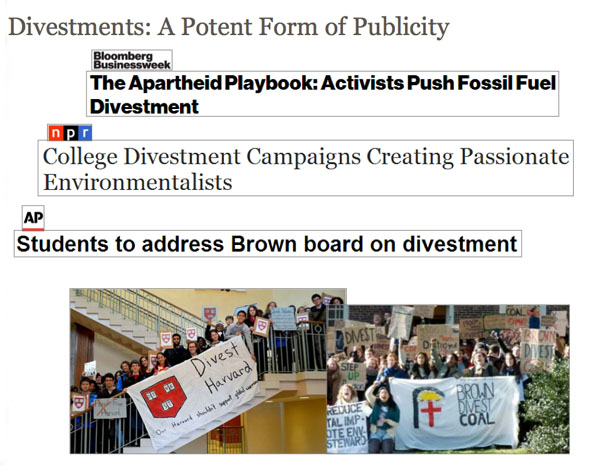
\includegraphics[width=100mm]{s7-divest-slide.png}
\centering
\caption{One slide from the slideshow on threats to the coal industry. Source: Meredith Xcelerated Marketing}
\label{fig:DivestSlide}
\end{figure}




Divestment would signal that the `smart money' is shifting away from fossil fuels. 
This could help produce a political climate in which significant action can be taken, including in the form of carbon pricing and reduced subsidies for fossil fuels.\footnote{See also: ``Companies like ExxonMobil, Shell, BP have billions of dollars/euros. How can divesting the funds from a few institutions like universities, pensions and churches make an impact?'' at: \url{http://gofossilfree.org/faq/}}


	
	\subsection{What are the University of Toronto's peer schools doing?}
	\label{PeerSchools}



Fossil fuel divestment campaigns are active at more than 300 schools across North America, including:
\begin{itemize}
	\item Harvard, Yale, Princeton, Stanford, MIT, Duke, Caltech, the University of Michigan, Tufts, Wellesley,
	\item The University of British Columbia, McGill, the University of New Brunswick--Fredericton, the University of Victoria, McMaster University, Concordia University, Simon Fraser University,
	\item and Oxford University.
\end{itemize}
To date, six universities and colleges have pledged to pursue fossil fuel divestment : San Francisco State University Foundation, Hampshire College, Unity College, Sterling College, College of the Atlantic, and Green Mountain College.\footnote{For a complete and up-to-date list, see: \url{http://campaigns.gofossilfree.org/}}



Divestment campaigns are active at many prominent American schools:
\begin{itemize}
	\item Divest \textbf{Harvard} has met with the university administration and with trustees to discuss divestment.\footcite[][]{HarvardMeeting} \footcite[][]{HarvardTrustees} On April 11th 2013, 1,300 petition signatures were delivered to the Harvard administration in support of divestment.\footcite[][]{HarvardPetition} 71 percent of students supported a referendum calling for fossil fuel divestment.\footcite[][]{StudentsClamoring}
	\item On May 30th 2013, the faculty senate at the \textbf{University of California}, Santa Barbara voted in favour of fossil fuel divestment. Earlier that week, the student government at Stanford University voted in favour of divestment. In total, the student governments at seven campuses of the University of California have voted in favour of divestment.\footcite[][]{UCSB2013}
	\item At \textbf{Stanford}, the undergraduate senate passed a resolution in support of fossil fuel divestment in May 2013.\footcite[][]{StanfordSenate}
	\item The president of \textbf{Tufts University} has established a working committee to consider fossil fuel divestment, as well as other steps the school could take to address climate change.\footcite[][]{TuftsDivest}
	\item \textbf{Hampshire College}, which was the first university to divest from South Africa during the 1980s, was also the first school to officially commit to fossil fuel divestment.\footcite[][]{StudentsClamoring}
\end{itemize}



Divestment is also being considered at schools across Canada:
\begin{itemize}
	\item The \textbf{McGill} divestment campaign is the most advanced of the Canadian divestment campaigns: the three major student unions have endorsed the divestment campaign, the petition was presented to the Board of Governors on February 1st, and was rejected on by the Board of Governors on May 23rd 2013.\footcite[][]{McGillStudentExecs} \footcite[][]{McGillDelivers}
	\item At the \textbf{University of New Brunswick}, students have collected over 300 signatures in support of divestment.\footcite[][]{UNBPetition} They have also submitted a presentation and resolution of support to the student union.\footcite[][]{UNBStudentUnion}
	\item At the \textbf{University of British Columbia}, students are calling on the UBC Investment Management Trust to sell the school's \$7.14 million in oil and gas investments.\footcite[][]{UBCDivest} In June 2013, UBC adopted a new responsible investment strategy.
\end{itemize}



No major university has yet committed to divest from fossil fuels.
This gives the University of Toronto an opportunity to distinguish itself and show leadership.
As the severity of climate change worsens, the case for divestment will strengthen; at the same time, as governments become more active it will become increasingly clear that fossil fuel stocks are overvalued.
By moving early, the University of Toronto can contain this risk and gain reputational advantages.



\subsubsection{Questions about divestment raised at other schools}



At other universities where fossil fuel divestment has been proposed, university administrations have responded with specific objections about the proposed course of action.
Toronto350.org's fossil fuel divestment proposal has been designed to take these considerations into account and this brief includes detailed responses to a number of counter-arguments.



At McGill, a proposal to divest from oil sands and fossil fuels was considered and rejected by the university administration in May 2013.\footnote{The proposal is available at: \url{http://Toronto350.org/brief/mcgill/the-social-injury-of-tar-sands-and-fossil-fuels.pdf} and the response is at: \url{http://Toronto350.org/brief/mcgill/camsr_documents_0.pdf}}
The issues raised by the McGill administration are addressed comprehensively in this brief.
For instance, the Report of the Committee to Advise on Matters of Social Responsibility states that:
\begin{quote}
In discussion with the Committee, the representatives of Divest McGill acknowledged they were unaware of examples of corporations involved in oil sands and fossil fuels which had been found to have violated or frustrated the enforcement of rules of domestic or international law intended to protect individuals against deprivation of health, safety or basic freedoms.\footcite[][p. 4]{McGillRejection}
\end{quote}
Two sections of this brief address this matter: \nameref{sec:FrustrateLaw} and \nameref{LegalPrecedents}



McGill's Committee to Advise on Matters of Social Responsibility also states that:
\begin{quote}
During the discussion, it was noted that a number of energy companies are actively engaged in research into and the production of alternate forms of energy, which suggests that investment in these companies may help to promote and encourage the use of alternate sources of energy.\footcite[][p. 4]{McGillRejection}
\end{quote}
This specific objection is addressed in: \nameref{RenewableInvest}



The committee at McGill also ``took note that the energy sector, including oil and gas extraction, production and distribution, is highly regulated by government at all levels''. This objection is considered in the section: \nameref{HeavilyRegulated}



In conclusion, the committee at McGill decided that:
\begin{quote}
While some members noted environmental and health effects related to the oil sands, the Committee found that Divest McGill had presented no evidence of a court finding of injury on the part of oil sands or fossil fuels companies, and otherwise had provided insufficient data and evidence to establish that social injury had occurred.\footcite[][p. 4]{McGillRejection}
\end{quote}
This brief provides detailed evidence of the social injury caused by fossil fuel companies, in the section: \nameref{sec:SocialInjury}.



Divestment as proposed by Toronto350.org is substantially more focused than what was presented by Divest McGill.
This proposal calls only for the sale of direct holdings in 200 listed companies, and does not call upon the university to identify firms involved in any specific fossil fuel related activity.
Furthermore, this proposal does not call for divestment from companies that make loans to the 200 companies listed.
This greatly simplifies the process of divestment, and removes any uncertainty about whether the firms in question are directly involved in the social injury described in this brief.



On June 4th 2013, the Board of Governors of the University of British Columbia (UBC) approved a new responsible investment strategy that included a number of objections to using divestment in response to concern about companies causing social injury.\footcite[][]{UBCRespInv}



The first concern raised is about the challenge of effectively screening potential investments according to environmental, social, and governance concerns:
\begin{quote}
Issues with portfolio screening are multiple and complex. Ethically, portfolio screening is difficult to apply to reflect the competing political, environmental and social interests playing out at any given time, and whether these interests should be company specific or sector-wide.
\end{quote}
This concern is eliminated in the approach proposed at the University of Toronto.
The list of companies where divestment is encouraged is already prepared and included in: \nameref{sec:200Companies}.
Since these are the 200 global companies with the largest fossil fuel reserves, there is a direct logical reason why they each is included in the list.
This pertains both to the degree of social injury that would be caused by the burning of their reserves, as well as the degree of regulatory risk involved in investing in these firms, given the growing willingness of governments to regulate GHG pollution.



Another issue raised in the UBC document is:
\begin{quote}
Economically, screening out entire sectors such as the Canadian energy sector would push more of the endowment outside of the country, into geographic areas that often have more questionable social and environmental records.
\end{quote}
The 200 companies listed in this proposal are global, mitigating the risk that U of T would shift its endowment into more damaging companies elsewhere.
This brief also includes a response to the concern: \nameref{CanadianJobsEconomy}



The last objection to divestment included in the UBC document is:
\begin{quote}
Financially, implementing a direct screening policy would prevent UBC from investing in pooled or indexed funds and would generate significant overhead that would negatively impact student and researchers supported by the endowment.
\end{quote}
Once again, this concern does not apply to the approach proposed by Toronto350.org, which calls only for divestment of direct stock holdings at this time.



	\subsection{What are other large investors doing?}
	\label{LargeInvestors}



Several cities are considering divesting themselves from fossil fuel stocks.\footnote{See: \url{http://gofossilfree.org/commitments/}}
The mayor of Seattle has called for the city to divest its fund for daily operations (US\$1.4 billion), its deferred compensation plan (US\$700 million), and its pension system (US\$1.9 billion).\footcite[][]{SeattleDivest}
The mayor of Portland, Oregon has urged the Oregon State Treasurer, the Local Government Investment Pool, and the Oregon Investment Council to divest all state holdings in fossil fuel companies.
The San Francisco Board of Supervisors has urged the retirement board to divest US\$583 million of fossil fuel holdings in the city's \$16 billion retirement fund.\footcite[][]{DivestProtect40to60}
In June 2013, the city council of Providence, Rhode Island voted 11-1 in favour of divestment.\footcite[][]{ProvidenceDivest}



Eleven regional conferences of the United Church of Christ in the United States have voted to divest.\footcite[][]{ChurchesFFDivestment}
Numerous other churches and faith-based organizations are considering divestment, including the First Unitarian Church of Salt Lake City, the Evangelical Lutheran Church of Oregon, and the Uniting Church of New South Wales \& ACT, Australia.



Hedge fund billionaire Tom Steyer has decided to divest his holdings in fossil fuel companies.
He thinks that a portfolio that excludes fossil fuels ``will outperform the market''.\footcite[][]{SteyerMiddleburyLetter}
In July 2013, the Norwegian financial services company Storebrand ASA announced that they will be divesting from 19 fossil fuel companies.\footcite[][]{StorebrandPR}
The decision was motivated by the belief that the value of these companies would fall because of their negative climate change impacts.\footcite[][]{StorebrandNews} \footcite[See also: ][]{GristStorebrand}
The Dutch bank Rabobank has also decided not to fund shale oil development.\footcite[][]{RabobankRefuses}
According to a spokesperson from the bank, this is because ``[t]he bank's global policy is not to be involved with extracting fossil fuels where it is not clear what the risks and consequences may be''.\footcite[][]{RabobankNews}



In July 2013, European Union Climate Commissioner Connie Hedegaard called for the European Investment Bank (EIB), the European Bank for Reconstruction and Development (EBRD), and the World Bank to eliminate public support for fossil fuels.\footcite[][p. 9--10]{InvestHasteRepent} \footcite[See also:][]{HedegaardAppeal}
Each year, these three institutions provide US\$168 billion in funding for projects around the world.\footcite[][p. 10]{InvestHasteRepent}


	
	\subsection{But don't fossil fuel companies also invest in renewable energy?}
	\label{RenewableInvest}



In 2008, British Petroleum (BP) launched a rebranding effort in which it claimed that its initials now meant `Beyond Petroleum'.\footcite[][]{GreenwashBP}
This is now widely seen as an example of `greenwashing' --- a practice defined as devoting extensive resources to advertising how environmentally-friendly an organization claims to be, while not actually adopting sustainable practices.\footnote{The Oxford English Dictionary defines the term as: ``The creation or propagation of an unfounded or misleading environmentalist image''}
BP has since abandoned its foray into solar power generation and put its U.S. wind-farm business up for sale.\footcite[][]{BPNoLongerBeyond} \footcite[][]{BPNoMore}
This behavious is typical of the fossil fuel industry, which has spent vast sums of money touting its environmental credentials, at the same time as their business plans --- which depend on burning all of their fossil fuel reserves --- are fundamentally at odds with environmental sustainability.
As BP's chief executive, John Browne spent \$200 million advertising the `Beyond Petroleum' slogan.
Under his tenure, BP was ``marred by a succession of devastating accidents... [including] an explosion at BP's Texas City refinery in 2005 that killed 15 workers and injured 170 others, and an oil spill a year later that dumped 4,800 barrels of oil at Prudhoe Bay, on the coast of Alaska''.\footcite[][]{BlackStuffBP}
In April 2010, BP's Deepwater Horizon oil platform in the Gulf of Mexico exploded, causing over \$40 billion in damage, alongside massive ecological harm.\footcite[][]{OffshoreLiability}
All told, BP may end up paying over US\$90 billion in fines and compensation for causing the disaster.\footcite[][p. 20]{Supermajordammerung}
At the peak, BP was directing 6 percent of overall investment toward renewables.
This compares with 2.5 percent at Chevron and Shell, with no other major oil company investing more than 1 percent.\footcite[][]{RSBigOilLies}



The sums being invested in renewable energy by fossil fuel companies are dwarfed by the investments they are making in unconventional sources of coal, oil, and gas.
For example, BP has announced its intention to increase spending on arctic drilling by \$1 billion over five years, increasing its fleet of oil rigs from seven to nine by 2016.\footcite[][]{BPArcticBillion}
In 2003, BP invested \$6.75 billion in Russia's Tyumen Oil Company, which is involved with the massive Sakhalin offshore project.\footcite[][]{NotBeyondInRussia}
In total, the Government of Alberta expects over \$218 billion to be invested in the oil sands over the next 25 years.\footcite[][]{OilSandsEconBenef}
The 200 fossil fuel companies with the largest reserves spent \$674 billion in 2012 identifying and developing new fossil fuel reserves, as well as researching ways to extract fossil fuels from proven reserves.\footcite[][p. 4]{CTI2012} \footcite[See also: ][]{SteinerFinancialSector}



Conventional fossil fuel sources are more than sufficiently abundant to allow humanity to far exceed the 2˚C `safe limit' for climate change.
The costly pursuit of exotic new reserves shows how fossil fuel companies have failed to internalize the reality of climate change and are continuing to implement investment plans that are sharply at odds with planetary safety.
Also, based on various credible estimates of the social cost of carbon, the total damage being done to society by fossil fuel burning substantially exceeds the scale of the investments the industry is making in renewables.\footnote{See: \nameref{sec:PricingSocialCost}}

	
	
	\subsection{In what cases have courts found that fossil fuel companies caused injury?}
	\label{LegalPrecedents}
	
	
	
So far, there are a limited number of legal precedents in which the seriousness of climate change and the injury being caused by fossil fuel companies are recognized.
Those that exist can be found in: \nameref{sec:FrustrateLaw}.
The Supreme Court of British Columbia decision ``Tsilhqot'in Nation v. British Columbia'' acknowledges climate change impacts on mountain pine beetles, and on biodiversity generally.\footcite[][p. 358, 406]{Tsilhqotin}


In past instances, the University of Toronto has accepted the appropriateness of divestment before a comprehensive legal justification has been in place.


\begin{vcom}
Find information about how U of T divested from South Africa before Canada passed the law to facilitate that. Also, the tobacco precedent.
\end{vcom}


\begin{vcom}
* Legal efforts by small island states
* One example: https://www.sindark.com/2008/09/14/carbon-emissions-worse-than-criminal-damage/
* Fossil fuel companies also cause injury in forms other than climate
* Oil spills - Deepwater Horizon
* Toxic air pollution - deaths from coal
* This guy might be able to make some suggestions: http://www.law.columbia.edu/courses/L8451-advanced-climate-change-law/spring-2013/section-001
* Also: http://envirolaw.com/about/meet-dianne/
\end{vcom}
	
	
	
	\subsection{Isn't the energy sector, including oil and gas extraction, production and distribution, highly regulated by government at all levels?}
	\label{HeavilyRegulated}
	


When it comes to GHG pollution, the fossil fuel industry is essentially unregulated at the federal level in Canada.
Firms are free to use the atmosphere as a dumping ground for \ce{CO2} pollution.\footcite[See: ][]{Paris2013} \footcite[See also: ][]{Stewart2013}
The harm the industry is causing is largely dispersed, which makes it hard to assign responsibility, but we know there are major damaging impacts in the aggregate.



Not only that, but many governments in Canada have adopted policies intended to accelerate the growth of the fossil fuel sector.
These include aggressive international lobbying for oil pipelines and other forms of fossil fuel export infrastructure.\footcite[See, for example: ][]{KeystoneLobbyingHarder} \footcite[][]{HarperNoBrainer} \footcite[][]{OliverRadicalLetter}
They also include steps to weaken environmental assessment processes, reduce the scope of scientific research being conducted on climate change while suppressing the publication of results from government scientists, and substantial continuing subsidies to the fossil fuel industry.



The regulation that exists in Canada is not putting the country on a pathway toward making a fair contribution in the global climate change mitigation effort.
Additional regulation is required and --- until it is in place --- socially conscious organizations should take action themselves in response to the harm being caused by fossil fuels.


	
	\subsection{Can humanity manage without fossil fuels?}
	\label{DoingWithout}



This question was extensively examined by Cambridge physicist David MacKay, resulting in his 2009 book \emph{Sustainable Energy – without the hot air}, which is available for free online.\footcite[][]{MacKay2009}
In his detailed analysis, MacKay considers both the scope for reducing energy demand through energy efficiency and the opportunities for producing energy from low- and zero-carbon sources like renewables and nuclear power.
In order to demonstrate the feasibility of providing everyone in the world with enough energy to sustain a high standard of living, MacKay calculates that ``[t]o supply every person in the world with an average European's power consumption (125 kWh/d [kilowatt-hours per day]), the area required would be two 1000 km by 1000 km squares in the desert''.\footcite[][p. 178]{MacKay2009}
Although doing this with only giant solar facilities would be impractical and probably expensive, the example nonetheless demonstrates that humanity can enjoy an improved standard of living without relying on fossil fuels at all.
MacKay concludes that by combining wind, hydro, tidal, wave, geothermal, solar, and nuclear power it is possible for everyone in the world to consume 80 kWh per day --- equivalent to the total per capita energy use in Hong Kong today.\footcite[][p. 106, 238]{MacKay2009}



The opportunities associated with renewable energy deployment are already being realized, and major growth potential remains.
The U.S. Department of Energy believes that by 2030, 20 percent of American electricity could come from wind, reducing annual electric sector \ce{CO2} emissions by 825 million metric tons.\footcite[][]{20PercentBy2030}
Iowa already generates 39 percent of its energy from this low-carbon source.\footcite[][]{BlownAway}
Concerns about the intermittency of wind energy have also proven exaggerated; by balancing production from wind facilities in different areas, consistent power output can be created.\footcite[][]{BlownAway}



Huge opportunities exist to reduce energy use by improving efficiency, including in industry, transport, power generation, and buildings.
According to the International Energy Agency (IEA), these possibilities have not yet been factored into government planning: ``[t]wo-thirds of the economic potential to improve energy efficiency remains untapped in the period to 2035'' and energy efficiency remains ``a huge opportunity going unrealised''.\footcite[][p. 13]{IEA2012press}
The IEA explains that ``[e]conomically viable efficiency measures can halve energy demand growth to 2035'' and produce reductions in oil use equivalent to the production from Russia and Norway.\footcite[][p. 14]{IEA2012press}
By 2035, the IEA predicts that improved energy efficiency could cut energy expenditures by 20 percent, alongside ``wider economic gains, particularly for India, China, the United States and Europe''.\footcite[][p. 15]{IEA2012press}



The transition to renewable energy will bring jobs and other economic benefits.
Analysis from the Union of Concerned Scientists found that a national standard of 25 percent renewable energy in the United States by 2025 would ``create more `green' jobs, lower consumer energy bills in every region of the country, and reduce carbon dioxide (\ce{CO2}) and other harmful emissions from power plants—the biggest source of global warming pollution in the United States.''\footcite[][]{ConcernedScientistsJobs}
The report finds that this policy would create three times as many jobs as producing the same amount of energy from fossil fuels.\footcite[See also: ][]{CSBenefitsRenewable}
A zero-carbon energy system would also reduce volatility in energy prices, since the inputs are free once the infrastructure is built, and would eliminate the security and economic risks experienced by states dependent on fossil fuel imports.



On a business-as-usual pathway in which humanity burns most or all of the planet's remaining fossil fuels, the planet can be expected to experience catastrophic changes that will wreak considerable economic damage.
As such, the choice we are facing is not between perpetuating the \emph{status quo} indefinitely or committing to decarbonization.
Rather, our choice is between decarbonization and catastrophic climate change.
The World Bank has argued that ``[t]he current level of action puts us on a pathway towards a 3.5–4°C warmer world by the end of this century'' and that ``[s]uch a scenario would have a devastating impact on the climate and would threaten our current economic model with unprecedented and unpredictable impacts on human life and ecosystems in the long term.''\footcite[][p. 13]{WorldBankCarbonPricing} \footcite[See also:][]{WoesReverse}
As the Australian government's Climate Commission explains: ``Burning all fossil fuel reserves would lead to unprecedented changes in climate so severe that they will challenge the existence of our society as we know it today.''\footcite[][p. 5]{CriticalDecade2013}


Whether we like it or not, humanity must learn how to manage without fossil fuels.



	\subsection{Won't divestment hurt the endowment, including U of T's ability to provide scholarships?}
	\label{HurtEndowment}
	
	
	
As discussed at greater length in \nameref{NoDivestPenalty}, there is evidence that portfolios that exclude companies that cause social injury do not suffer a financial penalty for doing so.
Deutsche Bank and Mercer have conducted major meta-studies on portfolios that consider environmental, social and governance (ESG) factors and found that there is either a neutral or positive relationships between financial performance and the incorporation of ESG factors into portfolio management.\footcite{DeutscheBankSI} \footcite{MercerRI}
Hedge fund billionaire Tom Steyer explains in a letter to the Corporation of Brown University:
\begin{quote}
The available research, looking backward, shows that the return penalty would be tiny—but in any event good investors rarely look backward. Looking to the future, the data on climate change makes it clear that something has changed, and as the rest of the world realizes this, coal stocks will come under increasing pressure. At the moment, other investors have not fully realized the risk that carbon reserves will become a stranded asset; if you acknowledge what your own science departments are telling you this gives you an edge relative to those investors. I can tell you that in my own investments, I have directed my financial team to divest my holdings of coal investments so that I will have a coal free portfolio myself – in part because I am convinced it will outperform the market.\footcite[][]{SteyerBrownLetter} \footcite[See also: ][]{SteyerMiddleburyLetter}
\end{quote}
Unlike fossil fuel divestment, failing to deal with the `carbon bubble' could harm the university's financial standing in the long term.



Universities are entities that expect to exist forever and which therefore have very long time horizons for their investment decisions.
In the long term, the university's ability to fund research and provide scholarships depends on general financial health, which would be improved by divestment.




	\subsection{Won't fossil fuel companies stop making donations to U of T?}
	\label{NoMoreDonations}



Donations from fossil fuel companies are reasonably limited. 
For instance, `President's Circle' donors who have given over \$1,827 annually include Husky Energy, the Imperial Oil Foundation, the Mitsui Canada Foundation, Petro-Canada (a subsidiary of Suncor), RioTinto Alcan, and Shell Canada.\footnote{See: \url{http://boundless.utoronto.ca/member-listing/}}
The full list includes several hundred donors.
Three fossil fuel companies have also participated in the university's Boundless campaign: Husky Energy Inc., RioTinto Alcan, and the Mitsui Canada Foundation.\footnote{See: \url{http://boundless.utoronto.ca/member-listing/}}
Once again, the list includes a dominant share of non-fossil-fuel-corporation donors.



These donations do not offset the financial risks associated with heavy investment in fossil fuels, nor do they compensate for the ways in which fossil fuel investments are contrary to the university's values and policies.



Two major motivations for corporate donations to the university are advertising and positive publicity.
Neither of these objectives would be undermined by divestment, so it is plausible that corporate donations from fossil fuel companies could continue in spite of divestment.



When Unity College divested, they experienced an uptick in applications and donations.\footcite[][p. 4]{CaseForDivestment}



	\subsection{Shouldn't U of T fight climate change through research and education?}
	\label{ResearchEducation}



U of T is active in climate change research and teaching, and this will continue.\footnote{See: \nameref{UofTAcademicProgramming}}
This research has helped to establish what a serious and pressing problem climate change is for people in Canada and around the world.
Although this work is very welcome, it is not a substitute for divestment.
The very existence of the divestment policy shows that the university has accepted the basic argument that some investments can be incompatible with the values of the university.



	\subsection{Won't divestment hurt Canadian jobs and the economy?}
	\label{CanadianJobsEconomy}
	
	

This question gets the argument backwards: not dealing with climate change could cause enormous harm to Canadian prosperity.
At the same time, there are major risks associated with continuing to invest hugely in fossil fuel infrastructure, at a time when the policy-makers of the world are starting to get serious about controlling climate change.
As detailed extensively in section 3 (\nameref{sec:SocialInjury}), climate change poses a serious risk to Canadian prosperity. 
Furthermore, as detailed in section 4 (\nameref{sec:Fiduciary}), there are major risks associated with continuing to invest in fossil fuel projects.


Right now, the Canadian economy is excessively dependent on fossil fuel production and export.
Canada also has excessively high \emph{per-capita} emissions of GHG pollution - meaning we will probably need to cut faster and deeper than most, as part of a fair global transition to a low-carbon economy.
Given that the future will be carbon-constrained, it is urgent that we start mitigating that dependence.
Divestment by the University of Toronto would send an important signal to help initiate this necessary transition.
As highlighted in the Stern Review: ``The benefits of strong, early action on climate change outweigh the costs''.\footcite[][p. i]{Stern2007}
Early divestment could also help reduce the risk of large amounts of investment being tied up in fossil fuel projects that will need to be shut down before the end of their economic lives as global and Canadian restrictions on GHG pollution are tightened.



Furthermore, as the world gets serious about decarbonization, extensive economic opportunities will arise in this sector.
These will include the retrofitting of buildings to improve efficiency, the construction of renewable energy infrastructure, and research and development to support and enhance the transition.
As a key research institution, U of T can participate directly in that part of the world's economic realignment.



	\subsection{Can't we just adapt to climate change?}
	\label{WhyNotAdapt}



As described at considerable length in section 3 (\nameref{sec:SocialInjury}), the impacts of even 2˚C of climate change would be severe, and a business-as-usual pathway in which we continue to use fossil fuels the way we do now would likely see temperatures up more than 5˚C by 2100.


There is no adapting to climate change that melts the Greenland and West Antarctic ice sheets, flooding huge populated areas.
Similarly, climate change on such a scale would be accompanied by an acute risk of abrupt and irreversible effects.
In order to have a reasonable chance of adaption that leads to a world with comparable human prosperity to what we enjoy now, climate change must be kept under 2˚C.
That means most of the world's fossil fuels cannot be burned, leading to the various implications described in this brief.



	\subsection{Won't carbon capture and storage (CCS) save us?}
	\label{CCSSaves}



Carbon capture and storage (also called carbon capture and sequestration) is a technology that promises to separate \ce{CO2} from the emissions of facilities like power plants and bury it in underground formations such as saline aquifers.
The technology has already been deployed in certain applications, such as the re-injection of unwanted \ce{CO2} Sleipner gasfield in Norway.



CCS cannot solve our climate change problem for two major reasons: scale and economics.



Humanity is now emitting roughly 30 billion tonnes of \ce{CO2} into the atmosphere annually.\footcite[][]{RedrawingClimateEnergy}
As explained in an article in the \emph{MIT Technology Review}: ``[I]f we were to bury just one-fifth of the global carbon dioxide emissions, we would need to build an industry capable of handling twice the volume of stuff as the entire oil industry, an industry that took 100 years to develop, driven by a large and mostly expanding market.''\footcite[][]{BullisonCCS}
Rather than being a genuine means for dealing with climate change, CCS has more often been a way for the fossil fuel industry to delay serious government action by claiming that a wonderful technological solution will soon exist.
This claim is at odds with the difficulties encountered by test projects like FutureGen --- a supposedly `clean' coal-fired power plant announced by President George W. Bush in 2003, but which was subsequently scrapped because of intolerably high costs.
As \emph{The Economist} explains: ``there is not a single big power plant using CCS anywhere in the world''.\footcite[][]{TroubleInStore}



On the economics of CCS, \emph{The Economist} explains:
\begin{quote}
The problem with CCS is the cost. The chemical steps in the capture consume energy, as do the compression and transport of the carbon dioxide. That will use up a quarter or more of the output of a power station fitted with CCS, according to most estimates. So plants with CCS will need to be at least a third bigger than normal ones to generate the same net amount of power, and will also consume at least a third more fuel. In addition, there is the extra expense of building the capture plant and the injection pipelines. If the storage site is far from the power plant, yet more energy will be needed to move the carbon dioxide.\footcite[][]{TroubleInStore}
\end{quote}
Despite considerable government subsidies, including \$3.4 billion in an Americans stimulus bill, CCS remains unattractive to energy utilities largely because of cost.\footcite[][]{IllusionCleanCoal}
In a discussion paper published by the Belfer Center for Science and International Affairs at Harvard, it was estimated that sequestering one tonne of \ce{CO2} would cost approximately \$150 --- far more than the cost of avoiding the emissions in the first place by implementing lower-cost measures.\footcite[][]{RealisticCostsCarbonCapture}



Other considerations include the stability of formations into which \ce{CO2} is injected and the seismic consequences of doing so.\footcite[][]{CCSEarthquake} \footcite[See also: ][]{AFPonCCS}
Carbon dioxide is heavier than air, so leaks from CCS facilities could smother people and animals nearby.\footcite[][]{TroubleInStore}
Water saturated with \ce{CO2} also becomes acidic, which could undermine the integrity of equipment and underground formations intended to contain it.
CCS is also useless for mobile sources of emissions where \ce{CO2} cannot plausibly be separated from waste gases and stored.
Given that 85 percent of the total emissions associated with fuels from the oil sands occur when the fuels are burned in vehicles, this means the scope for decreasing the climate impact of the oil sands with CCS is especially limited.\footcite[][]{HardToScrub} \footcite[][]{NoSilverBullet}



The failure of CCS to live up to its promise is especially problematic for Canada, given the degree to which the climate change plans of the federal government and the Government of Alberta depend on this technology becoming cheap and effective in the near term.
Canada's unrealistic expectations for CCS mean that decarbonization will be even more challenging than expected by the federal and provincial governments, making it all the more important to begin investing in decarbonization now.



	\subsection{Won't geoengineering save us?}
	\label{GeoSaves}
	
	
Geoengineering is the deliberate modification of the climate system, intended to counteract the effect of anthropogenic climate change.
Several different mechanisms for achieving this have been proposed, but all are deeply problematic for a variety of reasons.
Geoengineering mechanisms can be broadly broken down into those that would seek to reduce global temperatures without lowering atmospheric \ce{CO2} concentrations and those that would actually seek to draw \ce{CO2} from the atmosphere.



The latter sort --- which could theoretically reduce the atmospheric concentration of GHGs --- suffer from the same problems of scale and economics experienced by CCS, exacerbated by the additional cost of separating \ce{CO2} from air (where it is relatively low in concentration) rather than directly from the waste stream of power plants and other facilities where it is relatively concentrated.  



The former sort, which could be achieved through means like injecting large volumes of sulfate aerosols into the upper atmosphere, suffers from even more significant problems.
For one thing, it would do nothing to stop the acidification of the world's oceans: a trend that threatens to destroy the ability of marine organisms to form shells and skeletons from calcium, along with other unknown global effects on marine food webs.
For another, geoengineering of this type would be likely to further alter global precipitation patterns, in addition to the changes that would be created by climate change.
This sort of intervention would also need to be undertaken constantly and forever; if it were to be discontinued, global temperatures would spike.



In short, geoengineering adds new risks on top of those from climate change, there is no guarantee it would be effective in reducing global temperatures and addressing the other consequences of climate change, and it would be likely to bring significant side-effects.
Choosing to geoengineer would mean choosing to impose even more risk and damage upon future generations than we already are.



% END SECTION 7

% END SECTION 7



% BEGIN SECTION 8
% BIBLIOGRAPHY

% BEGIN SECTION 8
% Last updated by Milan Ilnyckyj 2013-06-14

% If encountering problems with sources rendering correctly, check to make sure all the proper commas are in place and that symbols like \$ and \& are written properly for LaTeX



	\singlespacing
	\section{Sources cited}
	\label{sec:Sources}
	\doublespacing



\nocite{DoreDisaster}



\printbibliography



% END SECTION 8

% END SECTION 8



% BEGIN SECTION 9
% DIVESTMENT POLICY

% BEGIN APPENDIX I
% Last updated by Milan Ilnyckyj 2013-07-06



		\singlespacing
		\section{Appendix I: Issues with respect to university divestment}
		\label{sec:DivestmentPolicy}
		\doublespacing
		
		
		
	\subsection{Policy on Social and Political Issues With Respect to University Divestment}
	\label{PolicySocialPolitical}

	
	
March 4, 2008



\textbf{Preamble}

 

The University's core academic values include freedom of inquiry and open debate. As a general matter, the University does not take positions on social or political issues apart from those directly pertinent to higher education and academic research.  Instead, its role is to provide a forum within which issues can be studied carefully and debated vigorously. Given these values, the University will not consider any proposals for restrictions on its investments that require the institution to take sides in matters that are properly the subject of ongoing academic inquiry and debate.

 

As a corollary, the University's response to any petition regarding divestment must be governed by the fundamental place of diversity of opinion within its community. Except in those situations in which the University must settle on an answer to controversial questions about how best to achieve its academic mission, the University risks abandoning its core values if it takes sides in ongoing debates and is perceived to be advancing a specific political or social position.



\textbf{Principles}

 

In responding to questions about social and political issues with respect to University investment, it is acknowledged that first and foremost, maximizing economic return consistent with the University’s stated risk tolerance should be the criterion for purchase and sale of stock in all normal circumstances. In specific instances where the University's social responsibility as an investor is questioned, however, credible and effective procedures for responding should exist.

 

Responses should be based on the following principles:



(i) prudent investment. The University has a fiduciary duty to manage investments responsibly to maximize return on its investments within a policy risk tolerance as approved by Business Board from time to time.

 


(ii) the Yale University concept of social injury:

 

(a) Social injury is the injurious impact which the activities of a company are found to have on consumers, employees, or other persons, particularly including activities which violate, or frustrate the enforcement of, rules of domestic or international law intended to protect individuals against deprivation or [sic] health, safety, or basic freedoms; for purposes of this Policy, social injury shall not consist of doing business with other companies which are themselves engaged in socially injurious activities.

 

(iii) actions taken by the Canadian government or other national or international bodies with regard to the particular issue of concern.

 

Consideration of questions about social and political issues with respect to University investment must take into account applicable legislative requirements and government or University policy, as well as the legal standards applicable to prudent institutional investors.




\textbf{Advisory Committee}

 

The President will establish an \emph{ad hoc} committee of qualified individuals to review any investments claimed to be in conflict with University’s social and political positions and to advise the President on possible actions to be taken.  Chaired by a senior University officer designated by the President, the committee will consist of individuals with relevant expertise from among the teaching staff, students, administrative staff and alumni.  The Executive Committee of the Governing Council will be asked to approve the appointments on the recommendation of the President.

 

In making recommendations regarding the membership, the President will take into account any potential conflicts of interest proposed members might be expected to have with a view to minimizing such conflicts of interest on the part of committee members

 

The committee’s report and the President’s decision will be reported to the Governing Council through the Executive Committee.

 

The President will issue procedures regarding the implementation of this policy. The first such procedures are included here for information, and the President will review any substantive changes in those procedures with the Executive Committee of the Governing Council.
	


\clearpage


	
	\subsection{Procedures for Responding to Social and Political Issues with Respect to University Divestment}
	\label{ProceduresResponding}
	
	
January 2008


\textbf{Raising Issues}

 

Members of the University of Toronto community who wish to raise issues with regard to University investments that are in conflict with stated University policies may do so by:
\begin{itemize}
	\item preparing a convincing brief establishing the case; and
	\item presenting the evidence of general concern in the University community by collection of signatures.
\end{itemize}
Responsibility for initiating a request for University action regarding its investments rests with members of the University community. One or more individuals must prepare a fully documented brief identifying the social or political issue that they believe requires divestment.

 

When the brief has been fully prepared, the initiators of the request must secure evidence of support for their cause through the collection of at least 300 signatures endorsing the brief. Up to 200 of the signatures could come from a single constituency of the University community (for the purposes of these procedures, the constituencies are teaching staff, students, administrative staff, and alumni); the remaining 100 signatures must be from at least two other University constituencies with a minimum of 25 signatures from any individual constituency.  Each signatory must attest that he/she has read and agrees with the entire content of the brief.

 

When signatures have been added to the brief, the material is to be deposited with the office of the President.

 

\textbf{Response}

 

The administration will respond by establishing an \emph{ad hoc} review committee as specified by the policy.

 

This committee, chaired by a senior officer designated by the President, will consider the briefs. The committee may consult with investment and other experts as they deem necessary.

 

If the committee determines that the brief repeats previous submissions, or is vexatious or frivolous, it will cease its deliberations and recommend to the President that the brief be dismissed. If the brief is not repetitive, vexatious or frivolous, the committee shall complete its deliberations and provide its recommendation in writing to the President regarding the appropriate action to be taken by the University.

 

The committee will consider the following guidelines in considering the appropriate response to any request:
\begin{itemize}
 	\item the extent and significance of the University's investment in a particular entity.  Determination of whether investments are considered significant will depend on the committee’s judgment of the relative magnitude of the University’s holdings both as a fraction of all University investments and in relation to the market capitalization of the entity under review.
	\item the degree to which the entity itself is involved in the undesirable activity.
\end{itemize}
Normally, activity is considered significant if more than ten percent of the entity's revenues are derived from the undesirable activity.

 

The President will consider the recommendations and make the final decision.

 

\textbf{Reporting}

 

The written report and the President's decision will be provided to the Governing Council through the Executive Committee. Following receipt of the report and the President’s decision by the Governing Council, the report and decision will be provided to the petitioners.

\emph{Approved by Governing Council on March 4, 2008, replacing the Policy on Social and Political Issues with Respect to University Investment revised and approved by the Governing Council on December 14, 1994.}

% END APPENDIX I

% END SECTION 9



% BEGIN SECTION 10
% LIST OF COMPANIES

% BEGIN APPENDIX II - STUART
% Last updated by Milan Ilnyckyj 2013-06-24



		\singlespacing
		\section {Appendix II: The 200 companies with the largest fossil fuel reserves}
		\label{sec:200Companies}
		\doublespacing



Toronto350.org is asking the University of Toronto to divest from direct stock holdings the following 200 companies, as listed in the Carbon Tracker Initiative's 2012 report, \emph{Unburnable Carbon}.\footcite{CTI2012} 
These are the top 200 listed companies ranked by estimated carbon reserves.



\begin{itemize}
  \item African Rainbow Minerals Ltd.
  \item AGL Energy
  \item Alcoa Inc.
  \item Allete Inc.
  \item Alliance Resource Partners L.P.
  \item Alpha Natural Resources Inc.
  \item Anadarko Petroleum Corp.
  \item Anglo American PLC
  \item Apache Corp.
  \item Aquila Resources Ltd.
  \item Arc Resources Ltd.
  \item ArcelorMittal
  \item Arch Coal Inc.
  \item Aston Resources Pty Ltd.
  \item ATP Oil \& Gas Corp.
  \item Bandanna Energy Ltd.
  \item Bankers Petroleum Ltd.
  \item Banpu PCL
  \item Bashneft
  \item Baytex Energy Corp.
  \item Berry Petroleum Co. (Cl A)
  \item BG Group PLC
  \item BHP Billiton
  \item Black Hills Corp.
  \item Bonavista Energy Corp
  \item BP PLC
  \item Bumi Resources
  \item Cairn Energy PLC
  \item Canadian Natural Resources Ltd.
  \item Canadian Oil Sands Ltd.
  \item Capital Power Corp.
  \item Cenovus Energy Inc.
  \item Chesapeake Energy Corp.
  \item Chevron Corp.
  \item China Shenhua Energy Co. Ltd.
  \item Churchill Mining PLC
  \item Cimarex Energy Co.
  \item Cliffs Natural Resources Inc.
  \item Cloud Peak Energy Inc.
  \item CLP Holdings Ltd.
  \item CNOOC Ltd.
  \item Coal India Ltd.
  \item Coal of Africa Ltd.
  \item Compania Espanola de Petroleos S.A.
  \item Concho Resources Inc.
  \item ConocoPhillips
  \item Consol Energy Inc.
  \item Continental Resources Inc. Oklahoma
  \item Crescent Point Energy Corp.
  \item Datang International Power Generation Co. Ltd.
  \item Datong Coal Industry Co. Ltd.
  \item Denbury Resources Inc.
  \item Devon Energy Corp.
  \item Ecopetrol S.A.
  \item El Paso Corp.
  \item EnCana Corp.
  \item Energen Corp.
  \item Enerplus Corp.
  \item ENI S.p.A.
  \item EOG Resources Inc.
  \item EQT Corp.
  \item Eurasian Natural Resources Corp. PLC
  \item Evraz Group S.A.
  \item Exxaro Resources Ltd.
  \item Exxon Mobil Corp.
  \item FirstEnergy Corp.
  \item Forest Oil Corp.
  \item Fortune Minerals Ltd.
  \item Fushan International Energy Group Ltd.
  \item Gansu Jingyuan Coal Industry \& Electricity Power 
  \item Gazprom OAO
  \item GDF Suez S.A.
  \item Global Energy Development PLC
  \item Grupo Mexico S.A.B. de C.V.
  \item Gujarat NRE Coke Ltd.
  \item Gujarat NRE Coking Coal Ltd.
  \item Hess Corp.
  \item Homeland Energy Group Ltd.
  \item Huolinhe Opencut Coal Industry Corp. Ltd.
  \item Husky Energy Inc.
  \item Idemitsu Kosan Co. Ltd.
  \item Imperial Oil Ltd.
  \item INA-Industrija Nafte
  \item Inner Mongolia Yitai Coal Co. Ltd.
  \item Inpex Corp.
  \item International Coal Group Inc.
  \item Irkutskenergo
  \item Itochu Corp.
  \item James River Coal Co.
  \item Jindal Steel \& Power Ltd.
  \item Jizhong Energy Resources Co. Ltd.
  \item Kazakhmys PLC
  \item Kuzbassenergo
  \item Linn Energy LLC
  \item Lukoil Holdings
  \item Lundin Petroleum AB
  \item Macarthur Coal Pty Ltd.
  \item Magnitogorsk Iron \& Steel Works
  \item Marathon Oil Corp.
  \item Mariner Energy
  \item Massey Energy Co.
  \item Mechel OAO
  \item Mitsubishi Corp.
  \item Mitsui \& Co. Ltd.
  \item Mitsui Matsushima Co. Ltd.
  \item MOL Hungarian Oil and Gas Plc
  \item Mongolian Mining Corp.
  \item Murphy Oil Corp.
  \item NACCO Industries Inc. (Cl A)
  \item New Hope Corp. Ltd.
  \item New World Resources N.V.
  \item Newfield Exploration Co.
  \item Nexen Inc.
  \item Neyveli Lignite Corp. Ltd.
  \item Noble Energy Inc.
  \item Noble Group Ltd
  \item Northern Energy Corp. Ltd.
  \item Novatek
  \item Novolipetsk Steel OJSC
  \item NTPC Ltd.
  \item Occidental Petroleum Corp.
  \item Oil \& Natural Gas Corp. Ltd.
  \item Oil India Ltd.
  \item Oil Search Ltd.
  \item OMV AG
  \item Optimum Coal Holdings Ltd.
  \item PA Resources AB
  \item Pacific Rubiales Energy Corp.
  \item Patriot Coal Corp.
  \item Peabody Energy Corp.
  \item Pengrowth Energy Corp.
  \item Penn West Petroleum Ltd.
  \item PetroBakken Energy Ltd.
  \item Petrobank Energy \& Resources Ltd.
  \item Petrobras
  \item Petroleum Development Corp.
  \item Pingdingshan Tianan Coal Mining Co. Ltd.
  \item Pioneer Natural Resources Co.
  \item Plains Exploration \& Production Co.
  \item Polo Resources Ltd.
  \item Polyus Gold OAO
  \item Premier Oil PLC
  \item Prophecy Resource Corp.
  \item PT Adaro Energy
  \item PT Bayan Resources
  \item PTT PCL
  \item Public Power Corp. S.A.
  \item Questar Corp.
  \item Quicksilver Resources Inc.
  \item Range Resources Corp.
  \item Raspadskaya OJSC
  \item Repsol YPF S.A.
  \item Resolute Energy Corp.
  \item Rio Tinto
  \item Rosneft
  \item Royal Dutch Shell PLC
  \item RWE AG
  \item SandRidge Energy Inc.
  \item Santos Ltd.
  \item Sasol Ltd.
  \item Severstal JSC
  \item Shanxi Coking Co. Ltd.
  \item Sherritt International Corp.
  \item SINOPEC Shandong Taishan Petroleum Co. Ltd.
  \item SK Holdings Co. Ltd.
  \item SM Energy Co.
  \item Soco International PLC
  \item Southwestern Energy Co.
  \item Statoil ASA
  \item Straits Asia Resources Ltd.
  \item Suncor Energy Inc.
  \item Swift Energy Co.
  \item Talisman Energy Inc.
  \item Tata Power Co. Ltd.
  \item Tata Steel Ltd.
  \item Teck Resources Ltd.
  \item Tokyo Electric Power Co. Inc.
  \item Total S.A.
  \item TransAlta Corp.
  \item Tullow Oil PLC
  \item Ultra Petroleum Corp.
  \item United Co. Rusal PLC
  \item United Industrial Corp. Ltd.
  \item Vale SA
  \item Venoco Inc.
  \item Walter Energy, Inc.
  \item Wescoal Holdings Ltd.
  \item Wesfarmers Ltd.
  \item Western Coal Corp.
  \item Westmoreland Coal Co.
  \item Whitehaven Coal Ltd.
  \item Whiting Petroleum Corp.
  \item Williams Cos.
  \item Woodside Petroleum Ltd.
  \item Xstrata PLC
  \item Yanzhou Coal Mining Co. Ltd.
  \item YPF S.A.
  \item Zhaikmunai L.P.
  \item Zhengzhou Coal Industry \& Electric Power Co. Ltd.
\end{itemize}



% END APPENDIX 2 - STUART

% END SECTION 10



% BEGIN SECTION 11
% ERRATA

% BEGIN APPENDIX III - MILAN
% Last updated by Milan Ilnyckyj 2013-06-24


		\singlespacing
		\section{Appendix III: Errata}
		\label{sec:Errata}
		\doublespacing



According to the University of Toronto's \nameref{PolicySocialPolitical}: ``When the brief has been fully prepared, the initiators of the request must secure evidence of support for their cause through the collection of at least 300 signatures endorsing the brief... Each signatory must attest that he/she has read and agrees with the entire content of the brief.''



This appendix includes any corrections that have been made to the brief since it was officially opened for signature on [DATE].



\begin{vcom}
Insert the correct date once the brief has been opened for signature
\end{vcom}



% END APPENDIX III - MILAN

% END SECTION 11



\end{document}